\documentclass[manuscript]{aastex}
\usepackage{natbib}
\usepackage{savesym}
\savesymbol{captionbox}
\savesymbol{singlespace}
\savesymbol{doublespace}
\usepackage[font=singlespacing]{caption}
\usepackage{wrapfig}
\usepackage{setspace}
\usepackage{array}
\usepackage{subfig}
\usepackage[utf8]{inputenc}
\usepackage{gensymb} % general symbols
\usepackage{graphicx} % display figures
\graphicspath{{figures/}} % to make list of figures
\usepackage{amsmath} % equations
\usepackage{float} % figure floating
\usepackage{booktabs}% http://ctan.org/pkg/booktabs
\newcommand{\tabitem}{~~\llap{\textbullet}~~}
\usepackage[english]{babel}
\bibliographystyle{aasjournal}
% change margins
\usepackage[margin=1in]{geometry}
\usepackage{tabu}
\usepackage{indentfirst}
\usepackage{footmisc}
%\usepackage{fancyvrb} 
\renewcommand*{\footnotelayout}{\small}
%\VerbatimFootnotes
\setcounter{tocdepth}{3}

%%%%%%%%%%%%%%%%%%%%%%%%%%%%%%%%%%%%%%%%%%%%%%%%%%%%%%%%%%%%%%%%
\slugcomment{AST Ph.D Qualifier Research Report}
\newcommand{\myemail}{vlb9398@g.rit.edu}
\shorttitle{TIME: Tomographic Ionized-Carbon Mapping Experiment}
\shortauthors{Victoria L. Butler et al.}

\begin{document}

\renewcommand{\thepage}{\roman{page}}
\title{The Epoch of Reionization and the Evolution of Large Scale Structure: Scientific Impacts of the Tomographic Ionized-Carbon Mapping Experiment}
\author{Victoria L. Butler\altaffilmark{1}}
\author{Advisor: Michael Zemcov\altaffilmark{1}}
\altaffiltext{1}{Astrophysical Sciences and Technology, College of Science, Rochester Institute of Technology, Carlson Center for Imaging Sciences, Rochester, NY}

\begin{abstract}
The study of clusters through the kinetic Sunyaev-Zeldovich Effect (kSZE) can yield insights into gas physics and cosmology that are far less susceptible to redshift effects and gas modeling than other techniques, including but not limited to feedback, cooling outflows, hydrodynamical evolutions, and the role of dark matter in cluster evolution. This effect arises from the interaction of electrons with Cosmic Microwave Background (CMB) photons due to the bulk flow of galaxy cluster gas. When studied over large volumes in both spectral and redshift space, the kSZE can effectively map the peculiar velocity field caused by the gravitational potential wells of these superstructures, and reveal the role of dark matter in large scale structure evolution. 

Previous ground based instruments that have attempted detection of this effect have done so in only a handful of individual clusters, preventing any insights into dark matter and gas physics. This is mostly attributed to foreground contamination by atmospheric emission and systematic noise. A new instrument, the Tomographic Ionized-Carbon Mapping Experiment (TIME), is designed to employ a driven-scan intensity mapping technique using a linear array of bolometers. Improvements over previous instruments are dedicated atmospheric channels to effectively reduce atmospheric noise, remove radio point source contamination, and increased mapping speed over traditional interferometric methods. TIME will complete dedicated kSZE scans of several clusters at a higher signal to noise ratio than previous instruments. In addition, TIME will make measurements of the CII and CO line emission for high redshift galaxies in order to determine both neutral and ionized gas evolutions of the ISM and IGM through the Epoch of Reionization and the Epoch of Peak Star Formation. The creation of a high redshift gas census will measure the growth of ionization bubbles around primordial galaxies, and provide insight into the properties of the first ionizing sources.
\end{abstract}

% TABLE OF CONTENTS
\newpage
\tableofcontents
\listoffigures
\listoftables

\newpage
\renewcommand{\thepage}{\arabic{page}}
\setcounter{page}{1}

\section{Introduction}
%%
 Advances in the field of astronomy are inevitably linked to the technological advancements that are, in many cases, created specifically for astrophysical research. One such advance will happen in 2020 when JWST launches and replaces the Hubble Space Telescope as the pioneer in optical and near-IR research. Ground based telescopes have mirror sizes that are increasingly larger in diameter, with the largest currently under construction the 24.5 meter segmented primary mirror at the Giant Magellan Telescope. In comparison, the next largest segmented mirror telescope used regularly is the Keck interferometers, each with equivalent mirror sizes at 10 meters. Continuous upgrades to detector technology in concert with telescope modifications have allowed for faster data acquisition, higher signal to noise ratios, and higher resolution imaging. This combination provided deeper fields of views to fainter objects, and allowed resolution of the interiors of high redshift galaxies, to name but a few benefits. 
 
 The field of Cosmology is no exception to this trend. Instruments researching the Cosmic Microwave Background (CMB) received three distinct upgrades as they cycled through first the Cosmic Background Explorer (COBE), the Wilkinson Microwave Anisotropy Probe (WMAP), and finally Planck. COBE made the first full sky measurements of the CMB anisotropies, while WMAP and Planck increased their sensitivities to the same temperature variations but at much smaller angular scales. Finely tuned determinations of parameters such as the baryonic energy density were made possible by these upgrades, and the understanding that the majority of matter in the universe is non-baryonic. Some secondary features of the CMB were also measured to high significance, such as gravitational lensing due to large scale structure, and a phenomenon proposed in a 1969 paper by Rashid Sunyaev and Yakov Zel'dovich, now known as the SZ Effect (SZE). 
 
 The CMB is essentially a static two dimensional screen from which extremely redshifted photons propagate through the universe from the time of recombination, and occasionally interact with intervening matter. As the universe evolved and developed baryonic structures on the scale of galaxy clusters, these photons became trapped in new radiative processes. The SZE is due to these CMB photons inverse Compton Scattering (ICS) off of the energetic intra-cluster electrons, and inducing secondary thermal distortions within the anisotropy field. This effect has two flavors, one kinetic and the other thermal, where the kinetic effect is due to the physical motion of the electrons and the thermal is due to their temperature relative to the CMB [\cite{Sunyaev1970}]. WMAP made the first tentative detection of the SZE over the entire sky [\cite{Bond2003}], and was followed up with a deliberate detection effort by Planck [\cite{Planck2013}]. The kinetic effect wasn't firmly detected until 2013, and was only measured in a single cluster [\cite{Sayers2013}]. Limited detection of the kSZE did not afford much scientific insight, and the thermal effect was not researched for its insights into cluster physics, but rather as a secondary cluster counting technique, separate from the more widely used far-IR or X-ray detection methods. Needless to say, this phenomenon has significant room for further study.
 
This paper overviews the dedicated kSZE research that will be conducted by the Tomographic Ionized Carbon Mapping Experiment (TIME), and how this instrument will expand our current understanding of the evolution of large scale structure and the physics of stars and galaxies during the Epoch of Reionization (EOR). In addition to studying SZE, TIME will also observe the line emissions from CII and CO in extremely high redshift galaxies ($5 < z < 9$). Though the instrument was designed specifically for carbon line emission detection, the frequency range and type of detector was also optimal for measuring the kSZE, and is the primary scientific interest of the writer. However, both phenomenon and their implications will be discussed equally in the interest of completeness. 
 
Section 2 discusses the observational technique known as intensity mapping, which will be employed by TIME, in order to provide clarity on the subjects of data acquisition and analysis. Section 3 covers the scientific background of the SZE and what TIME's expected contributions will be, and Section 4 will do the same but for CII and CO detection. Section 5 will summarize the key points presented, and impress upon the reader the important role that TIME will play in the advancement of the field of Cosmology. 
%================================================================================================================
\section{TIME Science Goals}
\subsection{Objective 1: CII/CO Line Emission and the Epoch of Re-ionization}

One of the mysteries yet to be uncovered is how matter evolved and began to re-ionize the interstellar and intergalactic medium. Models have been made that can simulate the clustering of matter from initial primordial fluctuations to the present day universe, but the observational evidence corroborating them have been somewhat lacking. This is due to the faintness and low mass of these sources at such high redshifts, combined with bright foreground galaxies. 

Current evolutionary theories predict that the earliest stars, likely one of the first ionizing sources, were created out of hydrogen and helium, with little to no heavier elements. Because of the chemical composition and abundance of gaseous material, these ``Population III'' stars are assumed to be super massive and short lived compared to their present day counterparts (\cite{Zaroubi2012}). This first generation of stars, and possibly some other unknown objects (micro-quasars, x-ray binaries), began re-ionizing the interstellar medium (ISM), and eventually conglomerated into primordial galaxies that then ionized the intergalactic medium (IGM). This is dubbed the Epoch of Re-ionization (EOR), where slowly, pockets of isolated galaxies developed ionization bubbles that grew with the stellar population. In addition to being ionized, the ISM and IGM also became metal rich, due to the evolution of stars from Pop III, to Pop II, and finally the present day stellar population. 

While this sounds like a plausible scenario, the types of objects during this time, and the growth of the ionization bubbles is still poorly understood, making the evolution of these objects to present day difficult to model accurately. If these first objects could be studied in detail for their luminosities, chemical compositions and relative number densities, the complete evolution of the universe could be mapped through the EOR, and the evolution of stars and galaxies to their current states better constrained. Past and even future attempts at such measurements have been/will be limited by the lower luminosity sensitivity of different instruments\footnote{HST has managed to probe the bright end of the UV luminosity function at \(z > 6\), while JWST NIRcam will be insensitive to the faint dwarf galaxy population, responsible for the majority of photons for high redshifts (\cite{Staniszewski2014})}. The very first luminous galaxies are assumed to be very faint, owing to their small masses and incredible distance from us, with properties similar to dwarf galaxies. 
%Detections by both HST and ALMA are capable of probing the bright end of the luminosity function for high redshift sources, but neither are able to detect the faint dwarf population, or do so by more than a few individual detections. A handful of galaxies are insufficient for any global properties of the EOR to be determined. 
And thus, only individual, luminous, high redshift galaxies have been observed. The TIME instrument will have the capability to measure the CII (doubly ionized carbon) intensity power spectrum, a tracer for the total star formation activity in high redshift galaxies, between \(5 < z < 9\) , providing the first comprehensive look at EOR evolution. 

%Recent measurements of individual galaxies in far-IR of CII emission shows a clear evolution of the gas in galaxies with redshift, indicating that something is changing about the ionizing sources of the ISM. This could be a window into the evolution of stellar populations of these galaxies, and how they are changing with time. By measuring the change of this emission with redshift, and spatial correlations, we can determine how some of the earliest populations of stars transformed their surroundings, and watch the spread of the ionization bubbles of these galaxies at various scales. 

\subsubsection{CII: Revelations of the EOR}
Several properties of CII make it an ideal candidate for measuring star formation for galaxies at multiple redshifts, and for constraining the EOR. For one, it happens to be one of the most abundant elements in the universe, and has an ionization energy that is smaller than that of hydrogen, at 11.26 eV. It is also one of the brightest emission lines in star forming galaxies, with a total far infrared luminosity of between 0.1-1.0 \% of the total (\cite{Stacey1991}). By measuring the total intensity of CII of thousands of galaxies, TIME can probe even the faintest end of the CII luminosity function and constrain the EOR photon production at scales on order of  $0.01 < k < 0.3$  $[Mpc^{-1}]$  (\cite{Gong2012}, \cite{Crites2014}). 

In order to understand exactly what detection at different limits means for the underlying physics of high-redshift galaxies, we must also understand the physical mechanisms involved in CII production. This is even more critical for large scales, since the interaction with CII and it's ionizing environment changes depending on whether it's detected in the ISM or IGM. In the ISM, there are normal radiative processes, like spontaneous and stimulated emission that could account for the ionization, however there is also collisional excitation and de-excitation, the dominant processes depending on the number density of atoms and the gas temperature. Additionally, the ionizing particles can be either electrons, but also neutral hydrogen, since it will have a different critical density. The CII critical density is believed to be near 100 $cm ^{-3}$ , while for hydrogen this value is closer to $10^{3} - 10^{4}$  $cm^{-3}$ .  An assumption of complete ionization of the ISM would create an electron ionizing dominant process for CII emission. (\cite{Gong2012}). 

For the IGM, the story is slightly different. The IGM is naturally a more diffuse environment, and much less heavily ionized due to the lack of stars. This decreases the relevance of the collisional processes, and increases the important of the radiative processes, like spontaneous emission and stimulated absorption. These processes are influenced by CMB photons, which now that the ionization fraction and gas density have gone well below the critical values, are more influential in the CII ionization. An added process which can create a fine structure transition is UV pumping, although it is mostly limited to high redshift galaxies, where the first stars and quasars provide energy at wavelengths perfect for exciting the carbon atom to re-emit at the CII frequencies. Both of these mediums contribute to the observed line intensity of CII, but must be modeled carefully according to their unique environments. 

\cite{Gong2012} has generated some analytical functions to determine what the CII intensity would be for various redshifts, and also to determine the total power spectrum, as would be observed by TIME. In order to understand the result, it is useful to see how the properties that were just discussed have been included in the calculation. The following derivation is taken from \cite{Gong2012}, which starts with the radiative transfer equation in Equation ~\ref{eq:radtrans}.
\begin{equation}\label{eq:radtrans}
\frac{dI_{\nu}(z)}{ds} = j_{\nu}(z) - \alpha_{nu}(z)I_{\nu} - 3 \frac{H(z)}{c}I_{\nu}
\end{equation}

The first and second terms are radiative emission and absorption respectively, while the last term is a correction for the expansion of the universe. 

%The first two right hand terms take the traditional forms 
% \begin{gather}\label{eq:alphabeta}
% j_{\nu}(z) = \frac{h\nu_{ul}}{4 \pi} n_{u}(z) A_{ul}\phi(\nu) \\ \alpha_{nu}(z) = \frac{h\nu_{ul}}{4 \pi} \phi(\nu)(n_{1}B_{lu} - n_{u}B_{ul})
% \end{gather}

%In this case, $\phi(\nu)$ is the line profile with redshift where \(\phi(\nu') = \phi[\nu_{0}(1+z')] = [(1+z)/\nu]\delta(z'-z)\),  and $A_{ul},B_{lu},B_{ul}$ are the Einstein coefficients for spontaneous emission, stimulated emission, and absorption. The energy for a photon is also included. This encapsulates the processes, energies, and universal properties at work. 

The final form of the first equation experiences a change of variables from line of sight to redshift, and then is integrated. The value of the number density for the various population states is taken from deriving the statistical balance relations for the ISM and IGM. 
%\begin{equation}\label{eq:ciiint}
%\Delta I_{\nu} = \frac{h c}{4 \pi H(z) (1+z)^{3}} A_{ul} f_{CII}^{grd} n_{CII}(z) \times \frac{g_{u}}{g_{1}} exp(-T_{\star,ul}/T_{S,ul})[1-\frac{exp(T_{\star,ul}/T_{S,ul}) - 1}{(2h\nu^{3}/c^{2}I_{\nu})_{\nu_{ul}}}]
%\end{equation}
Further simplifying assumptions can be made, including the spin temperature of the total CII intensity is much greater than that of the CMB and equivalent temperature of the level transition. The result is Equation ~\ref{eq:finalciiint}.
\begin{equation}\label{eq:finalciiint}
\Delta I_{\nu} = \frac{h c}{4 \pi H(z) (1+z)^{3}} A_{ul} f_{CII}^{grd} n_{CII}(z) \frac{g_{u}}{g_{1}} 
\end{equation}
In order to arrive at a final solution, some estimates had to be made about  $f_{CII}^{grd}$, the number of atoms in the ground state, and $n_{CII}(z)$ the number density of CII ions at various redshifts. 
%Estimating the number of ions in their ground states is relatively easy through an estimate of the spin temperature of the gas with respect to the CMB, since in certain limits, fractional values can be found. This also happens to vary depending on whether or not the ions are in the ISM or IGM, since it is linked to the gas clumping of both mediums. 
These parameters can be narrowed down through simulations of galaxies, based on observational data taken from ALMA and Herschel. However, decent values can also be taken from nearby galaxies and solar abundance values of carbon. The estimated values for the ISM and IGM are used with Equation ~\ref{eq:finalciiint} to generate the following two plots.
\begin{figure}[H]%
    \centering
    \subfloat{{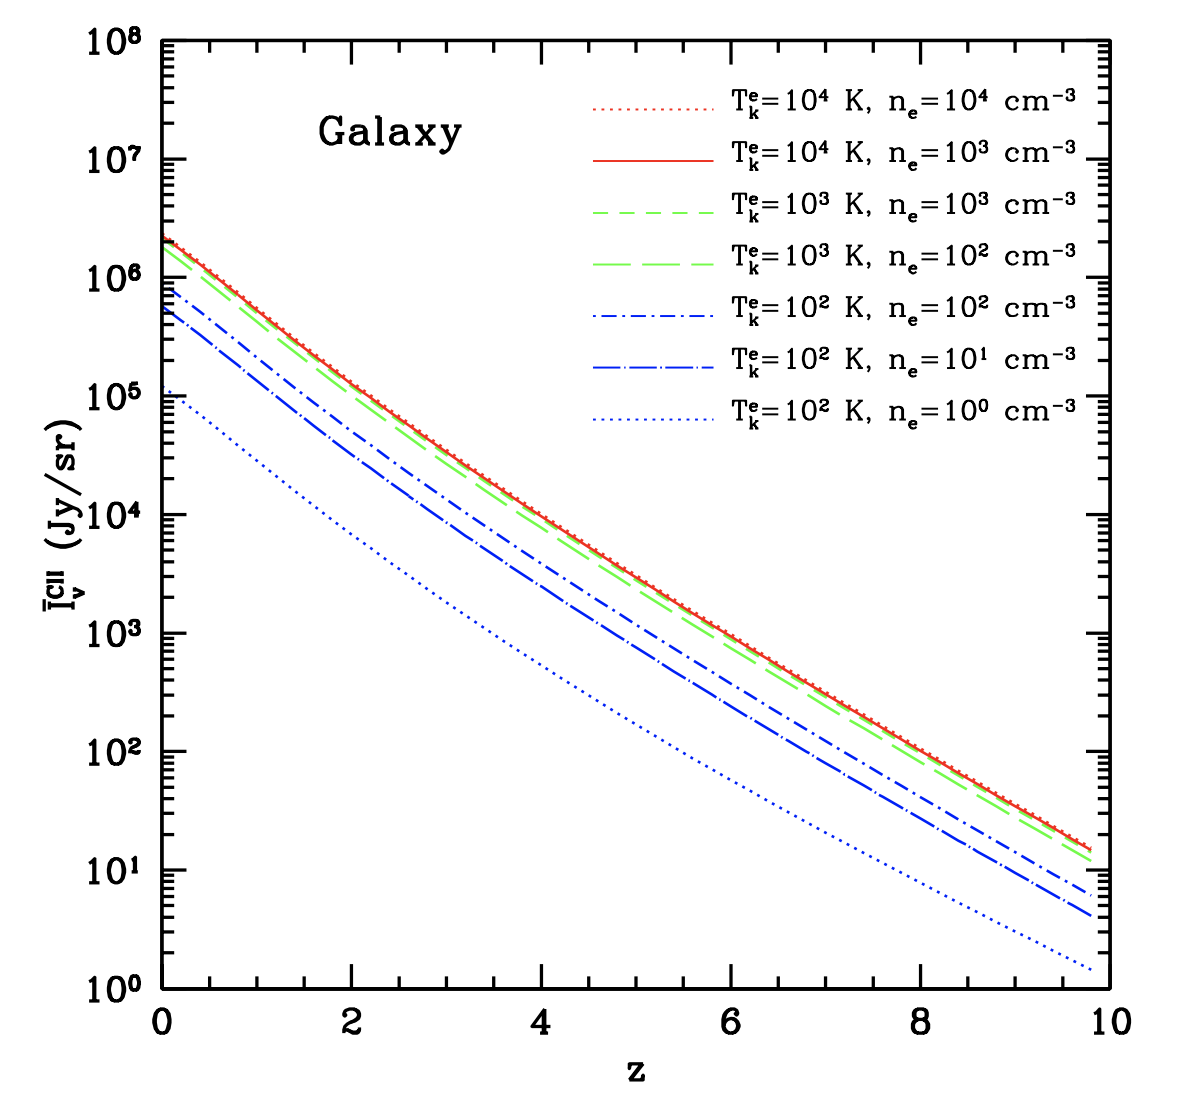
\includegraphics[width=0.4\textwidth]{gong1.png} }}%
    \qquad
    \subfloat{{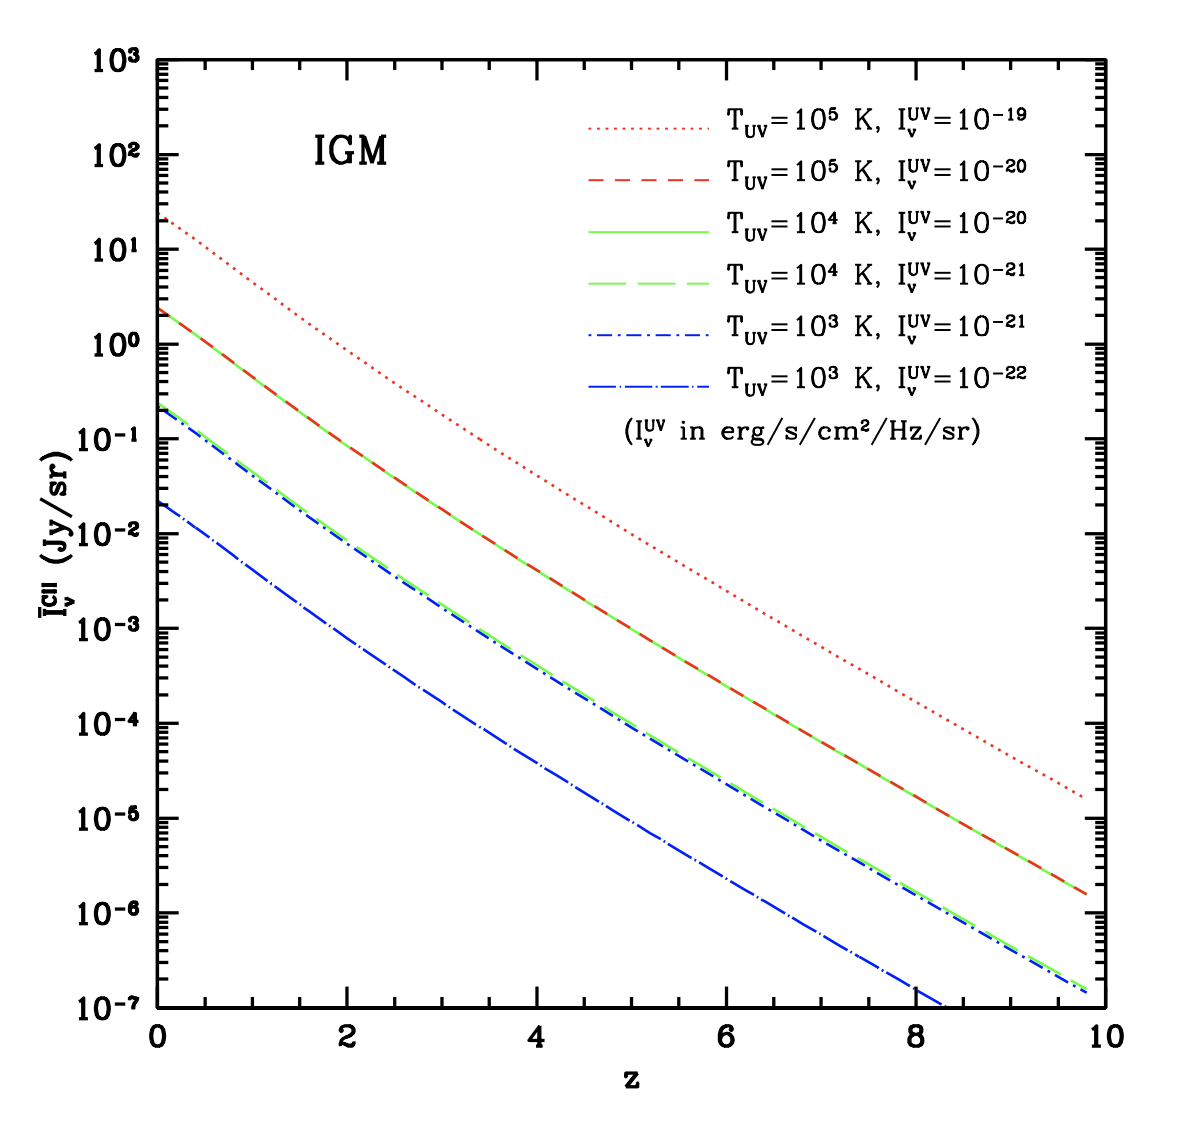
\includegraphics[width=0.4\textwidth]{gong2.png} }}%
    \singlespace
    \caption[Calculated line intensities for CII in the ISM and IGM. -(\cite{Gong2012})]{Left: The expected line intensity of CII for values consistent with the Milky Way ISM at varying redshift, electron temperature, and gas density. Right: Same as left but with IGM parameters substituted. It is clear that the CII intensity in both cases saturates at some critical value, and that the IGM does not contribute as significantly to the overall CII emission [\cite{Gong2012}].}%
    \label{fig:gong1}%
    \vspace{-0.8cm}
\end{figure}

These plots reveal that the CII intensity is predicted to have an increasing trend with redshift, and that the signal is high enough to be detected above shot noise and cosmic variance\footnote{In this case, cosmic variance refers to the fact that observing one region of space will not reveal the actual statistical properties for other regions, due to the random distribution of large scale structure.} in the total CII power spectrum. The power spectrum also reveals the distribution of galaxies during re-ionization, and can reveal how matter was clumped to produce the strength of emission observed. 

It should be noted that the above analytical model agrees well with simulations of galaxies that tune their parameters to match those of observations. However, one physical affect that has not yet been taken into account is line contamination from foreground sources. The rotational and vibrational transitions of CO molecules at low redshift have a similar intensity to those of CII at high redshift, and can contaminate the assumed detection of CII. CO lines  can add as much as 2-30\% change in the apparent CII brightness, leading to incorrect assumptions about the physics of the ISM [\cite{Gong2012}]. Contamination by CI and NII are also present, but not to the same degree as CO. The expected detection of CO and CII by TIME is plotted in Figure ~\ref{fig:coc2power}[\cite{Crites2014}].

\begin{figure}[H]
\centering
\captionsetup{width=0.6\textwidth}
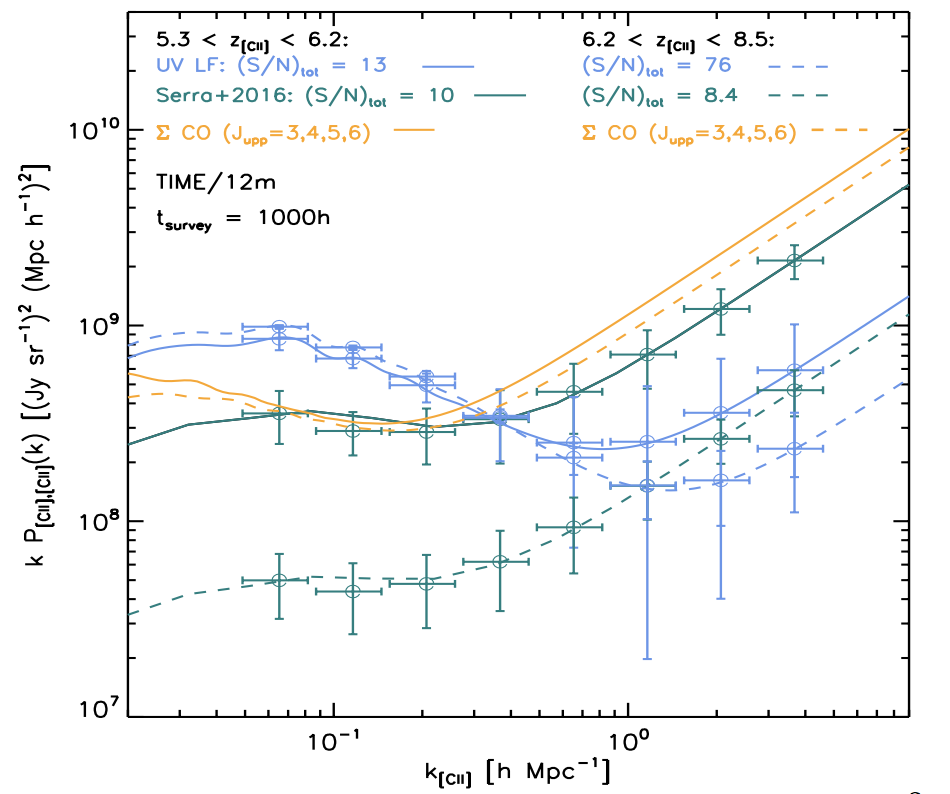
\includegraphics[width=0.6\textwidth]{bock1.png}
\caption[The expected power spectrum for CII and CO using TIME. -()]{The expected power spectrum for CII and CO using TIME for 1000 hours of integration time on the ALMA 12 meter prototype antenna at Kitt Peak. Values for CII were generated from a luminosity function developed by Serra et al 2016. Models of the UV luminosity function were made by observations with HST. Measurements of CO were cast from low redshift into the CII regime\footnote{Reproduced with permission by the TIME Collaboration}.}
\vspace{-0.8cm}
\label{fig:coc2power}
\end{figure}

\subsubsection{Carbon Monoxide: A Star Formation Proxy}

While the word ``contaminant'' has been used to describe CO, it also may present a unique opportunity to probe a different property of the ISM, the molecular gas from which stars are formed. The CO transitions that TIME is sensitive to are present from $0.5 < z < 2$, the peak of star formation [\cite{Madau2014}] down to the more local universe.  With CO, it can be established whether the significant decline in star formation rates is due to the depletion of the cool gas reservoirs in galaxies, or from some other source. The majority of high redshift star formation data is from UV, optical and IR observations, which rely on having a minimum brightness consistent with only the most luminous of the galaxies, and most likely are not representative of the true galactic population. These sources of emission are also caused by hot ionized gas in the ISM, which is not sensitive to the cool gas reservoirs. As with CII, the method of intensity mapping can detect the faintest population that other detections can't reach, and can reveal the potential of those galaxies to produce future stars. By monitoring the cool gas of the ISM, the complete history of the rise and fall of the Epoch of Peak Star Formation can be traced, and the cosmic CO luminosity density can be mapped (\cite{Kovetz2017}). 

This still depends on understanding the correlation between CO and H2, which has been a consistent uncertainty for many other scientific missions. Currently, the best conversions are done using H2 to CO conversions consistent with Milky Way measurements of gas densities, but these are not necessarily valid for high-redshift galaxies. The most common relationship used is that between the far-IR and CO luminosity which, in turn can also be related back to the total star formation rate density. 
\begin{equation}\label{eq:breysse1}
\frac{L_{FIR}}{L_{sun}} = C_{FIR}(\frac{L'_{CO}}{K km s^{-1} pc^{2}})^{X_{FIR}}
\end{equation}
The constants $C_{FIR}$ and $X_{FIR}$ have been observationally determined, and the values are consistent across multiple redshifts. Higher redshift galaxies typically have a lower metallicity, allowing for easier dissociation of CO from a lack of shielding by dust, but a consistent H2 density. Knowing this conversion factor accurately can therefor still provide reasonable gas estimates of H2.  Far-IR luminosities have been measured with high accuracy, which makes this a feasible calculation (\cite{Carilli2013}).  $L_{FIR}$ can then be used with the Kennicutt relationship for star formation rates, which was derived through an estimation of the Schmidt law index (\cite{Kennicutt1998}), where $C_{SFR}$ is a conversion factor between far-IR luminosities and star formation rate that is observationally determined. 
\begin{equation}\label{eq:breysse2}
\frac{SFR}{M_{sol}/yr} = C_{SFR}\frac{L_{FIR}}{L_{sol}}
\end{equation}

Equations ~\ref{eq:breysse1} and ~\ref{eq:breysse2} were taken from \cite{Breysse2016}, in their effort to determine SFRD from CO emission using intensity mapping.  They present a pessimistic uncertainty of 50\% in the conversion between CO luminosity and star formation, but also admit that if intensity mapping could be compared with other galactic features, this model uncertainty would decrease, with intensity mapping creating a significant improvement to the redshift dependence of CO.  

The predicted CO signal produced by galaxies of varying masses and redshifts is given by \cite{Visbal2010}, who include two terms  $f_{\star}$ and $\epsilon_{duty}$, which correspond to the halo star formation efficiency and 
duty cycle (the fraction of time it takes for the galaxy to emit detectable levels of radiation). 
\begin{equation}
L = 6.6\times10^{6}(\frac{R}{3.8\times10^{6}})(\frac{M}{10^{10}})(\frac{1+z}{7})^{3/2} \frac{f_{\star}}{\epsilon_{duty}} L_{sol}
\end{equation}
These two terms are once again based on observation and modeling, and carry their own intrinsic error. 

\subsubsection{CII-CO Separation}
CO has the potential to make advancing contributions to our understanding of the gas reservoir of high redshift galaxies. 
\begin{wrapfigure}{r}{0.5\textwidth}
\vspace{-0.8cm}
  \begin{center}
    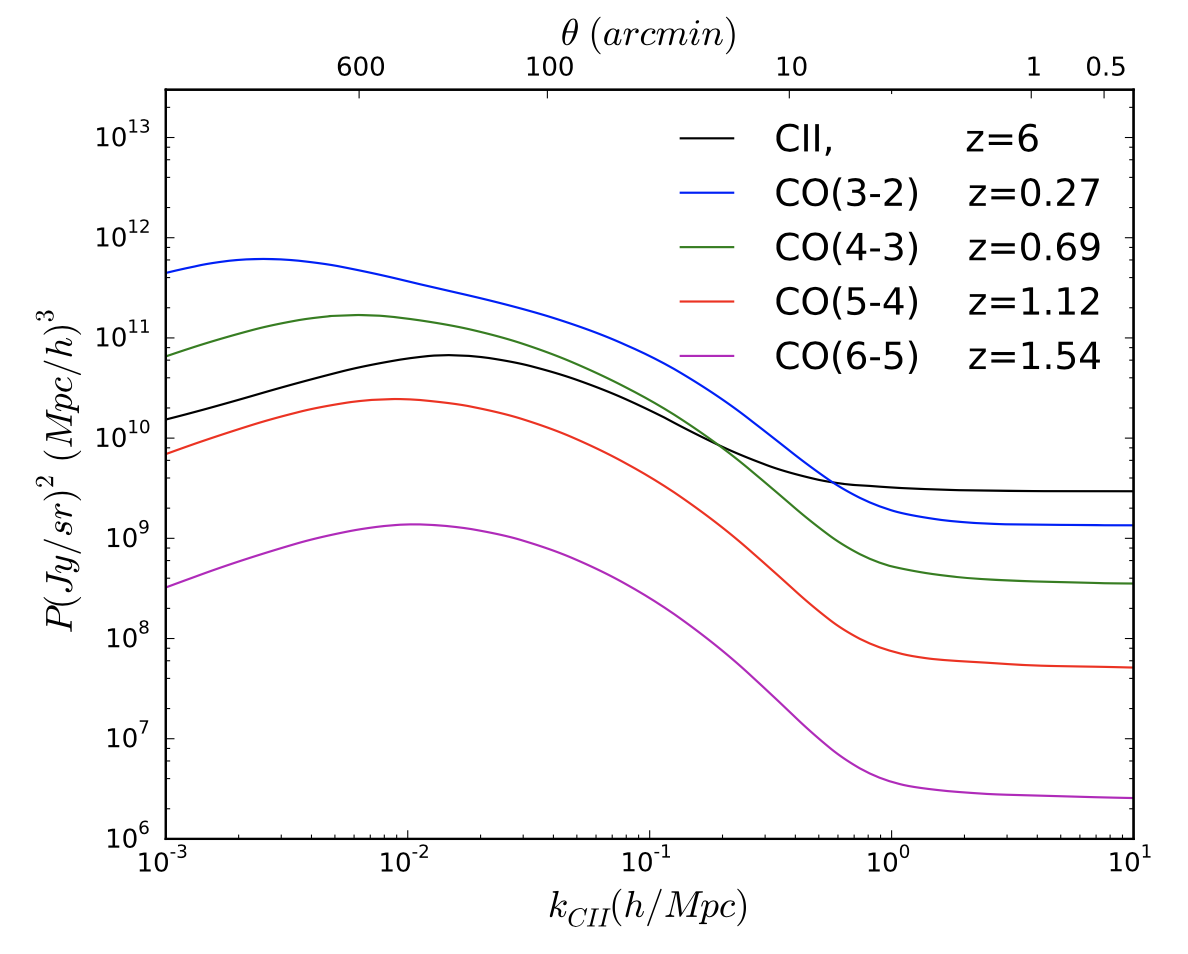
\includegraphics[width=0.48\textwidth]{cheng1.png}
  \end{center}
  \caption[Calculated CO and CII power spectrums, showing the difficulty in separating the two signals. -(\cite{Cheng2016})]{Calculated CO and CII power spectrums for a simulated universe, with the apparent mixing of the signals at various scales for specific CO transitions. Lower redshift CO transitions consistently contaminate the higher redshift CII signal at every scale length (\cite{Cheng2016}).}
\end{wrapfigure}
However, since the CII and CO intensities are confused for high redshift measurements, no insights will happen unless the two signals can be disentangled (see Figure 6). Two distinct methods have been proposed by the TIME group to accomplish this task. This can in part be accomplished through correlations of the estimated CO signal with other metrics such as far-IR. As was discussed above, some empirical relationship exists between the CO and far-IR luminosity, which can be used to separate it from the CII intensity.  

A more complicated, but slightly less model dependent method is based on the geometrical separation of the two signals in power space. Both the signal for CO and CII have power spectrums that are redshift dependent, but each redshift dependence is unique. Consider a CII line intensity measured for a z = 6 galaxy with some unknown CO component, and the power spectrum is created under such an assumption, but the CO line intensity is actually from a z = 2 galaxy. When the transformation of the intensity to power spectrum is made under the z = 6 assumption, the CO dependence on redshift will be incorrectly assigned, and show a pattern which is inconsistent with the ``real'' data. This is analogous to thinking about the intensity of the lines within their own frame. To an observer at z = 6 and z = 2, the CII and CO line intensities respectively, appear isotropically emitting. However, if this CO line is transformed to a z = 6 frame, the signal becomes anisotropic and distorted, relative to the CII intensities.  

%This method relies on the apparent isotropy of the emission within its own frame, and the conversion of this emission into the comoving frame. By creating a redshift projection of the emission onto the comoving frame, the new emission has an anisotropic pattern that is dependent on redshift. However, when two emissions at two separate redshifts are transformed into the same comoving coordinates, they both exhibit different anisotropic patterns. %

An example of this technique was given in \cite{Cheng2016}, who created a realistic universe based on $\Lambda CDM$ cosmology and generated the CO and CII power spectra. Their simulated spectra is shown in Figure 6, with the mixing of the CII and CO spectrum clearly evident. The next two graphs show the change in the anisotropic patterns at z = 6. It is easy to see that the two anisotropies are projected differently onto z=6 depending on their actual redshift.

\begin{figure}[h!]
    \centering
    \subfloat{{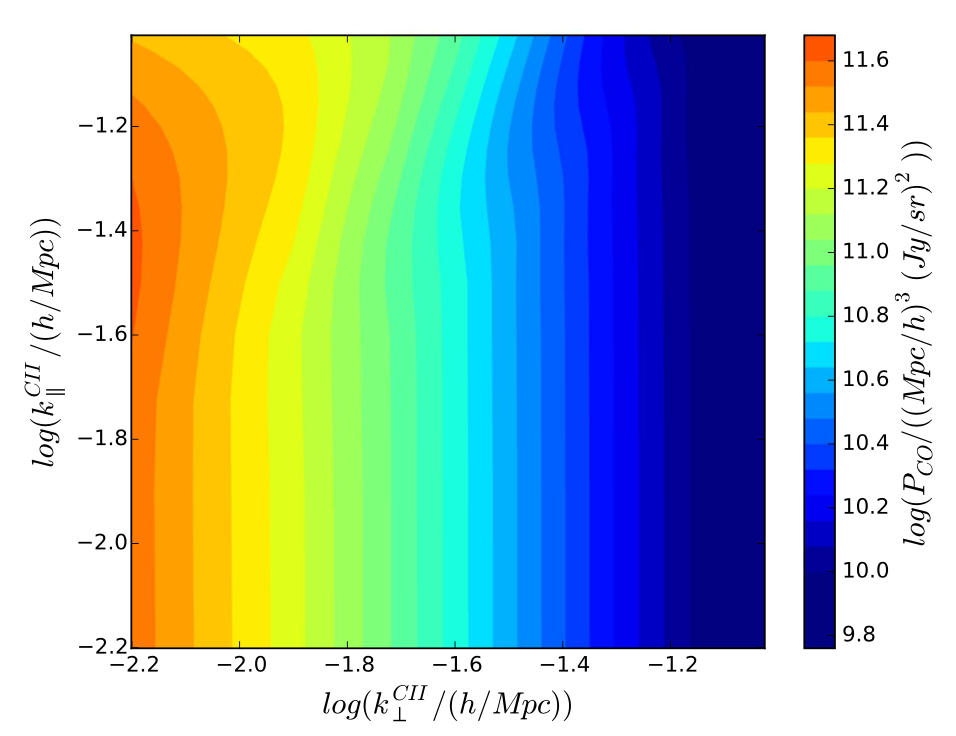
\includegraphics[width=0.45\textwidth]{cheng2.png} }}%
    \qquad
    \subfloat{{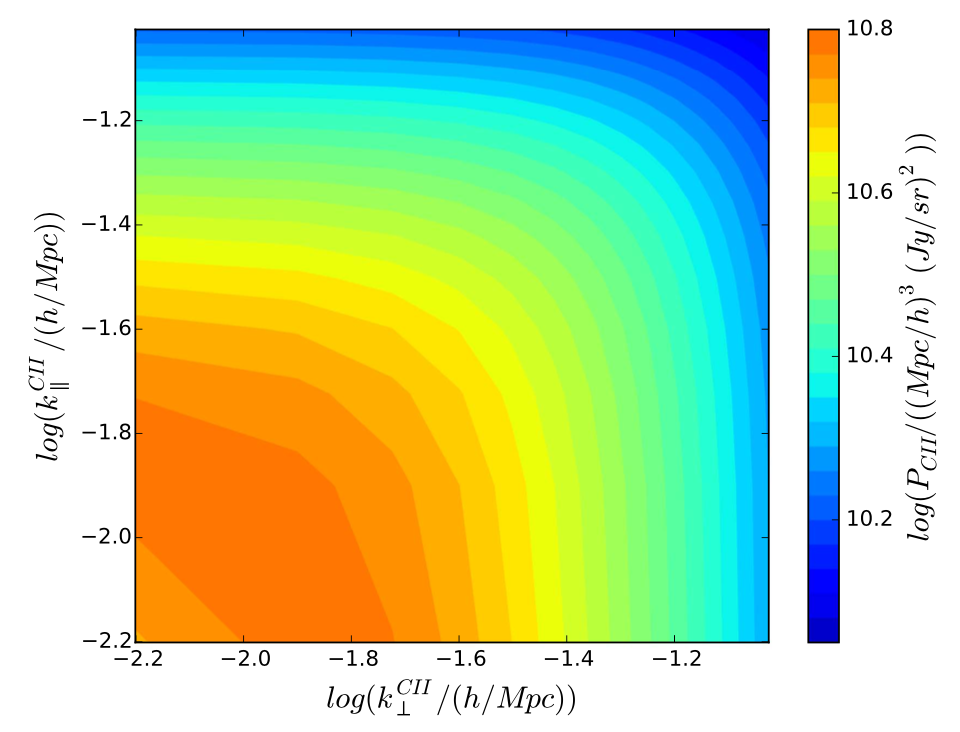
\includegraphics[width=0.45\textwidth]{cheng3.png} }}%
    \singlespace
    \caption[Deblending of the CII and CO power spectrums. -(\cite{Cheng2016})]{Deblending of the CII and CO powerspectrum. Both figures represent CII power spectra data from z=6. However, the right figure has been incorrectly processed using a z=2 model, changing the uniform spectrum to an anisotropic one (\cite{Cheng2016}).}%
    \label{fig:cheng1}%
\end{figure}

\subsubsection{CII-CO-21 cm Cross Correlations}
The TIME instrument is not designed to detect 21cm emission, however, it has been noted by some authors (\cite{Zaroubi2012},\cite{Gong2012}) that it is a useful comparator with CII and CO for determining evolutionary properties within the ISM and IGM. 
%However, in order for it to be a useful correlator, it must also have some intrinsic scientific value, and have a relative spin temperature above that of the CMB. 
21cm traces neutral hydrogen reservoirs, with a spin temperature that is highly sensitive to the physical processes at work including gas dynamics and feedback. Understanding the evolution of this tracer can lead to a more thorough understanding of these processes through the EOR. 

The 21cm line is a forbidden transition between the hydrogen triplet and singlet state, where the orientation of the spin axis is ``flipped'' between the proton and electron. While the spontaneous emission of this line has a decay on order $10^{7}$ years, the high abundance of neutral hydrogen makes this transition easily detectable. The measured intensity is sensitive to several different processes, including the absorption and stimulated emission of CMB photons, collisional excitations, and Lyman $\alpha$ pumping. These processes are incorporated into the effective spin temperature of the emitted photon, which must be of a different temperature than that of the CMB to be detected. Depending on the type of object creating the emission, this spin temperature will show fluctuations even when other parameters are held constant (such as redshift and peculiar velocity). For example, excitation from UV pumping will transfer a specific amount of energy to the surrounding atomic hydrogen depending on the energy of the photons and the optical depth of the neutral medium. Excitation due to x-ray sources however have energies too high to create 21 cm spin flips, but can cause collisional excitation due to scattering electrons. The strength of the x-ray emission will determine the energy of the collision, and how many scattering events will happen. It could also produce collision ionization and heating. By carefully mapping the intensities of 21 cm emission, the types of EOR objects ionizing the IGM can be determined (\cite{Zaroubi2012}).

\begin{figure}[H]
	\centering
	\subfloat{{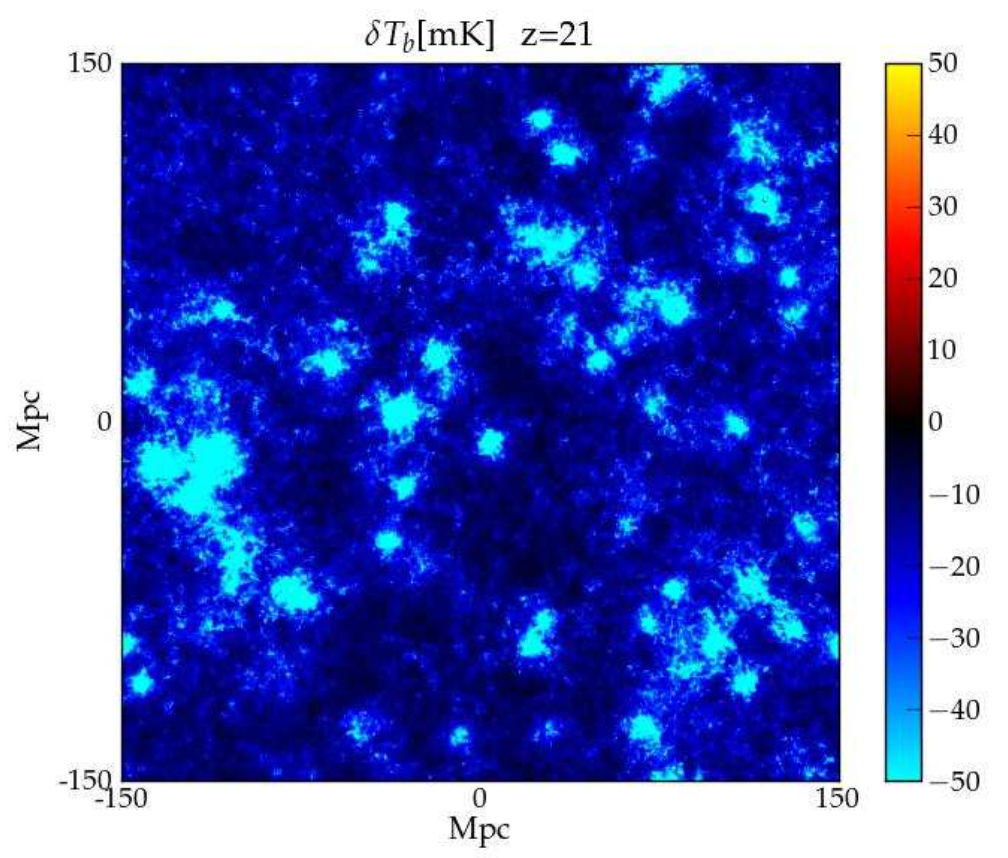
\includegraphics[width=0.45\textwidth]{santos1.png} }}%
	\qquad
	\subfloat{{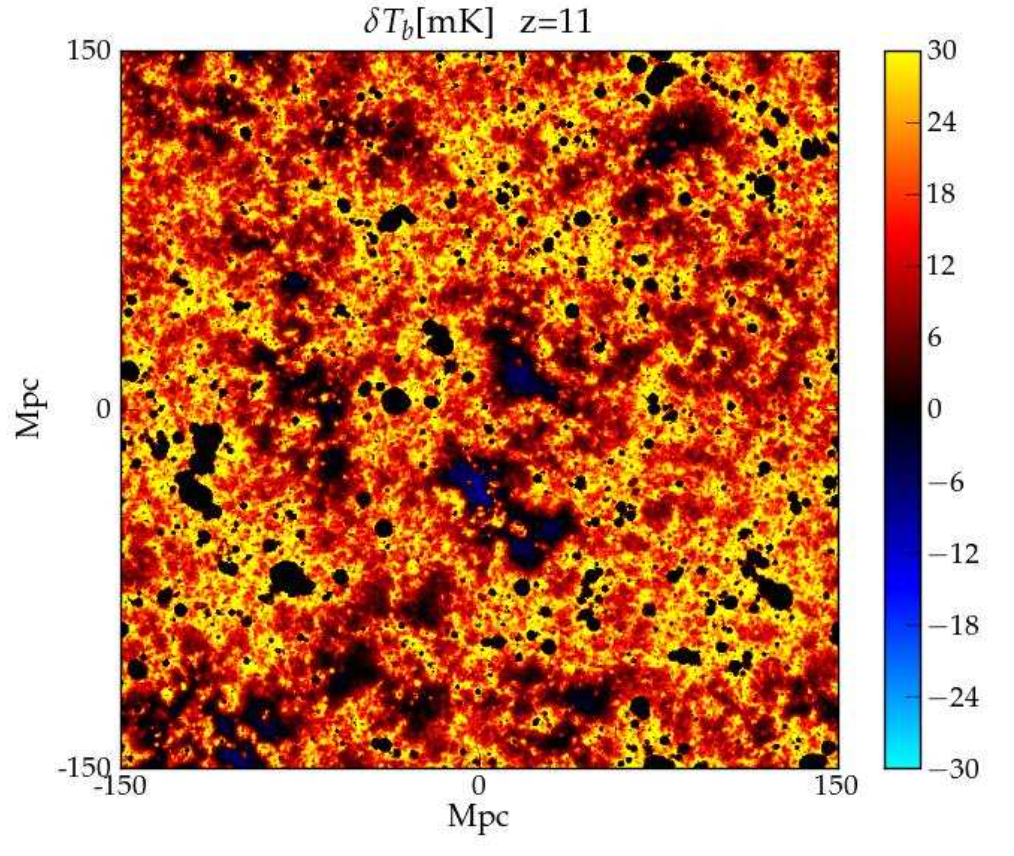
\includegraphics[width=0.45\textwidth]{santos2.png} }}%
	\singlespace
	\caption[21 cm brightness maps for different redshifts. -(\cite{Santos2010})]{Results of simulations for 21 cm brightness variations with space and redshift. An evolution of ionization pockets can clearly be seen, with both an increase in the size and number of ionizing source with decrease in redshift (\cite{Santos2010}).}%
	\label{fig:santos1}%
\end{figure}

As was mentioned above, a comparison between CII and 21 cm, where both are tracing the ionization history of the ISM, can be very fruitful. CII is essentially a proxy for neutral hydrogen abundances, while 21 cm probes this population directly, making it useful for corroborating CII gas mass estimates. In addition, both are tracing the same density field, meaning their power spectrums will allow an angular scale determination for ionization bubble size with redshift. \cite{Santos2010} created simulated power spectra for both galaxy halo mass and 21 cm emission to predict the evolution of the EOR with redshift. The evolution of the ionization bubble size can easily be seen in Figure ~\ref{fig:santos1} from snapshots taken from redshifts of z = 21 and z = 11 in the simulation. It can be seen that the ionization of the ISM increases significantly, and the ionization of the IGM starts to become more complete at z = 11. 

\cite{Gong2012} coupled these 21 cm brightnesses with the expected CII intensity to create a cross-correlation coefficient calculated by \(r_{CII,HI}(k) = P_{CII,HI}(k)/\sqrt{P_{CII}(k)P_{HI}(k)}\). The mean ionization bubble size corresponds to the region where the coefficient reaches zero (from negative values) in Figure ~\ref{fig:gong1}. For z = 6, this corresponds to a larger scale than that for either z = 7 or z = 8, consistent with the higher redshift models from the \cite{Santos2010} simulations. 
\begin{wrapfigure}{r}{0.5\textwidth}
\vspace{-0.8cm}
  \begin{center}
    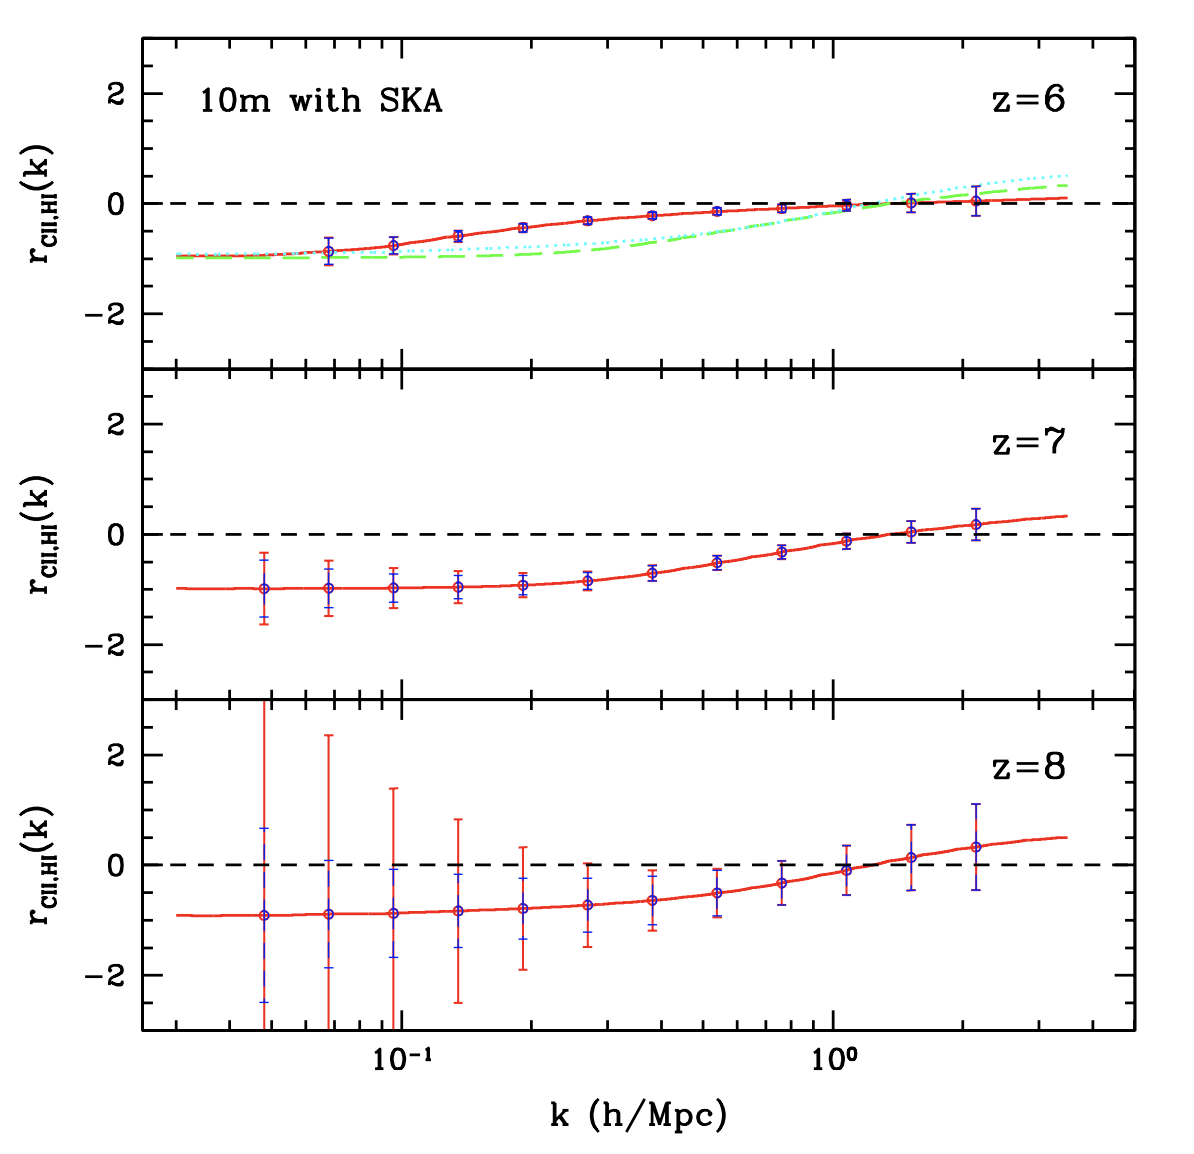
\includegraphics[width=0.48\textwidth]{gong4.png}
  \end{center}
  \caption[Cross correlation coefficient for CII and 21 cm showing ionization bubble size with redshift. -(\cite{Gong2012})]{Cross correlation coefficient for CII and 21 cm for changing scale sizes. There is a clear change in the scale of negative to positive correlation for changing redshift, indicating the average scale size for ionization bubbles (\cite{Gong2012}).}
  \label{fig:gong1}
  \vspace{-0.8cm}
\end{wrapfigure}
This particular model was created using an assumed millimeter spectroscopic survey and the 10m Square Kilometer Array. It should be noted that this same comparison can also be done with CO, but the correlation is slightly different. For large scales, CO is anti-correlated with 21 cm, since the CO implies an increase in the number density of galaxies and ionization, but a decrease in the neutral 21 cm intensity. For small scales, these two metrics are fairly uncorrelated, since CO no longer necessarily traces with galaxy counts and the neutral medium is also too small to contain a galaxy. This CO-21cm anti-correlation traces the size of large scale structure and neutral hydrogen reservoirs, allowing a determination of the ionization bubble sizes as well. 

%================================================================================================================
\subsection{Objective 2: The SZE and the Evolution of Large Scale Structure}

Study of kSZE has impacts for understanding both the internal gas physics and dynamics of clusters, but also for cosmology as well. In order to understand why, it is necessary to review the process by which this phenomenon is created. There are in fact two distinct flavors of the SZ phenomenon which are split into a thermal and a kinetic effect. The thermal effect is due to a thermally induced motion of intra-cluster medium (ICM) electrons, whereas the kinetic effect probes the bulk motion of cluster gas. Both, are detected as temperature fluctuations in the anisotropic signal of the CMB, and measured as a change in the intensity of the CMB signal (\cite{Sunyaev1970}).  The process by which this occurs is Inverse Compton Scattering (ICS), whereby the photons of the CMB become up-scattered by the highly energetic ICM electrons, and re-emitted at more energetic wavelengths. 

For the tSZE, the energy of the CMB photon is increased by a factor of \(\frac{k_{B}T_{e}}{m_{e}c^{2}}\) which in turn causes a 1mK level distortion in the CMB spectrum. This thermal effect also has the interesting property of affecting the CMB differently at different frequencies. For frequencies less than 218 GHz, the intensity of the CMB is decreased, while frequencies greater than 218 GHz the reverse is true (\cite{Carlstrom2002}). 

The kSZE is due to the relative motion of the cluster gas with respect to the CMB, which creates a spectral distortion in the CMB due to the Doppler effect, induced by the cluster bulk velocity.  This distortion changes depending on whether or not the ICM electrons have relativistic energies, however, the underlying Planck Spectrum is preserved. The change in the Rayleigh Jean's temperatures is higher for positive velocities, and lower for negative velocities. For non-relativistic energies, in the rest frame of the gas, the CMB appears anisotropic, where ICS acts to create an isotropic radiation field. In the rest frame of the observer, the radiation field appears anisotropic, with the CMB photon energies increased by a factor of \(\tau_{e} v_{pec} / c\) , where \(\tau_{e}\) is the optical depth of the gas, \(v_{pec}\) is the peculiar velocity and \(c\) is the speed of light. (\cite{Birkinshaw1999}) This relationship provides a very real diagnostic tool of the internal motions of the cluster gas and significant clues about the properties of the cluster itself.

\begin{figure}[!ht]%
    \centering
    \subfloat{{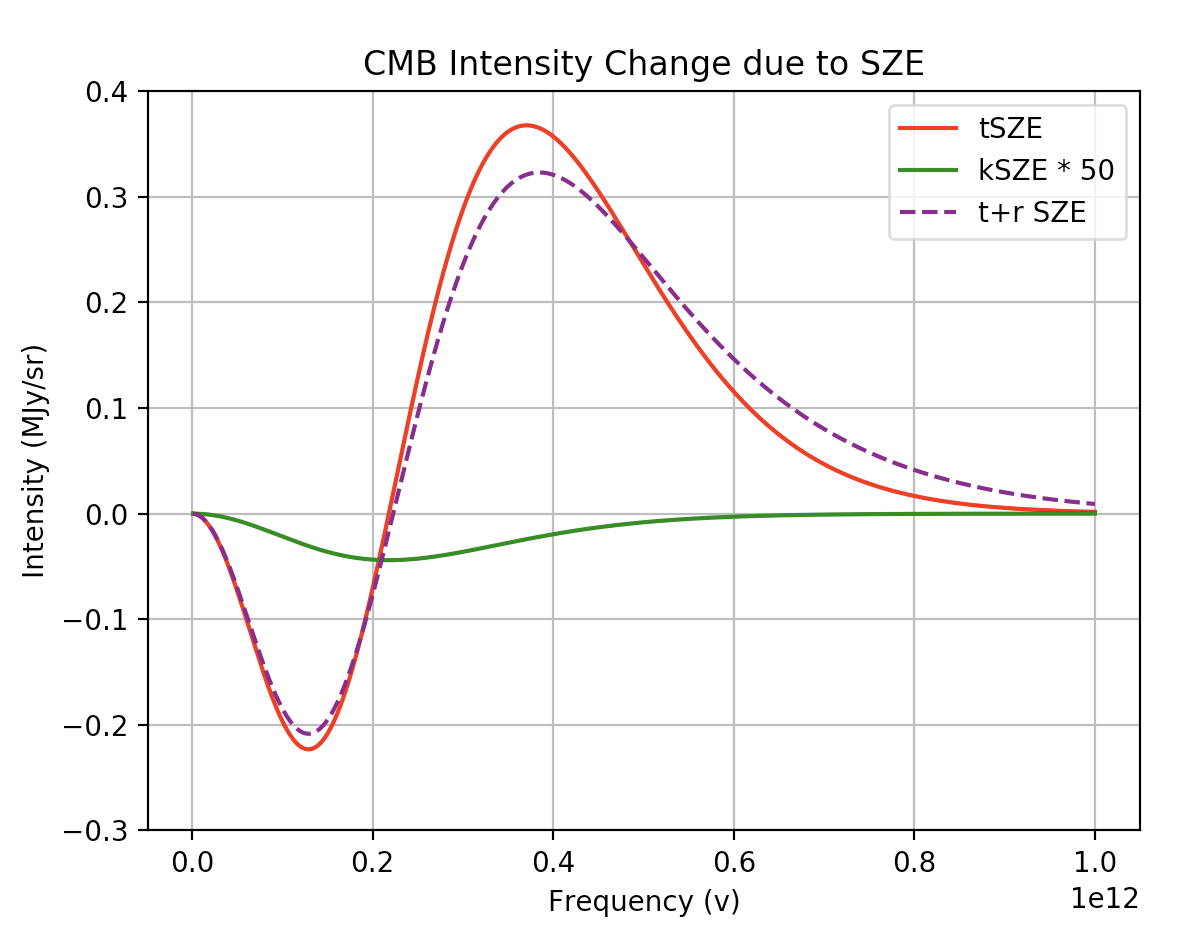
\includegraphics[width=0.45\textwidth]{tkrsze.png} }}%
    \qquad
    \subfloat{{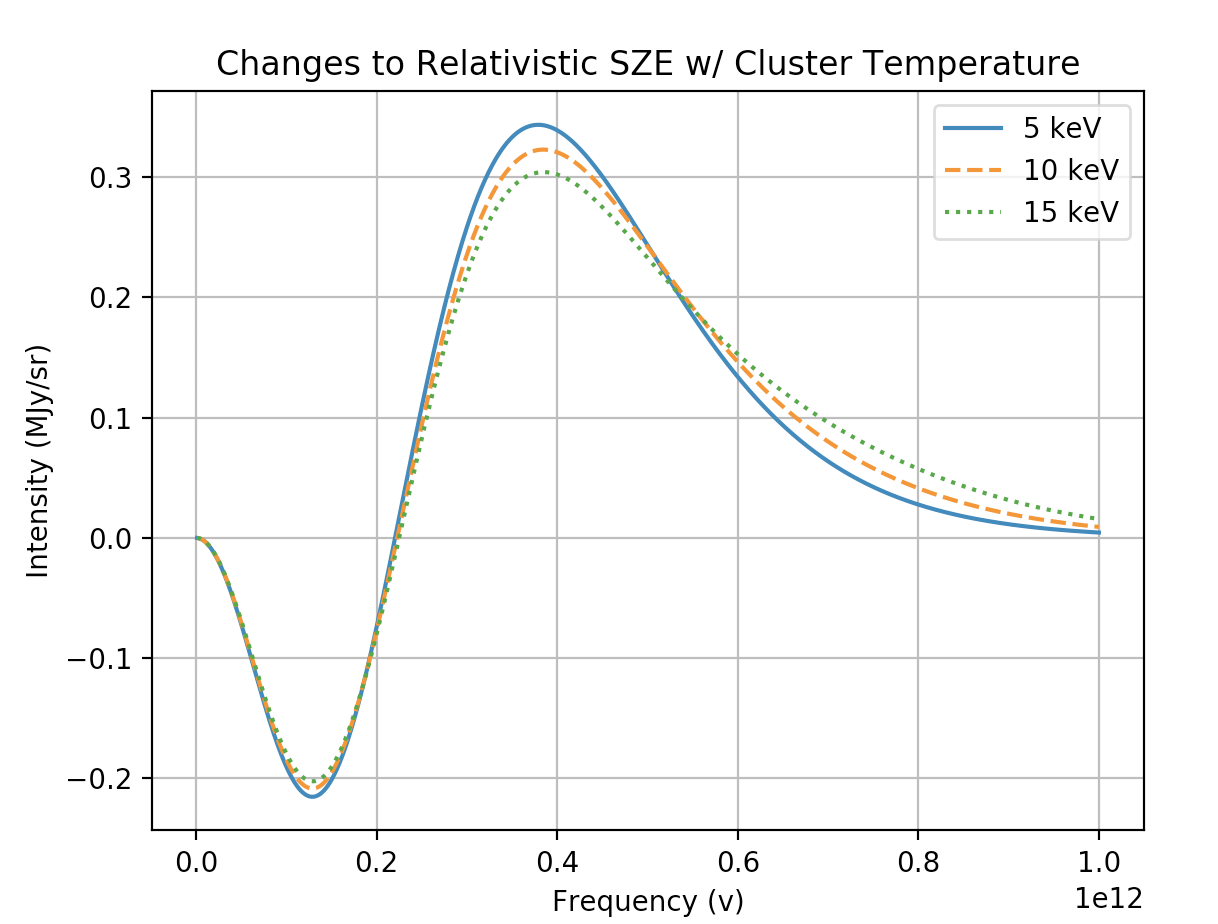
\includegraphics[width=0.45\textwidth]{rsze.png} }}%
    \singlespace
    \caption[Intensities of the kSZE, tSZE, and rSZE for simulated galaxy cluster.]{Left: Relative intensities for the SZE for thermal, kinetic, and relativistic electrons. The kSZE presents as a doppler shift in the CMB intensity and changes from positive to negative depending on the proper motion of the cluster gas. This kSZE was calculated for a clusters with peculiar velocity of -1000 km/s. The thermal effect shows a null at roughly 218 GHz but can shift depending on the properties of the cluster. The relativistic effect is for a cluster with electron temperature of 10 keV. Right: The strength of the relativistic effect at various cluster gas temperatures. The increase in the Rayleigh Jeans tail at higher temperatures makes the detection of the kSZE more attainable.}%
    \label{fig:tksze}%
\end{figure}

Although TIME science will explore primarily the kSZE signal, it is still necessary to measure the tSZE. The reason why is easily seen from Figure 1, taken from \cite{Carlstrom2002}, which shows the relative strengths of both signals in terms of the CMB brightness and the Rayleigh-Jeans brightness temperature. In both cases, the kSZE signal is orders of magnitude fainter than the tSZE, except for one special circumstance. There is in fact a null of the tSZE at 218 GHz, but for which the kSZE effect is still non-zero. This property will become fundamentally necessary for disentangling the kSZE from the tSZE. Not only is the signal much fainter, putting strict lower mass limits on the mass of the cluster observed, but the signal is further confused by CMB anisotropies that, when extracted from the full SZE signal, could remove some of the kSZE along with it. This is due to the fact that the kSZE is the first moment of the CMB, and even with careful modeling, can be difficult to remove entirely. In the case of extremely high mass, rich galaxy clusters, there is a much higher abundance of relativistic electrons, and a much better chance of retrieving a pure kSZE signal, independent of the CMB and the tSZE. For a massive cluster with \(k_{B}T_{e} = 10 keV\), modeling suggests that most electrons are well into the relativistic range. Papers of some of the earliest measured clusters found gas temperatures around \(k_{B}T_{e} = 15 keV\) (\cite{Mushotzky1997},\cite{Allen1998}), with high significance SZE detections.

Perhaps the most important property of the SZE is that it produces a redshift independent measurement. This is due to the fact that the SZE is created by photons from the same 2D surface (the CMB) scattering off of electrons in clusters. Under the assumption that photons at the largest scales have had very little interaction with other particles until reaching a cluster, the source for the photons are all from the same redshift. This is more clearly seen from the equation describing the relativistic maxwellian distribution of electrons, like the ones that would be found in the ICM of massive clusters. Equation ~\ref{eq:boltzman} below is taken from \cite{Birkinshaw1999} and shows the intensity change to the CMB from relativistic ICM electrons. \(P_{1}(s)\) is a scattering function for SZE,  and \(\tau_{e}\) is the optical depth for the electrons. Interestingly, nowhere contained within Equation 3 are any signs of redshift dependence.

\begin{equation}\label{eq:boltzman}
\Delta I(\nu) = \frac{2h}{c^{2}}\tau_{e} \int_{-\infty}^{\infty} P_{1}(s) ds (\frac{\nu_{0}^{3}}{e^{h\nu_{0}/k_{B}T_{rad}}-1}  - \frac{\nu^{3}}{e^{h\nu/k_{B}T_{rad}}-1})
\end{equation}

It should be noted that while this equation is redshift independent, it does depend somewhat on cluster properties, such as assumptions that the cluster gas is optically thin, and that the temperature of the gas is in hydrodynamic equilibrium at a constant temperature. Any changes to these parameters would change the resulting spectral distortion of the CMB. The change of these cluster properties could be well modeled after the first surveys of the SZE, as it is suspected that higher redshift clusters are more compact, meaning that the gas temperature function should show a positive trend with increasing redshift. Since this equation is for a relativistic treatment of electrons, we also need a dense, hot massive cluster for it to apply, which sets a somewhat stringent mass limit for detection of the relativistic effect (\cite{Carlstrom2002}).

Fortunately, it is also possible to create an analytical function for non-relativistic electrons through the application of the Kompaneets equation (\cite{Birkinshaw1999}).

\begin{equation}
I(\nu) = \int_{-\infty}^{\infty} P_{K}(s) I_{0}(\nu_{0}) ds
\end{equation}
\begin{equation}
P_{K}(s) = \frac{1}{\sqrt[2]{4 \pi y}} exp(-\frac{(s + 3y)^{2}}{4y}
\end{equation}

\(I_{0}\) describes the blackbody spectrum of the CMB, \(P_{K}\) is the scattering function, and y is the comptonization parameter given by \(y = \int   n_{e}   \sigma_{T}   dl   \frac{k_{B}T_{e}}{m_{e}c^{2}}\) .

While this is simply theory, some of the first interferometric observations of clusters at multiple redshifts confirmed that the SZE had the same ratio to the CMB brightness across a wide range of redshifts. Figure 2, taken from \cite{Carlstrom2002}, shows this redshift-independent feature.

\newpage
\begin{figure}[H]
\centering
\captionsetup{width=0.85\textwidth}
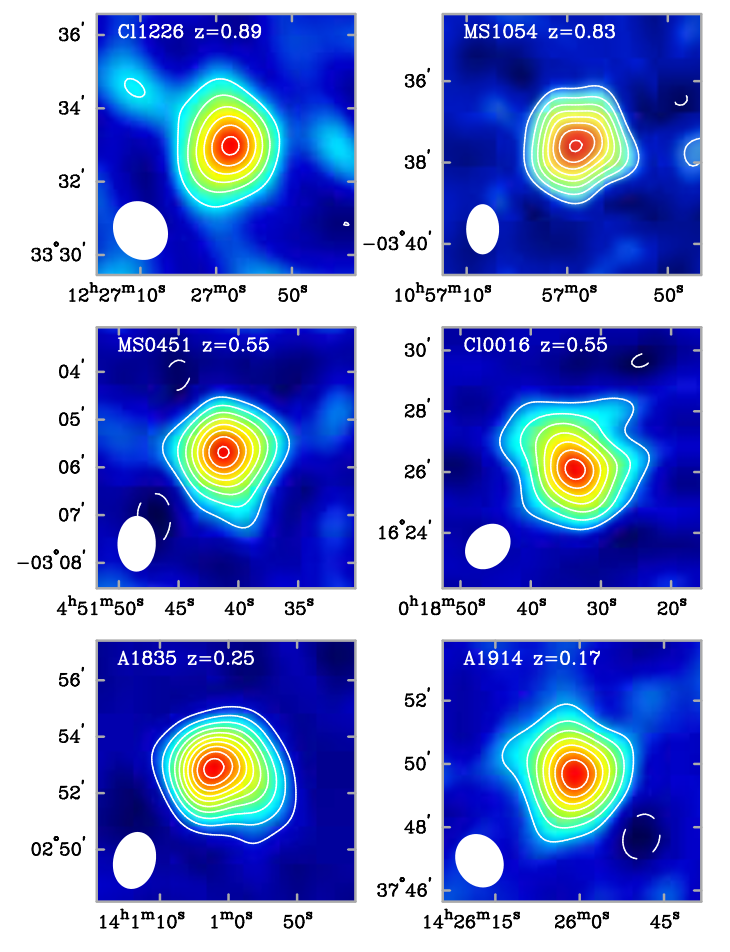
\includegraphics[width=0.85\textwidth]{carlstrom1.png}
\caption[An example of the redshift independence of SZE measurements for six different clusters. -(\cite{Carlstrom2002})]{Deconvolved interferometric SZE images for galaxy clusters between z = 0.17 and z = 0.89. Isophotal contours at multiples of \(2\sigma\) are also shown in white solid lines. In the bottom left corner, the FWHM of the beam ellipse is also shown. The signal appears to suffer from no cosmological dimming as a function of redshift, as the relative intensity across each cluster is roughly the same (\cite{Carlstrom2002}).}
\end{figure}
%%

\subsubsection{kSZE Implications for Cosmology}

After the formation of the universe in the Big Bang, the temperature was so high that only subatomic particles could survive. Radiation was the dominant energy density, where particles were still heavily coupled to the cosmic plasma. Afterwards, a brief inflationary phase magnified any quantum fluctuations in the surrounding medium and rapidly reduced the temperature to the point where atomic nuclei could form (recombination) and photons decouple (decoupling). Those photons have been propagating ever since, with little interaction, and still retain a perfect Blackbody spectrum, known as the Cosmic Microwave Background (CMB). 

This is a theoretical timeline for the early history of the universe, but with some uncertain epochs, including when dark matter particle production began. Current models [CITE SOURCE HERE] assume that it is before decoupling, where there was enough time for it to couple to baryonic matter and initiate gravitational collapse. These gravitational instabilities are observable in the power spectrum of the CMB, with the first mode sensitive to the present day distribution of large scale structure. What is still unknown is the evolutionary process from those first gravitational instabilities to the largest gravity potential wells created by galaxy clusters. 

One method to understand the role of dark matter in this evolution is through the Boltzmann Equations for cold dark matter particles. A version of a first order solution, taken from \cite{Dodelson2003}, is shown in Equation 1. Here, the overdots are derivatives with conformal time, where \(\delta\) is the dark matter overdensity, k is the magnitude of the wavevector (which in Fourier space is analogous to the three-space coordinate x), and v is the velocity of the dark matter particles. The quantities are related to the gravitational potential that the particles exert on the surrounding space-time metric.

\begin{equation}
\dot{\delta} + ikv = -3\dot{\Phi}
\end{equation}

Additionally, the overdensity of dark matter can also be related to the observed anisotropy  through Equation 2, also taken from \cite{Dodelson2003}. The variable \(\Theta_{0}\) corresponds to the monopole of the perturbation of the matter density field, at a given point from its average over all space, and the other two variables are consistent with those above. From this, it is easily seen that an overdense region produces a reduction in the observed CMB anisotropy. This is due to the the photon losing energy as it attempts to move outside of its potential well. Regions with more dark matter, and more baryonic matter, have larger potential wells, and will have a more negative anisotropy compared to underdense regions. 

\begin{equation}
(\Theta_{0} + \Phi)(k,\eta_{\star}) = -\frac{1}{6} \delta(\eta_{\star})
\end{equation}

It should be noted that this solution is valid only for large-scale modes, which is appropriate for galaxy clusters. The methodology for extracting the physical properties of galaxies is much more convoluted for non-linear regimes, as many other contaminating elements, namely dipole and quadropole fields (an example of a quadropole field being gravitational waves) create a difficult solution to the Boltzmann equations. The relationship between the anisotropies and the underlying physics of the system are much harder to correlate in that instance. 

Work has also been done to show the relationship between the emitted photons and the physics of the cluster, based on the measured CMB brightness. The equation below taken from \cite{Dodelson1995} shows the change in the CMB brightness depending on the number density of the electrons in the cluster and the gas peculiar velocity. This first order solution to the Boltzmann Equation is derived assuming a flat, matter dominated universe, and only includes terms which are caused by the relative motion of the gas. Higher order effects have been ignored. The $\Delta$ are the relative change in the CMB brightness, $n_{e}$ is the electron number density, $\sigma_{T}$ is the Thompson scattering cross section, a is the cosmic scale factor, and the $4 \mu \tilde v$ is the doppler shift term due to the motion of the electrons. The derivative is over conformal time, with the tildes denoting Fourier space. 

\begin{equation}
\dot{\tilde \Delta} + ik\mu \tilde\Delta = n_{e} \sigma_{T} a (4 \mu \tilde v - \tilde \Delta)
\end{equation}

While these equations make it apparent that studying the CMB anisotropies would lead to insights about the dark matter densities in galaxy clusters, it also implies that anything that modifies the local gravitational potential would create deviations from the expected temperature fluctuations. The kinematic effects on the CMB photons from the peculiar velocities of the electrons shown in Equation 3 show a very similar dependence to that of gravitational potentials of the clusters themselves. This leads to the conclusion that the properties of dark matter on large scales can be derived from the kSZE. 

Cluster velocities measured with respect to the positions of other large scale structures are often referred to as bulk velocities, and have predicted values based on standard cosmology.  Traditionally, bulk flows are determined using peculiar velocities obtained optically, given a fairly close cluster and high resolution telescope. The distance is estimated with photometric, or if available, spectroscopic redshifts, which are more subject to errors with an increase in distance. As explained above, SZE measurements do not suffer from such redshift effects.

Simulations like Illustrus [CITE SOURCE HERE] show this bulk flow particularly well for clusters that are within a cosmic filament, or region of overdensity, where individual clusters are drawn towards the large potential well created by the abundance of dark matter. An example from our local universe would be the ``Great Attractor'', a region of galaxy overdensity with respect to redshift. For a typical spherical region of radius R, the bulk velocity should decrease linearly with comoving distance under standard cosmological parameters, with values around \(v_{rms}(r > 50-100  h^{-1} Mpc) = 250 km/s\) (\cite{Mak2011}). Since this velocity is believed to be caused by both baryonic and dark matter, it can be related back to the surrounding density fluctuations via ~\ref{eq:bulkvelocity}. 
\begin{equation}\label{eq:bulkvelocity}
 <v^{2}_{\parallel}(r,z)> = \frac{H_{0}^{2}E(a)^{2}a^{2}}{6\pi^{2}} \int_{0}^{\infty} (\frac{d ln D}{d ln a})^{2} P_{m}(k,z)|\tilde{W}_{r}(k)|^{2} dk
 \end{equation}
\(\tilde{W}_{r}(k)\) is the 3D Fourier transform of a real space top-hat filter over a comoving sphere of radius r, \(P_{m}(k,z)\) is the matter power spectrum, and E(a) is the energy density change with scale factor. This allows a direct comparison of cluster velocities to the predicted matter power spectrum, as observed using the CMB.

%=======================================================================================
%(Bhattacharya \& Kosowsky 2008):

%we describe the dark energy in terms of three phenomenological parameters: its current energy density ΩΛ, and two parameters w0 and wa describing the redshift evolution of its equation of state w(a) = w0 +(1−a)wa. Assuming a spatially flat universe, the set of cosmological parameters p on which the velocity field depends are the normalization of the matter power spectrum σ8 (or equivalently the normalization constant B in Eq. (5)), the power law index of the primordial power spectrum nS, and the Hubble parameter h, plus the dark energy parameters.

%Even for velocity errors as large as 1000 km/s for individual clusters, a velocity catalog for several thousand clusters can improve dark energy constraints from the corresponding cluster number counts by a factor of two

%For upcoming Sunyaev-Zeldovich galaxy cluster surveys, even velocity measurements with errors as large as 1000 km/s will substantially improve the cosmological constraints compared to using the cluster number density alone.

%Even with perfect separation, internal cluster gas motions provide an irreducible error floor for kSZ cluster velocity measurements of around 100 km/sec

%Testing Homogeneity
	%(Clarkson et al 2008/2012) - way over my head
%Probing dark energy properties
	%(Knox & Peel 2002)
%Testing dark energy vs. modified gravity
	%(Kosowsky & Bhattacharya 2009)
%Constraining cosmological parameters:
	%(Kaiser 1987 ; Scoccimarro 2004 ; Bhattacharya & Kosowsky 2008/2009)

%(Kitayama 2014):
% use the observed SZE spectra to measure CMB temperatures at an arbitrary redshift and test the validity of the evolution of CMB temperature with redshift. (see equation 8) Prediction is adiabatic change with z. Use Carlstrom 2002 to find kSZE as given by temperature change rather than intensity change of CMB.
	
%=======================================================================================
\subsubsection{kSZE Implications for Cluster Physics}

Clusters are one of the largest gravitationally bound systems in the universe, meaning that they are also host to unique gas physics, and internal processes not found in individual galaxies. Some of these include movement through equilibrium states (hydrostatic, thermal, ionization), feedback, cooling outflows, mergers, and enrichment of the ICM. So why are these important? For cluster research, better understanding the current state of the ICM can give insights into the process of mergers, and reveal part of the evolutionary history for how these structures were created. From the perspective of kSZE research, these processes disrupt the normal isothermal beta model that has been assumed for most spectral fitting profiles, and have been a significant source of error for compton y estimates. Conversely, kSZE has the potential to reveal these deviations from static, equilibrium conditions and improve the modeling of the ICM, as well as probe gas physics. 

Despite the importance of the ICM, most observations only extend to the first 10\% from the cluster center by volume. Cluster outskirts have been measured but only to very low resolution. The reason why varies depending on which wavelength/method was used for observing. For X-ray, the brightness is dependent on the squared electron number density. In the outskirts of the cluster, the signal becomes too faint to distinguish above foreground and background sources, due to the diffuse nature of the gas.  This has made measurements of the filamentary gas structures between clusters, locations of dark and baryonic matter interaction, challenging to detect. Even gravitational lensing suffers from projection effects out to such distances (\cite{Reiprich2013}). X-ray also suffers from dimming with increased redshift, specifically by \((1+z)^{4}\) as shown in \ref{eq:xraydim}. The kSZE is sensitive to the linear change in the gas density, providing an extended range for detecting cluster gas in the outskirts. 

\begin{equation}\label{eq:xraydim}
S_{X} \propto \frac{1}{(1+z)^4} \Large\int^{\infty}_{-\infty}  n_{e}^{2} dl
\end{equation}

Recent hydrodynamical simulations of clusters have attempted to induce some of the lost physics in standard cluster models, which typically included AGN and mergers. Analytic models are necessarily simplistic,  and make assumptions such as hydrodynamical equillibrium and spherical symmetry that are now being shown as ineffective. For cluster cores, the velocity pattern of the ICM was studied using an adaptive mesh refinement technique and found that kinetic and turbulent energy accounted for 5-25 percent of the total thermal energy inside of the virial radius. Additionally, accretion patterns of AGN's were more complex in the cluster outskirts than previously believed, with turbulence and shocks that prevented the use of simple gravitationally dominant models. This indicated that the outskirts of the ICM were clearly not in hydrostatic equillibrium, and that the interior had small scale fluctuations that were missed by most observations (\cite{Reiprich2013}).  

Another discovery of unique cluster physics was found by Chandra, and showed cold shock fronts in the ICM, mixed with hotter and rarefied ambient gas. These clouds were found not only in clusters presenting merging activity or AGN, but also in relaxed clusters, with sizes often twice that of the central core radius. Some theories to describe this phenomenon are that the cold clouds are oscillating back and forth across the minimum of the cluster potential well, or that the motion was induced by other events, such as those listed above. The clouds are expected to induce a kSZE signal, making it a ripe opportunity to discover the nature and source of these clouds (\cite{Diego2003}). These cooling flows have since presented a challenge for basic Beta models, as they typically over fit to X-ray data, since X-ray observations are more sensitive to over-densities in the core (\cite{Benson2003}). 

These cold shock fronts and others associated with merging activity have typically been easier to observe behind the contact discontinuity, for X-rays. The actual shock fronts themselves can be easily observed with the kSZE, since bulk velocity is a direct probe for gas dynamics. To prove this concept, a simulation of the bullet cluster was made, and then artificially observed using ALMA resolution and sensitivities. The result is given in Figure \ref{fig:bulletcluster}, where in the right graph, the clear kSZE spectrum is observable, as well as definitive jumps near the shock fronts and contact discontinuity (\cite{Kitayama2014}). 

\begin{figure}[H]
\centering
\captionsetup{width=0.8\textwidth}
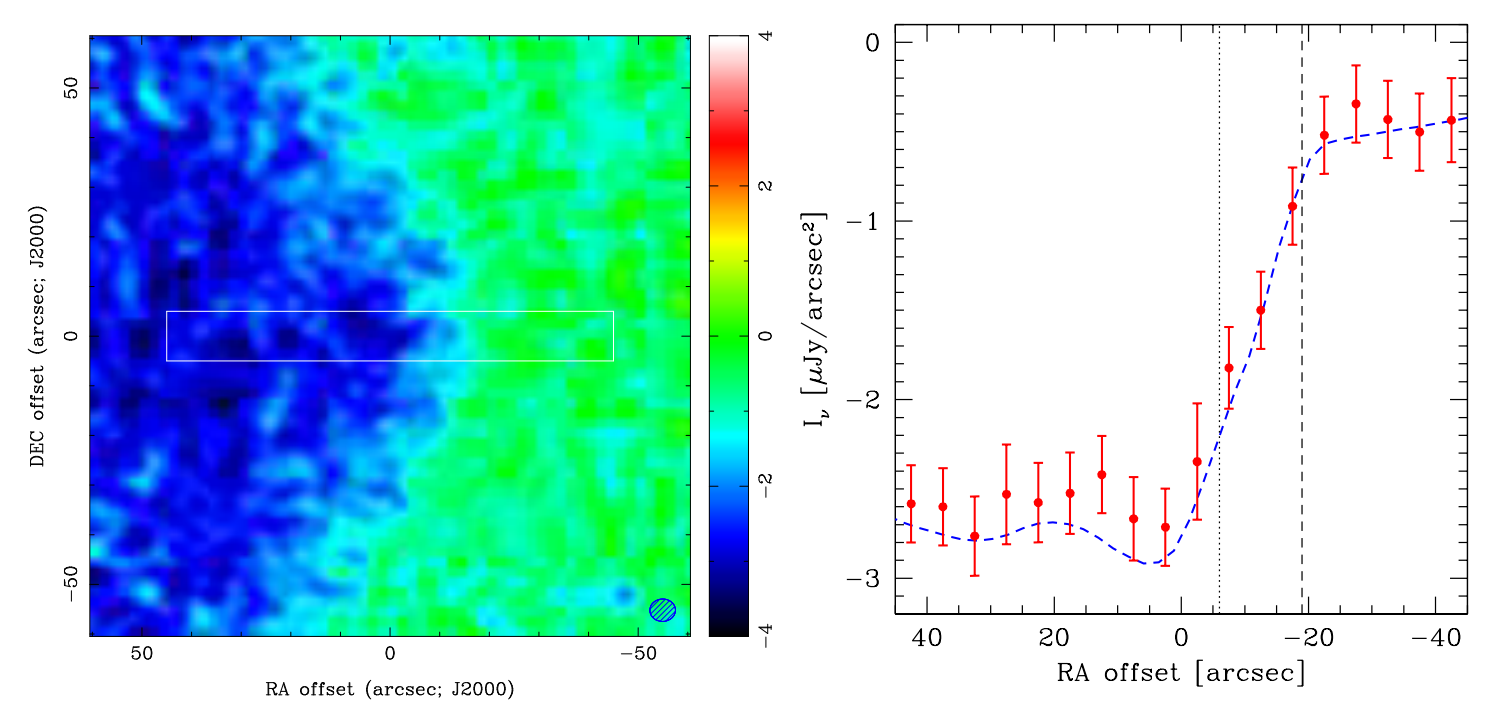
\includegraphics[width=0.8\textwidth]{bulletcluster.png}
\caption[ Bullet Cluster Simulated Shock Front kSZE Detection -[\cite{Kitayama2014}]]{Left: Simulated shock from in the Bullet Cluster at z = 0.296. Right: Simulated SZE image by ALMA at 90 GHz with standard noise components. The this dotted line indicates the location of the contact discontinuity, while the thick dashed line is the location of the shock front. Error bars indicate the expected intensity through the region in the left plot white box (\cite{Kitayama2014})}
\label{fig:bulletcluster}
\end{figure}
With this method, kSZE can be used to determine the velocity field of the cluster gas in cases where the gas is both hot or cold in a shock front, without relying on high electron temperatures or densities. 

%======================================================================================
%So, there the X-ray-emitting electrons may have a cooler temperature than the invisible protons, resulting in a steeper X-ray temperature gradient towards the outskirts and, therefore, an underestimate of the total mass (Fig. 3). (see equation 16)
%Because shock heating is an important process, and both protons and electrons are involved in the process of heating and cooling, and one is more efficient than the other, by detecting the x-ray emission from electrons (which cool more quickly), the mass of the cluster is underestimated using x-rays

% Within the spread of predictions it matches best the numerical simulations that implement AGN feedback, and it presents a slightly flatter profile compared to most of the above theoretical expectations in the outerparts. (combined measurements between Planck and XMM-Newton)

(Reconstructing gravitational potentials)
	%(Knox & Peel 2002)
(Merging Clusters) 
   (Kock \& Jetzer 2004)
    
(Scaling Relations to determine cluster mass) 
	%(Benson et al. 2013 ; Rozo et al. 2010)

% Pitfalls of studying the ICM with Xrays (McNamara et al 2005; Markevitch & Vikhlinin 2007)

%for example the (1 + z)4 dimming of the X-ray surface brightness (eq. 19)
%======================================================================================
\subsubsection{Previous Cluster SZE Detections \& Advancements}

The study of SZE is not a new branch in the field of Cosmology. Some of the first SZE measurements of clusters were made back in the 1970's on the Chilbolton Observatory 25 meter telescope in England, and at the Owens Valley Radio Observatory (OVRO) in California in the 1980's (\cite{Birkinshaw1999}). These instruments provided proof that SZE was detectable in massive clusters, but the results were often conflicting, as measurements of the same source with different telescopes returned different cluster gas temperatures. These differing values were often not within error of each other, revealing a serious systemic uncertainty not accounted for in the analysis. At the time, so few clusters were being targeted for SZE research that it was impossible to make any global statements about the properties of the intra cluster medium, or to determine the cause of the uncertainty in the measurements. 

SZE research improved with the advent of more tailored instrumentation, and an increase in the number of clusters studied. Research into the thermal effect is now extremely common in cosmology, because of its relatively high signal compared to kSZE [\cite{Benson2013},\cite{Saliwanchik2015}],\cite{Bleem2015},\cite{Planck2016}]. Most are surveys of a large number of clusters, using basic modeling of the gas, with the intent to make statistical arguments for global cluster properties. However these observations use unrefined techniques, which don't reveal any properties of cluster substructure (i.e. cooling flows, agn activity, mergers), leaving behind valuable information. This kind of study is interested in using SZE as a counting technique, to confirm cosmological parameters, and reach a lower mass detection limit for clusters at high redshift. 

Despite the ubiquity of tSZE meaurements, dedicated large scale kSZE surveys are still not realized. However, many experiments have paved the way for the TIME instrument, which will be an additional stepping block to this goal. An early example is SuZIE II, one of the first experiments to claim a 95\% confidence limit constraint on bulk flows at intermediate redshift of \(<\) 1410 km/s, in the direction of the CMB dipole. SuZIE II was a bolometer with 3 photometer bands between 150-350 GHz, which included electronic differencing of similar row and frequency bolometers, for removal of common mode atmospheric emission. The atmosphere was further removed by creating models of the observed cluster and fitting the profile to the source, subtracting any additional signal. 

Results from observing 6 clusters showed an average peculiar velocity of 150 (+430,-390) km/s , which is not a statistically significant result [\cite{Benson2003}]. In subsequent analysis, it was discovered that the results were heavily affected by differential atmospheric emission, which was not subtracted effectively by either of the above methods, leading to a modified 68\% certainty in the results [\cite{Mauskopf2000},\cite{Carlstrom2002}]. The atmospheric templates were dependent on the modeling of the cluster gas, with particular sensitivity to the distribution and temperature. SuZIE II also had large beam sizes which meant low resolution, and the inability to mask point source contamination without sacrificing large fractions of data. 

In a following data release, the total clusters observed by SuZIE II increased to 15, with additional analysis of the SZ flux and central Comptonization parameter. The data was also compared with X-ray data, and a pointed effort was made to vary the assumed beta model, investigating contributions to systematic error. This led to two important insights; that combining x-ray data with SZE signals could improve the results, and variations of the standard Beta model used in determining cluster temperatures radically changed the results. The traditional beta model is given by 
\begin{equation}
    n_{e}(r) = n_{e0}(1 + \frac{r}{r_{c}}^{2})^{-3\beta/2}
\end{equation}
and is a measure of the radial electron number density of the cluster. This changes the projected radial dependence of the Compton parameter as follows
\begin{equation}
    y(b) = y_{0}(1 + \frac{b}{r_{c}}^{2})^{1/2 - 3\beta/2}
\end{equation}

Central Comptonization is similar to the Compton Y parameter, but is applied at the center of the cluster, and depends on the electron density and temperature. The cluster centroid was determined using X-ray data from ROSAT, which included published models of gas density and electron temperature. However, those variables are sensitive to other processes within the cluster, such as cooling flows, increasing the measurement uncertainty. When two different models were fit against the data for cluster A1689, the calculated central comptonization changed by 40\% [\cite{Holzapfel1997b}, \cite{Reese2002}]. This was because the cluster was poorly resolved by SuZIE II, and relied entirely on the assumed ICM gas model [\cite{Benson2004}]. 

Other instruments followed SuZIE II to make improved kSZE measurements of individual clusters, including Z-Spec. Rather than relying on photometry, Z-Spec utilized an R \~ 300 grating spectrometer between 185 - 305 GHz to make measurements of a single cluster RX J1347.5-1145. The retrieved kSZE spectrum revealed a non-uniform fit to the gas template, consistent with X-ray detected shock regions to the southeast of the cluster center. This combined with variations in the cluster shape led to difficulty in constraining an optimal isothermal beta model, since shocks and non-uniform structure change the clumping and temperature of the ICM gas. The team reported that if the beta model was changed to those used in other literature, the Compton Y value would change as much as 25 \%. The issue of beta model dependancy is a standing problem for SZE research, and will have to be addressed again for TIME.

Z-Spec also highlighted additional uncertainties in the data, in particular, that of foreground sub-mm sources. A simulation was run with several foreground galaxies fed through the Z-Spec data pipeline for a random patch of sky, with changes in the continuum background flux reported next to the kSZE. The change in the background had a mean near zero, but a bias as large as 300 $\nu Jy$ if a source were in the beam. Most analysis performed for kSZE assumes that the sub-mm background is well understood. However that assumption may not hold if the cluster is significantly lensed, and could cause problems for large scale kSZE surveys of the future [\cite{Zemcov2012}].

Each instrument presented so far has reported some dependence on the beta model, and also had differing beam sizes. TIME will also share these traits, which is why research into this dependence is vital to understanding data results. Investigations made by \cite{Saliwanchik2015} et al. discovered that the optimal beam size for least dependence on the gas model was one the same size as the cluster. This result was obtained by first creating a simulated universe based on current cosmology, and populating it with realistic CMB background fluctuations, sub-mm clusters, radio point sources, and others. Any of the clusters created were given a standard isothermal beta profile, and were then ``measured'' in the same way as the South Pole Telescope (SPT) performed observations. The beam size across the cluster was allowed to vary, and the recovered profiles of the cluster, namely the calculated Compton Y parameter was compared to the one inputted by the simulation. The calculation is similar to the one employed by the SPT, where the source function of the SZE signal is integrated over some finite area

\begin{equation}
Y_{SZ} = 2\pi \int_{0}^{\Theta_{int}} S(\theta) \theta d\theta
\end{equation}

where $\Theta_{int}$ represents the angular aperture of the beam. Since the source template for the cluster was a perfect 2 dimensional projected $\beta = 1$ model, given by $\Delta T = \Delta T_{0}(1 + \theta^{2}/\theta_{c}^{2})^{-1}$, this integral has a simple analytical solution with familiar quantities. 

\begin{equation}
Y_{SZ}^{\theta} = \frac{\pi \Delta T_{0} \theta_{c}^{2}}{f_{x} T_{CMB}} Log[1 + (\frac{\theta}{\theta_{c}})^{2}]
\end{equation}

$f_{x}$ is the equation for the relativistically corrected canonical SZE given by 
\begin{wrapfigure}{r}{0.55\textwidth}
\vspace{-0.8cm}
  \begin{center}
    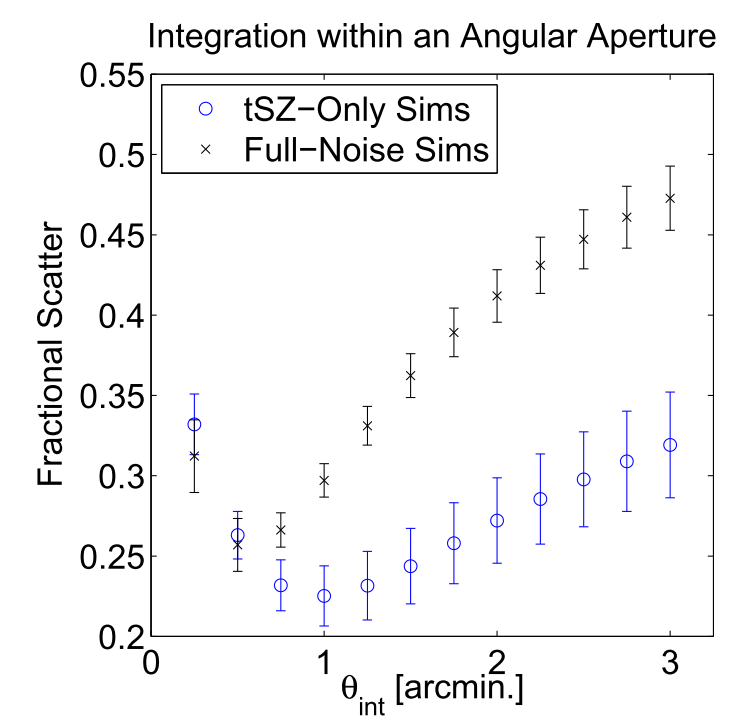
\includegraphics[width=0.5\textwidth]{saliwanchick1.png}
   \end{center}
\caption[MCMC Cluster Simulation Showing Scatter Versus Integration Angle -(\cite{Saliwanchik2015})]{The tSZE only simulation contains intrinsic scatter of the dataset. The full scatter set includes the CMB, point sources, atmospheric, and instrumental noise. This was a simulation for clusters at a median redshift of $z = 0.6$ (\cite{Saliwanchik2015})}
\label{fig:sali1}
\end{wrapfigure}
relativistically corrected SZ spectrum, $T_{CMB}$ is the temperature of the CMB background at 2.73 K, while $\delta T_{0}$ is the central temperature decrement compared to the CMB. Pipeline and real data were then compared to known scaling relationships for calculating scatter, using both tSZE only and tSZE + Noise measurements. The results shown in Figure ~\ref{fig:sali1} clearly indicate that the least scatter from the retrieved data set is for beam sizes equivalent to the angular diameter of the cluster at the given redshift (or \(\theta_{int} = 1\)). TIME is still in the process of selecting optimal cluster candidates, but this additional factor will be taken into consideration to relieve some modeling uncertainty.  

While the research above used standard cosmology to determine the effect of beam size on the kSZE signal uncertainties, conversely other groups made efforts to use large kSZE surveys to constrain the standard model. \cite{Hand2012} were not able to made significant measurements for the velocities of individual galaxies (the ultimate goal), but they were able to infer a mean pairwise momentum from low significance kSZE data. They were also one of the first groups to make any statistical arguments from a large group of kSZE detected clusters. This was made possible through arcminute resolution maps from the Atacama Cosmology Telescope (ACT), which measured an effective microwave temperature at 148 GHz due to the kSZE. The signal is a noisy estimator of the cluster line of sight momentum in the direction of the cluster. This was combined with data from the Sloan Digital Sky Survey III (SDSS- III) Baryon Oscillation Spectroscopic Survey (BOSS), providing the locations and spectroscopic redshifts for the same clusters. 

The statistic for calculating the mean pairwise momentum due to the kSZE is as follows.
\begin{equation}
    \tilde{p_{kSZ}}(r) = - \frac{\sum_{i < j}[(T_{i}-\tau(z_{i})) - (T_{j}-\tau(z_{j}))]c_{ij}}{\sum_{i<j}c^{2}_{ij}}
\end{equation}
In order to remove redshift dependencies (infrared galaxy emission, tSZE signal evolution with cluster mass), the average microwave temperature was found for clusters at the same redshift, given by $\tau(z_{i})$ above, and was smoothed with a Gaussian. 
\begin{wrapfigure}{r}{0.55\textwidth}
  \vspace{-0.8cm}
    \begin{center}
      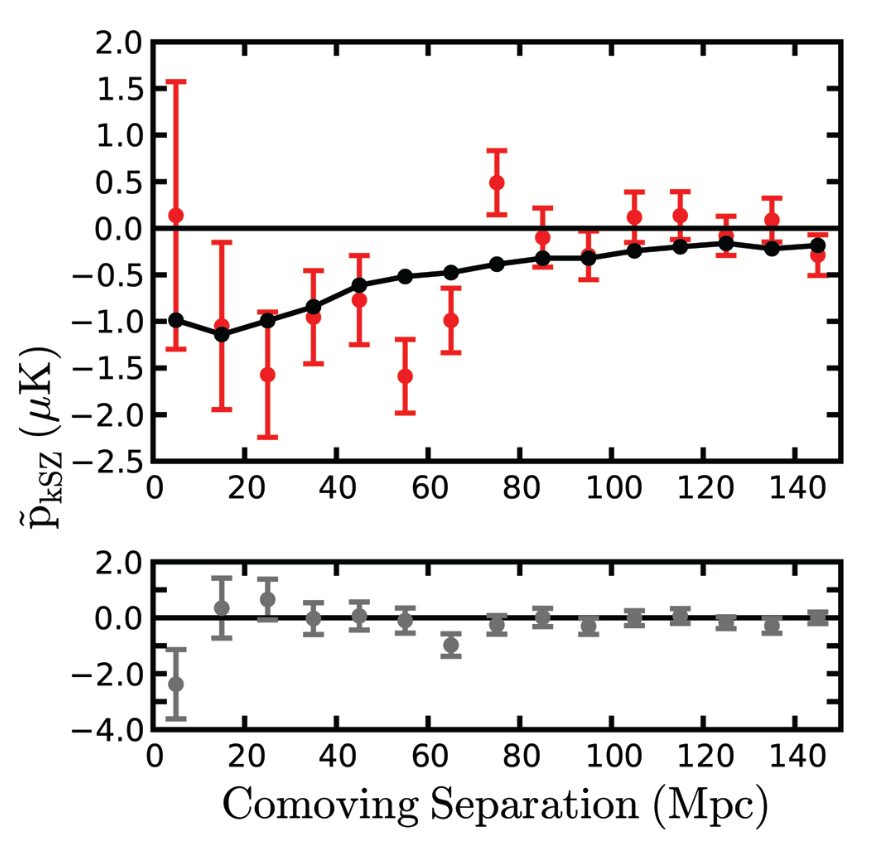
\includegraphics[width=0.5\textwidth]{hand1.png}
    \end{center}
\caption[Mean Pairwise Momentum of BOSS DR9 Selected Clusters using kSZE -(\cite{Hand2012})]{TOP: Mean pairwise kSZE signal for the 5000 most luminous BOSS DR9 galaxies in the ACT sky region, as well as a simulation for comparison. The real data set is shown in red, while the simulation, based off of large-volume cosmological simulations, is shown in black. The red data points were corrected for any redshift dependent temperature contributions, and minimizes the total Poisson and pixel noise. Errors were estimated using bootstrap resampling. BOTTOM: The probability of data given a null signal, consistent with a null signal. [\cite{Hand2012}]}
\label{fig:hand1}
\vspace{-0.4cm}
\end{wrapfigure}
This was subtracted from the kSZE calculated temperature of $T_{kSZ} = - N_{kSZ} p_{i} \cdot \hat{r_{i}}$, where $N_{kSZ}$ is a normalization factor accounting for the size of the beam, pixel scale, and cluster density profile. $T_{kSZ}$ is only an acceptable statistic if it is assumed the ratio of the total cluster mass to its mass in hot gas is the same universal ratio of matter to baryon density. 

The statistic was then plotted against a simulated kSZE signal generated by a standard $\Lambda CDM$  cosmology and simulated sub-mm galaxies and background.
The result is shown in Figure \ref{fig:hand1}, and shows a measurement of the cosmic velocity field made directly with respect to the rest frame of the universe [\cite{Hand2012}]. 
\begin{wrapfigure}{r}{0.55\textwidth}
  \vspace{-0.8cm}
    \begin{center}
      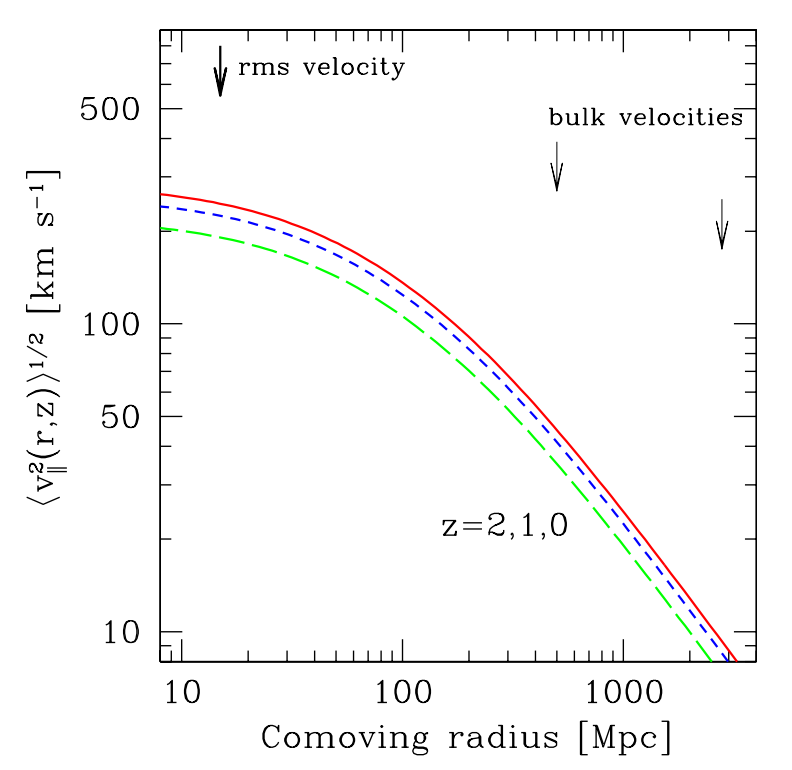
\includegraphics[width=0.5\textwidth]{kitayama1.png}
    \end{center}
\caption[Planck constraints on bulk flow -[\cite{Kitayama2014}]{Planck bulk and rms velocity measurement upper limits (\(2\sigma\)) compared to predictions using linear theory evolution of matter power spectrum. The red line is for z = 0, blue is z=1, and green is z=2 for standard \(\Lambda CDM\) cosmology.  [\cite{Kitayama2014}]}
\label{fig:bulkflow}
\vspace{-0.8cm}
\end{wrapfigure}
The authors noted that this result fits with the standard cosmology, but the data points leave significant room for improvement, and is not completely conclusive. Another caveat to the result is that the statistic used is differential, making it less sensitive to systematic effects, but also not allowing for a direct measurement of bulk flow.  

Direct measurements of bulk flow have been accomplished by several groups using kSZE, but with varying results. Several groups have found values that are far larger than that predicted by \(\Lambda CDM\) cosmology (\cite{Kashlinsky2008},\cite{Watkins2009},\cite{Lavaux2010}). Figure ~\ref{fig:bulkflow} shows the predicted velocities calculated with Equation \ref{eq:bulkvelocity} above, compared with measurements taken by Planck. Values are given as upper limits, but are still significantly higher than those predicted. It should be noted, however, that bulk flow estimates have been reported at higher values when determined through a numerical simulation than the given equation (\cite{Kitayama2014}).

Some theories have been developed to try and explain these results. One is that somehow the gravitational attraction of baryonic matter was strengthened at late times (matter dominated era), speeding up structure formation and increasing peculiar velocities. One group ran an N-body simulation under these conditions and found that at scales  \(R > 100\) \(h^{-1} Mpc\) , bulk flow velocities increased by roughly \(40\%\) compared to \(\Lambda CDM\) cosmology (\cite{Wyman2010}). Another theory is that there exists an instrinsic dipole in the CMB caused by superhorizon fluctuations in the scalar matter fields, prior to inflation. This would cause an increase or decrease of the bulk flow depending on the location of the cluster (\cite{Mak2011}).  What all explanations have in common is that they reveal inconsistencies in the standard model that are due to real, unknown physical phenomenon, and not from measurement error. 

While all are certainly possible, it has been extremely difficult to narrow the options because of small counting statistics. This is in part due to the small number of clusters in the relatively nearby universe (100-200 \(h^{-1} Mpc\)) (\cite{Lavaux2013}), and the limited size of most kSZE surveys. TIME will not be able to create a large survey of kSZE, but by improving detection techniques and increasing the sensitivity of high redshift signals, it will improve the statistical significance of bulk velocity measurements, and increase the total number of clusters measured. Further constraints on the standard model will then be possible.  

\subsubsection{Foregrounds \& Backgrounds for TIME SZ Measurements}

Outline:
\begin{itemize}
    \item astmospheric contamination on different scales
    \item simply mention that we have a way of isolating the atmospheric time varying signal in frequency space and removing that from the data
    \item 
\end{itemize}

One of the improvements that TIME will seek to make is in modeling atmospheric noise. While SuZIE II suffered from differential atmospheric contamination, TIME will have dedicated monitoring channels that will sample both on and off the cluster. This should help remove any time varying atmospheric signal from the data.


The TIME instrument has a field of view on the scale of arcminutes, which is the limiter for the smallest and largest modes it is sensitive to. For the atmosphere, fluctuations at the largest spatial scales will impact bolometer data at the highest frequencies. Often, instruments will have data pipelines with high or low pass band filters that will cut out the unwanted noise above or below a critical frequency respectively. But this kind of aggressive chopping has downsides. For Bolocam, another bolometric SZE instrument similar to TIME, a high pass filter was applied to remove large angular scale atmospheric fluctuations, but it had the negative side effect of removing part of the SZE signal, also on large angular scales. If the atmospheric emission varies on scales equal to the size of the cluster, then significant portions of SZE data are lost by this method. The only way that the data could be recovered was through spatial modeling of SZE, and comparing it to the remaining data set using a parametric fit. Missing data from the instrument, but present in the model, could be added back in, but with significant biases [\cite{Sayers2013}].

%"Background radiation is radio frequency radiation that originates from farther away than the object being studied, whereas foreground radiation originates from closer than the object being studied."

%================================================================================================================
While atmosphere is one foreground common for millimeter wave observations, a background to consider is dust emission.
\begin{wrapfigure}{r}{0.55\textwidth}
\vspace{-0.8cm}
  \begin{center}
    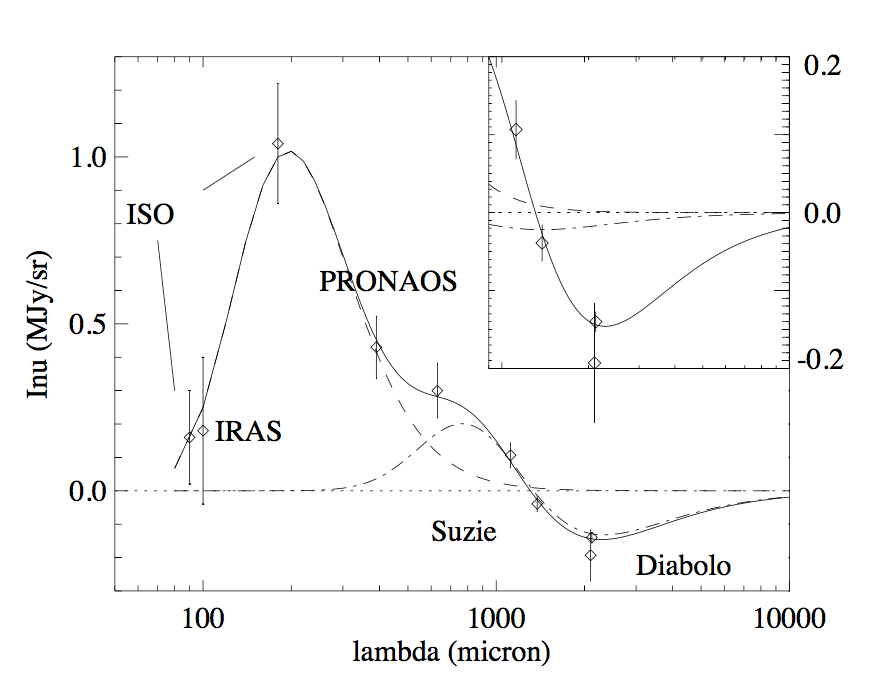
\includegraphics[width=0.5\textwidth]{birkinshaw1.png}
   \end{center}
\caption[TIME's frequency window will be mostly free of dust emission contamination. -(\cite{Birkinshaw1999})]{Measurements of Abell 2163 from mm to far-IR by multiple instruments. The solid line is a best-fit model for combined dust emission and SZE. The dash-dotted line is tSZE, while the dashed line is the isolated dust contribution. The dust emission falls off completely after $\sim$ 1000 microns [\cite{Birkinshaw1999}].}
\label{fig:dust}
\end{wrapfigure}
In Figure \ref{fig:dust}, the isolated dust contribution for SZE measurements of Abell 2163 is shown. Dust emission falls off completely before 300 GHz, only slightly within the outer limits of the TIME high frequency band (183-326 GHz). 

%================================================================================================================
The next noise contributor that must be taken into account is sub-mm point sources. A common problem with early instruments was a low resolution, incapable of distinguishing between the cluster and contaminating foreground galaxies. Massive clusters are rich environments for many different types of phenomena, including dusty galaxies and lensing contamination, which can radiate heavily in the radio to sub-mm portion of the spectrum. If the resolution is poor, the radio contamination would be misconstrued as the actual SZE signal for the cluster. With the angular resolution of TIME, the cluster contaminating sources can simply be removed from the offending data cube ``pixel'' and fitted with a smoothing function to reduce signal averaging errors. 
%================================================================================================================

Intrinsic to this frequency range is also the ability to isolate the kSZE signal to high significance. In the left graph of Figure \ref{fig:tksze}, it was shown that for most frequencies, the kSZE signal is so faint that it is virtually impossible to detect for a high redshift cluster, if the tSZE signal is present. If the Kompaneets Equation presented above is examined more carefully, it can be seen that the tSZE has a null at 218 GHz, directly in the spectral range of TIME. This value can shift slightly for clusters with large numbers of relativistic electrons, as shown in the right graph of Figure \ref{fig:tksze}, but the effect is minimal. 

This result takes into account the background and foreground noise sources mentioned above, as well as the differential atmospheric removal technique. The expected measurements of kSZE for TIME are shown in Figure \ref{fig:time1}. TIME's sensitivity will easily reach kSZE intensities for a massive cluster at $v_{pec} = 1000 km/s$, and extend to clusters below that velocity.

\vspace{30.0cm}
\hspace*{-0.8cm}
\begin{figure}[H]
\centering
\captionsetup{width=\textwidth}
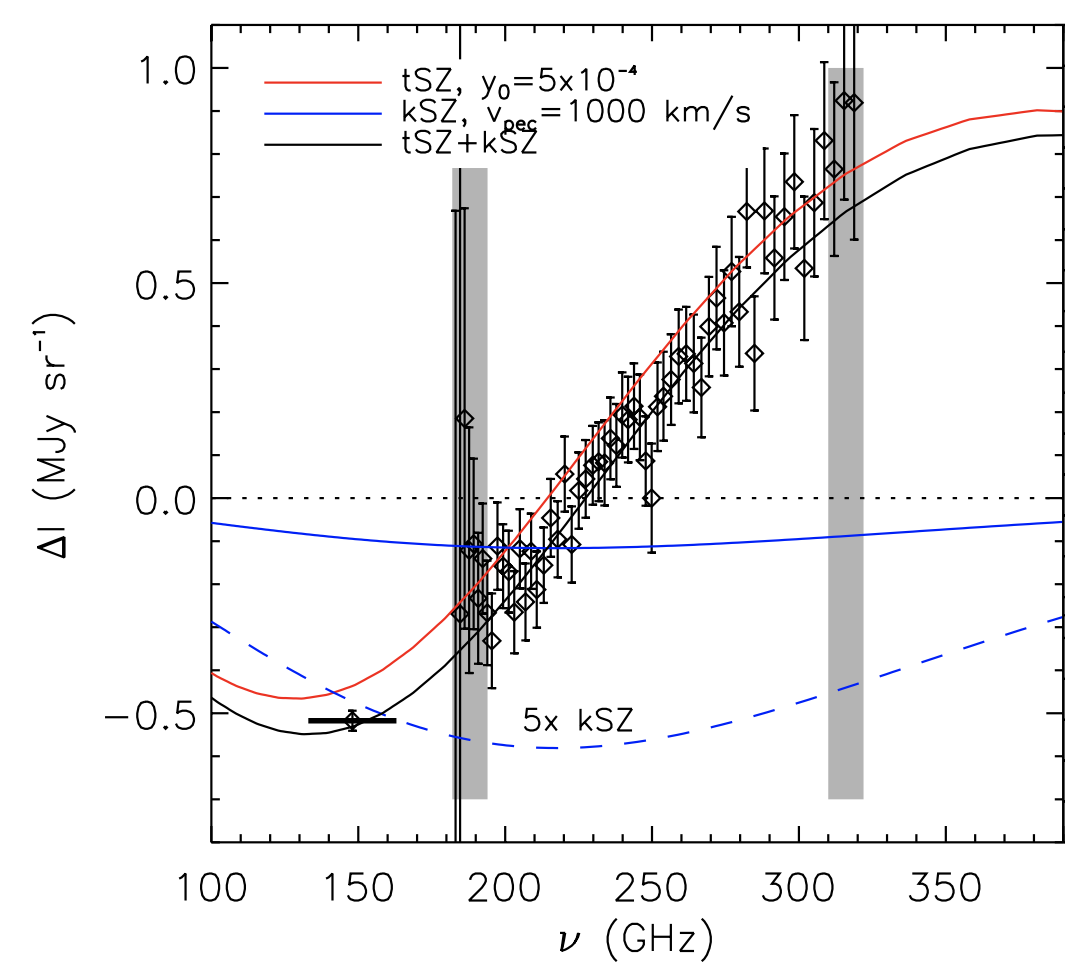
\includegraphics[width=\textwidth]{time1.png}
\caption[Expected TIME kSZE \& tSZE Measurements]{Simulated measurements of tSZE and kSZE with TIME. Grey bands are atmospheric monitoring channels. The solid and dashed lines are theoretical calculations of the effect using the equations given in the science discussion above, while the diamonds are the estimated performance for TIME. This estimated detection assumes astrophysical contamination, the atmospheric subtraction method described above, and assumes 10 hours of observation on the cluster.}
\label{fig:time1}
\end{figure}

%============================================================================================================
\newpage
\section{TIME Hardware Overview}
\subsection{Transition Edge Sensor Bolometers}
Following in the footsteps of previous instruments, TIME will utilize Transition Edge Sensor (TES) Bolometer technology to attain the previously mentioned science goals. Bolometers perform a different function from detectors used at shorter wavelengths, which typically count photons through their interaction with an absorber material (CCD, CMOS). A photon at visible light wavelengths, for example, has a high enough energy to excite electrons within a doped material, which gets recorded as current. Radio wavelength photons have such low energies that any signal on a CMOS device would be insignificant compared to the dark current. Rather than forcing a photon to transfer its energy, a bolometer material simply absorbs it, and experiences a temperature change.

This makes a bolometer a sophisticated thermometer, but one which uses the resistance in an electrical circuit to measure the temperature of a thin, metal-mesh absorber. The resistor typically used is referred to as a thermistor which has well characterized changes in resistance with changes in temperature. The one used by TIME is an elemental titanium thermistor with a critical temperature at \(T_{c} = 450 mK\) and \(250 mK\) base temp (\cite{Crites2014}). These two elements are then coupled to a heat sink, which provides a base temperature against which to compare the absorber temperature. Once a photon strikes the detector, the temperature changes minutely, the thermistor drastically changes in resistance, and the voltage across the circuit decreases. The voltage across the bolometer is initially biased by pre-amplifying superconducting quantum interference devices (SQUIDS) (see section 3.3), and ensure that any change in power induced by photons is countered. This keeps the total loading power constant, and within the efficient superconducting transition. Since the SQUID bias is a well known value, and the total power is constant, the power induced by the photon can be determined (\cite{O'Brient2010}).

\begin{figure}[H]
\centering
\captionsetup{width=0.9\textwidth}
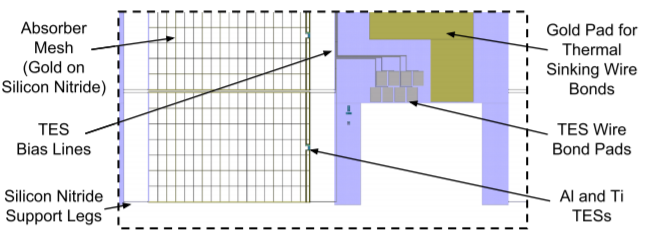
\includegraphics[width=0.9\textwidth]{jon5.PNG}
\caption[Single TES Detector Pixel -(\cite{Hunacek2016b})]{A close up diagram of a single bolometer mesh absorber pixel. This is one of 80 pixels in the high frequency detector subarray shown in Figure~\ref{fig:jon4} (small gold squares) (\cite{Hunacek2016b})}. 
\label{fig:jon5}
\vspace{-0.8cm}
\end{figure}

TES bolometers have some advantages over a normal superconducting bolometer which make them ideal for mm-wave research. For one, it has a typical resistance around \(1\Omega\), making it very robust to vibrational pickup. This is due to the voltage being biased into a normal superconducting transition, which has the added advantage of rapid changes in resistance, but small changes in temperature. The detectors are also fabricated by lithographing and etching of thin films, allowing for large and densely packed arrays at a low cost (\cite{O'Brient2010}). A small portion of a TIME prototype array is shown for clarity in Figure~\ref{fig:jon4}.

TIME will have a total of 1840 TES Bolometers organized into 48 detector sub arrays split into 72 low frequency and 80 high frequency detectors. Figure~\ref{fig:jon4} shows the detector module fabricated on silicon wafers, a gold plated aluminum holder, which is connected to a readout circuit board with cabling (\cite{Hunacek2016}). A single detector pixel is gold suspended on a released silicon nitride web, which absorbs radiation from the spectrometers, and is connected to thin silicon nitride legs coupling it to the 250 mK bath (see Figure~\ref{fig:jon5}). Significant difficulties arose from attempting to keep the web suspended during normal operation with as few legs as possible, but it was found that a 250 mK bath was more than adequate to allow suspension legs 4 times thicker than average. This allowed the same saturation power without adding phonon noise, and improved the device yield and durability (\cite{Hunacek2016b}). The expected efficiencies and performance for both halves of the detector module are provided in the table below.

\begin{figure}[H]
\centering
\captionsetup{width=0.9\textwidth}
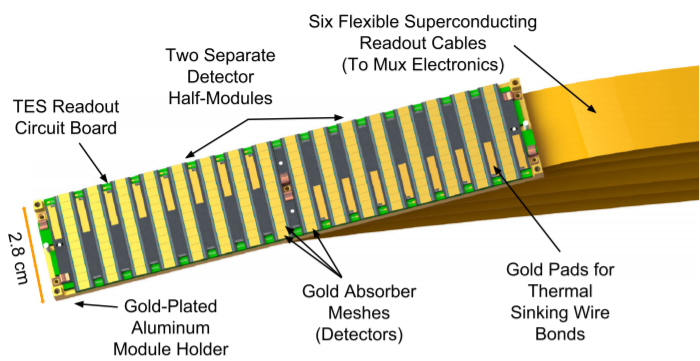
\includegraphics[width=0.9\textwidth]{jon4.PNG}
\caption[Diagram of a Half Detector Module -(\cite{Hunacek2016b})]{Half detector wafer module (high frequency) and superconducting readout cables. Each module hosts 12 spectral pixels indicated by gold squares. Green squares show silicon cutouts to expose the circuit board to which the TES bias lines are bonded (\cite{Hunacek2016b}).}
\label{fig:jon4}
\end{figure}

\begin{center}
    \begin{tabular}{|c|c|c|c|}
    \hline
    \multicolumn{4}{c}{TES Bolometer Parameters} \\
    \hline
    \hline
    Parameter & Photometers & Grating LF Band & Grating HF Band \\
    \hline
    TES safety factor ($P_{elec}/P_{opt}$) & 2.5 & 2.4-2.8 & 2.1-5.1 \\
    Detector + MUX NEP [$10^{-18} W Hz^{-1/2}$] & 40 & 9.7 & 13 \\
    Photon NEP [$10^{-18} W Hz^{-1/2}$] & 60 & 23-26 & 26-43 \\
    Absorber Size [mm] & 4.0 & 3.0 x 3.48 & 3.0 x 2.32 \\
    Spectral Range [GHz] & 135-165 & 183-230 & 230-326 \\
    Estimated end-to-end optical efficiency & 0.3 & 0.3 & 0.3 \\
    Num of Bolometers per sub-band & 1 & 24 (8x3) & 36 (12x3) \\
    Frequency Resolution per Detector & 5 & 92-122 & 90-120 \\
    NEI on sky per detector [(MJy/sr)$\sqrt{s}$] & 0.44 & 4.7-5.8 & 7.3-15.2 \\
    NEFD on sky per detector [mJy$\sqrt{s}$] & 6.7 & 84-105 & 101-131 \\
    \hline
    \end{tabular}
\end{center}

\subsection{Curved Grating Spectrometers}
TIME will also collect spectral information of the field of view (FOV) by coupling the bolometer arrays to two banks of curved grating spectrometers, each of which can handle a single polarization, at an R = 100 resolution. A single feedhorn on the grating input couples to 60 bolometers. Combined, the two banks will store 1920 total detectors divided into 6 blocks, and covering 8-12 spectral pixels  (\cite{Crites2014},\cite{Hunacek2016}). The total expected spectral coverage will range from 183-326 GHz, with each channel width at 2-3 GHz, and added edge channels for atmospheric noise reduction. The resulting on-sky array will be 16 x 1 spatial pixels spanning an instantaneous FOV of 11 x 0.35 arcminutes.

The two grating spectrometers are machined and bolted aluminum assemblies with 190 facets, and a resolving power of 140-200, much lower than the detector sampling rate. Figure ~\ref{fig:jon2} shows the largest dimension of the spectrometer at 23 cm, with a front arc where 6 detector modules will sit. This output arc between the two stacks creates 6 planes at which the detector arrays are mounted, while the back arc holds the grating teeth off of which the feedhorn output is diffracted. The overall design is a drastic reduction in weight and volume compared to similar spectrometers like those used by Z-Spec (\cite{Bradford2004},\cite{Naylor2003}), show in the right of Figure~\ref{fig:jon2}.

\begin{figure}[H]%
    \centering
    \subfloat{{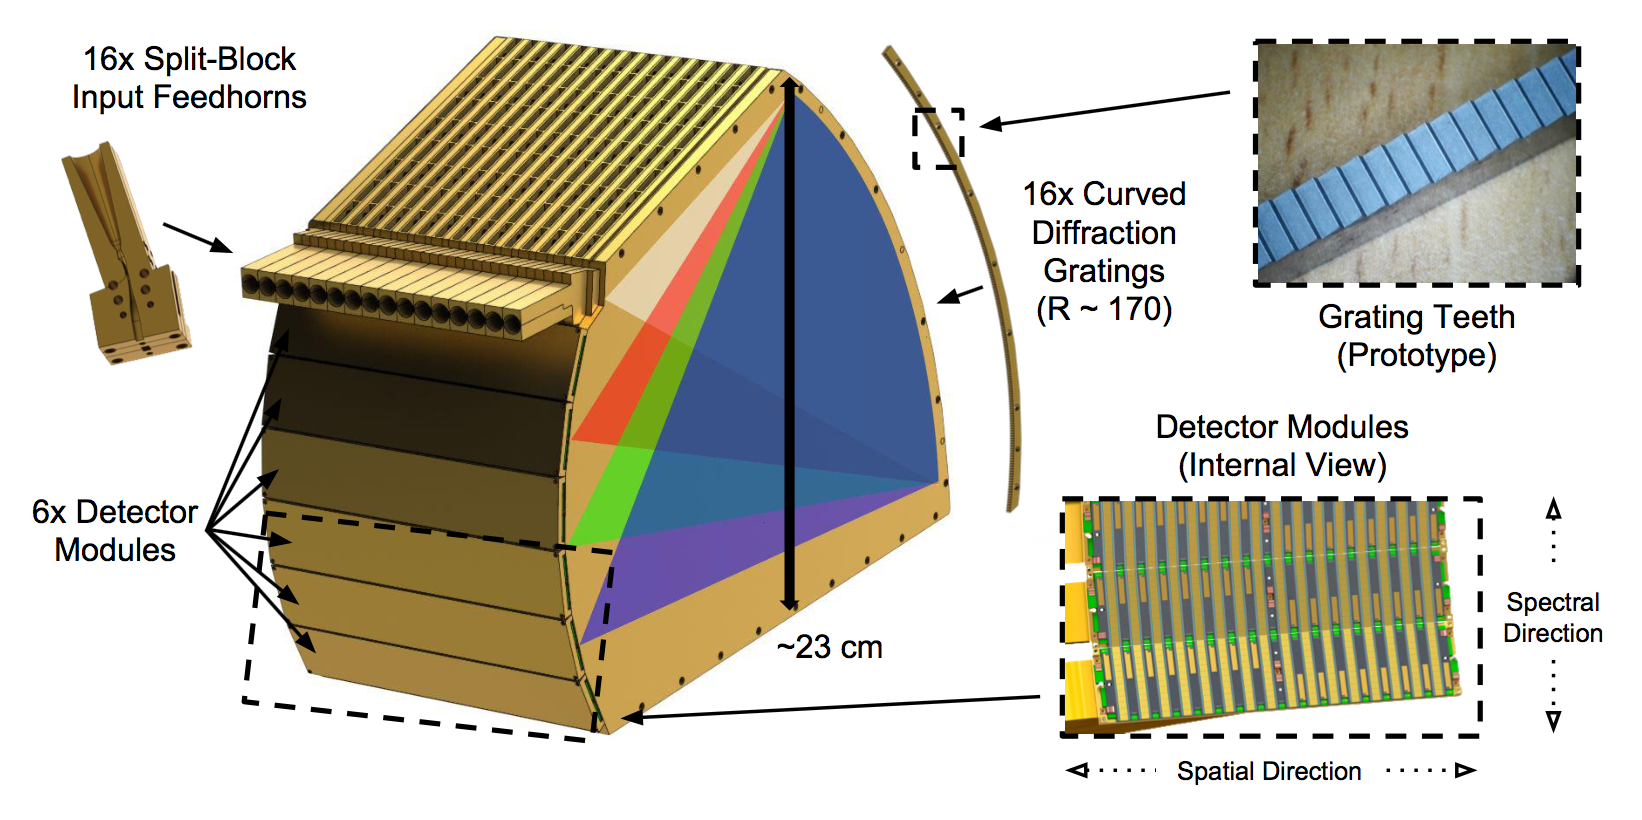
\includegraphics[width=0.6\textwidth]{jon2.png} }}%
    \qquad
    \subfloat{{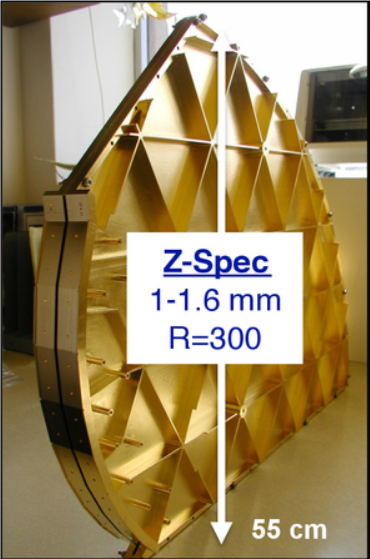
\includegraphics[width=0.2\textwidth]{abby1.png} }}%
    \singlespace
    \caption[TIME Spectrometer Banks and Detector Modules -(\cite{Hunacek2016})]{Left: Schematic of one of two spectrometer banks. The 16 input feedhorns take input from the optical path from the telescope into the cryostat, where the signal is incident on the curved diffraction gratings, and finally onto the spider mesh bolometer detector arrays (\cite{Hunacek2016}). Right: image of the Z-Spec grating spectrometer for comparison \cite{Crites2014}).}%
    \label{fig:jon2}%
    \vspace{-0.8cm}
\end{figure}
%===========================================================================================================
%===========================================================================================================
\subsection{SQUIDS}

The SQUIDS used by TIME are time-domain multiplexing (TDM) pre-amplifiers, and have several optimal characteristics that make them ideal for use with bolometers. These include low noise, low power dissipation, and a low impedence compared to typical JFET transistors (\cite{Dobbs2009}). In TDM, multiple bolometers are coupled to individual SQUIDS\footnote{In the TIME array, 40 detectors are coupled to one SQUID.} through a single wire and are biased sequentially, lightening the burden of electrical connections to the cryostat (see section 3.6). Despite these advantages, they are still subject to magnetic fields. For this reason, TIME SQUIDS are placed into a superconducting box that produces a field suppression factor of over 70 (\cite{Hunacek2016b}).

While the simplistic use of SQUIDS was given above, the actual application for this many detectors is mildly more complicated. After a photon creates a temperature change in the circuit, the thermistor shunts the induced current around a first stage of SQUIDS to a second stage where a feedback flux is provided, linearizing the first stage. This feedback signal compensates for changes in the current from the bolometers and produces a measurement of the power received by the photon. This first set of SQUID outputs is further amplified by a column of SQUIDS in series, and then read out by the Multi-Channel Electronics (MCE) (see section 3.4). Figure~\ref{fig:squids} shows the columns of SQUIDS in series connected to the first stage feedback SQUIDS. Each individual SQUID pictured connects directly to 40 detectors, because of the 40:1 multiplexing factor. The efficiency of the SQUIDS and the multiplexing functionality allows each detector to be sampled at a frequency of 20 kHz, greatly reducing the readout time compared to reading each individual detector. This frequency is also well above the chopping frequency for the detector, or the time it takes for the photon signal power to dissipate in the array (\cite{Dobbs2009}). 

\begin{figure}[H]
\centering
\captionsetup{width=0.7\textwidth}
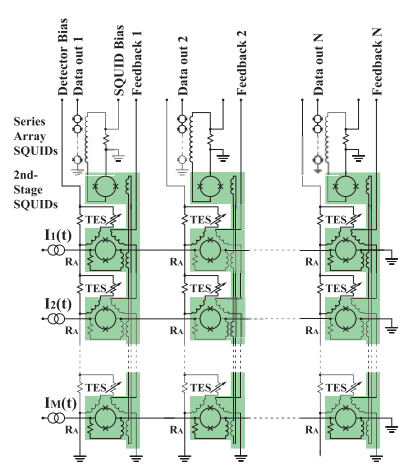
\includegraphics[width=0.7\textwidth]{squids.PNG}
\caption[Circuit Diagram for TDM SQUIDS -(\cite{Dobbs2009})]{Circuit diagram for SQUID biasing, feedback, and voltage output read by the MCE. This circuit is Time Domain Multiplexed where each 2nd stage SQUID is activated sequentially, continuously checking for detector bias changes at a 50 MHZ frequency (\cite{Dobbs2009}).}. 
\label{fig:squids}
\vspace{-0.8cm}
\end{figure}

%===========================================================================================================   
\subsection{Multi-Channel Readout Electronics System}

In order to read out the 1840 detectors, TIME will require two MCE's acting in tandem, as each one is only capable of handling 1280 pixels. The MCE has 4 readout cards (RC), one address card (AC) and one clock card (CC), all with various functions.

The address card is responsible for the multiplexing of the SQUIDs by turning on one row of SQ1's at a time, with 41 rows being revisited at a frequency of 20 kHz. The clock card (CC) is responsible for the sending and receiving of internal commands for the MCE, including requesting data from each RC, assembling the data frame, and passing the frame to the PCI card in the data acquisition computer. The CC also generates an internal 50 MHz clock in order to keep these processes time ordered, but can also take input from a Sync Box (see section 3.5) to produce a timestamp.

The 4 RC cards are the source of the most power consumption, as they perform the actual processes commanded by the CC and AC. They de-multiplex the SQUID signals for each pixel and package them into a data frame consisting of housekeeping, data, and checksum blocks. Each RC is responsible for up to 41 x 32 pixels spread over 32 output channels. They are then transferred over fiber to an external computer PCI card\footnote{It should be noted that the mapping of the SQUIDS to the detector arrays is non-trivial, and requires lab testing so that the chosen SQUID biases the correct pixel}. To view the RIT MCE components and setup used for TIME software testing, see Figure~\ref{fig:mce}.

The MCE has several operating modes designed to return different information. Low-pass filtered feedback is considered the normal mode, which returns decimated data down to a frequency of 200 Hz, to reduce the amount of disk spaced used. Mixed mode adds extra data in the form of error and feeback information to each 32-bit word recorded. For detector array characterization, it can also be set to consistent acquistion at 20 kHz or small sections of 50 MHz data. Data are processed into frames, where one data block is an array of 32x41 32-bit numbers and contains one value from each pixel. The MCE accepts user commands for defining the amount of data to be returned, whether it is a single frame of data multiple (\cite{Battistelli2008}). 

In every case above, the MCE must first go through a start-up phase that automatically characterizes the bolometer array and applies the appropriate feedback to keep the SQUIDS in a linear regime. This initial bias is applied based on a configuration file defined by the user, and is implemented for each pixel using a Proportional Integral Differential (PID) servo loop. For a full array this means processing 2100 free parameters in the span of a few minutes (\cite{Dobbs2009}).

\begin{figure}[H]
\centering
\captionsetup{width=0.95\textwidth}
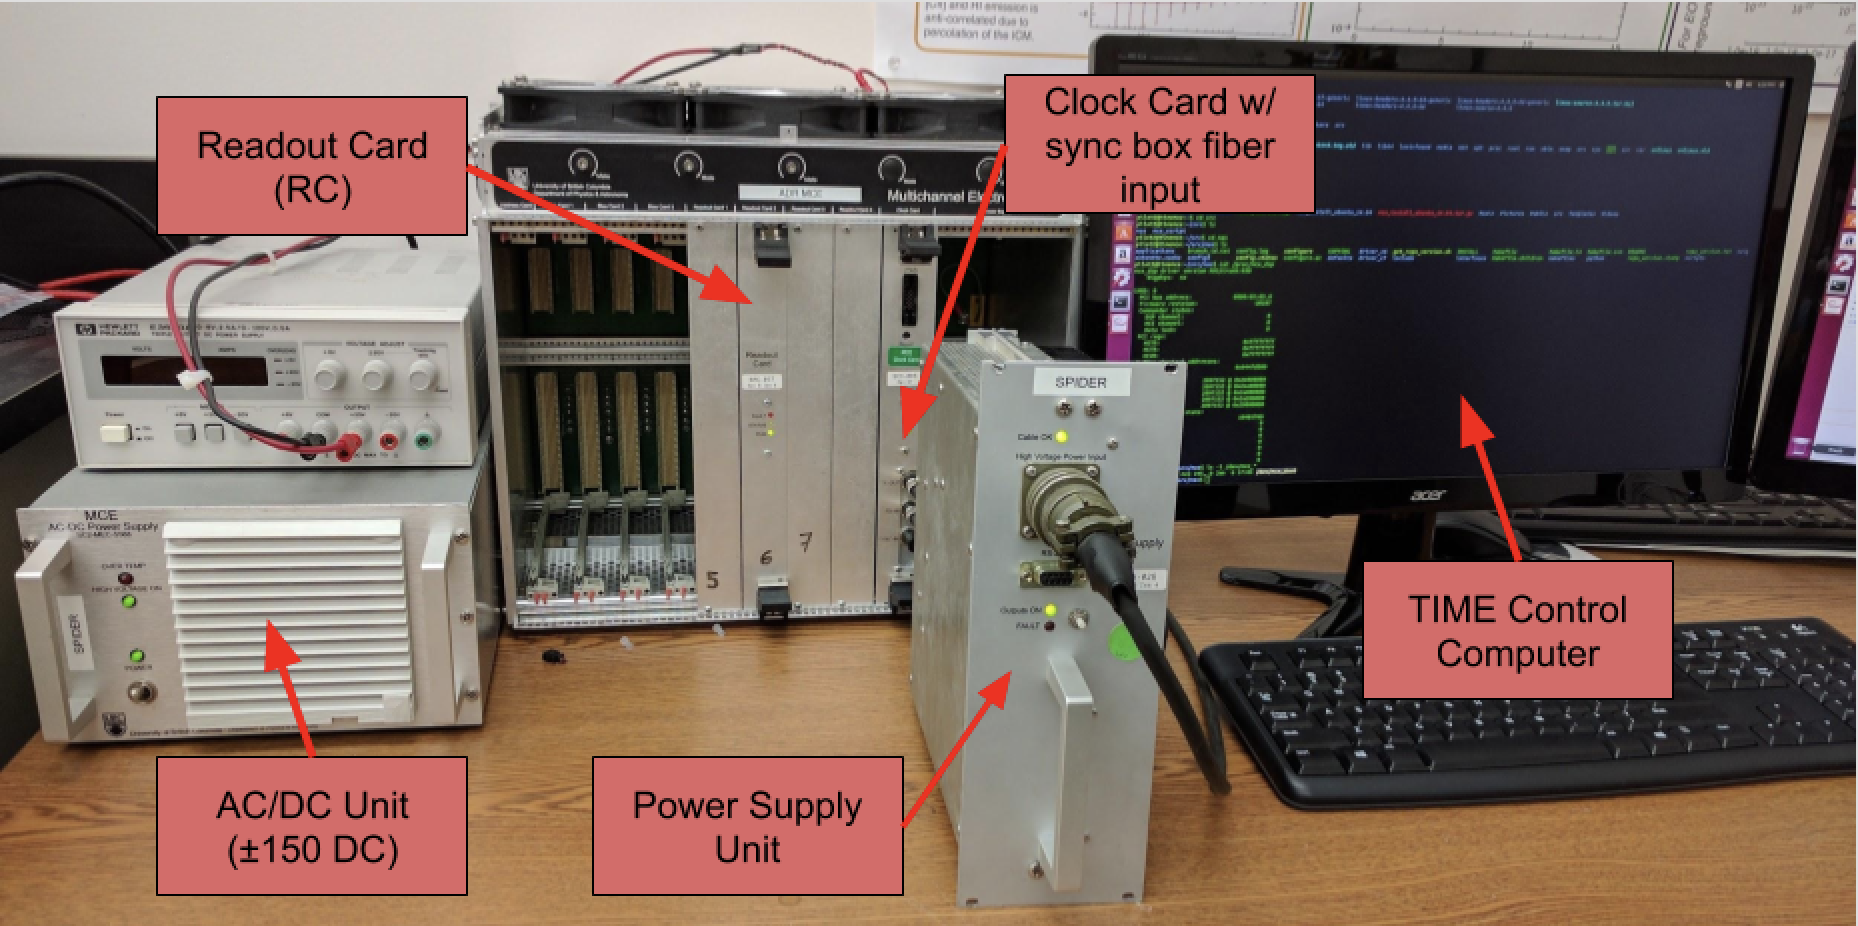
\includegraphics[width=0.95\textwidth]{timemce.png}
\caption[MCE RIT Setup with Incomplete Rack]{The setup for RIT data acquistion with one partially filled MCE rack. It contains the power supply off to the right foreground, one clock card, one address card, and one readout card. The full TIME setup will have 2 MCEs running syncronously, each with a full rack for a total of 8 RCs controlling the 1840 detectors.}
\label{fig:mce}
\vspace{-0.8cm}
\end{figure}

%==========================================================================================================
\subsection{Sync Box}
Since TIME has a large number of detectors, it necessitates the use of two MCEs, which both have an independent internal clock. When acquiring data, it is essential that both MCEs are reporting the same timestamp for each frame of data. Imagine that the detector array is a normal camera trying to take stills of a video. At each second, the image shown is completely different. If the data from each second is compared and collated as the same frame, nothing in the image would match up or be coherent. This is a similar problem for TIME, where the scan strategy forces the power incident on the detectors to vary with time. The solution to this problem is to have an external clock regulate the data acquisition for each MCE. The University of British Columbia (UBC) developed such a device apptly name the sync box. 
The sync box generates a data-valid pulse and a 32-bit number, based on a 25 MHz clock, that is sent over optical fiber to the MCE CC. This number is then added to the frame header by the CC which currently is programmed to send a random sequential integer. The sync box can control up to 8 full MCE racks, and forces the clock card in each to initiate data frame collection at the same time. The process can be thought of like an orchestra all playing to the beat of the same metronome. All MCEs wait for the sync box to supply the ready pulse before attempting acquisition, preventing any drifting of the frame times across different MCEs. This pulse is triggerable from an external source, in the case of TIME, a box that is communicating with an external Network Time Protocol (NTP) server, which provides the sync box with an atomic world clock timestamp to send to the MCE frame header. This allows data collected by other systems, namely the telescope, to be compared by timestamps in the same units, rather than arbitrary conversions done after the fact (\cite{Battistelli2008}).

\begin{figure}[H]
\centering
\captionsetup{width=0.95\textwidth}
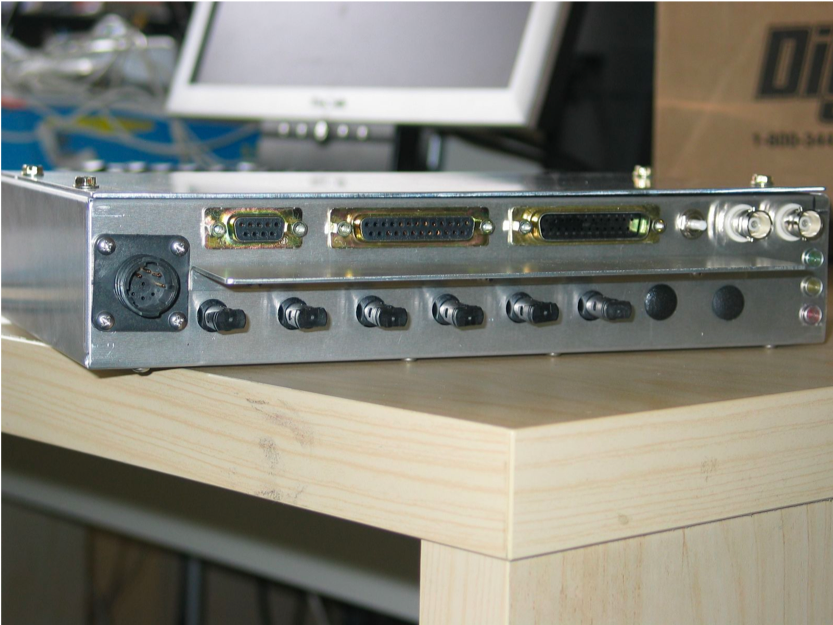
\includegraphics[width=0.95\textwidth]{sync.png}
\caption[University of British Columbia Sync Box]{A 5V DC sync box showing 6 out of the 8 possible fiber outputs for connecting to 8 MCE CCs. From upper left to right is a RS-232 command port that allows the sync box to be programmed over {\sc Minicom}, 25-pin digital I/O, obsolete DB-25M, and finally a femal BNC in/out for an external TTL clock (Taken from UBC MCE Wiki)}
\label{fig:mce}
\vspace{-0.8cm}
\end{figure}

%====================================================================================================
\subsection{Cryostat}
The TES bolometers described above are held at superconducting transitions and therefor require cooling down to hundreds of mK. To accomplish this, the spectrometer/bolometer system is housed in a closed cycle cystostat with 5 cooling stages ranging from 50 K down to a base temperature of 250 mK. These stages are shown in Figure ~\ref{fig:jon1} without the shields\footnote{The casing is custom fabricated by {\sc Amuneal} and is intended to provide magnetic shielding for the instrument}. The 50 K stage is cooled by a cryomech PT-415 pulse tube refrigerator down to 4 K, with two custom lower temperature stages; a \(^{4}He\) system down to 1 K, and a \(^{3}He\) dual sorption system for 300 mK. A second \(^{3}He\) stage creates the 250 mK required for the spectrometers. Between these stages are also several stops, filters, and supports designed to prevent leakage of the optical load from each subsequent stage. Working outside to in, a zotefoam window provides the first line of defense against stray light, followed by the 4K stage lyot cold stop at the pupil, while the 1K stage holds a final polyethylene reimaging lens with an f/3 focus, covered in a porous teflon AR coating. In addition, the 1 K and 300 mK stages have metal mesh low-pass edge filters and dielectric filters to reduce the optical loading on the final 250 mK stage (\cite{Crites2014}).

\begin{figure}[H]
\centering
\captionsetup{width=0.85\textwidth}
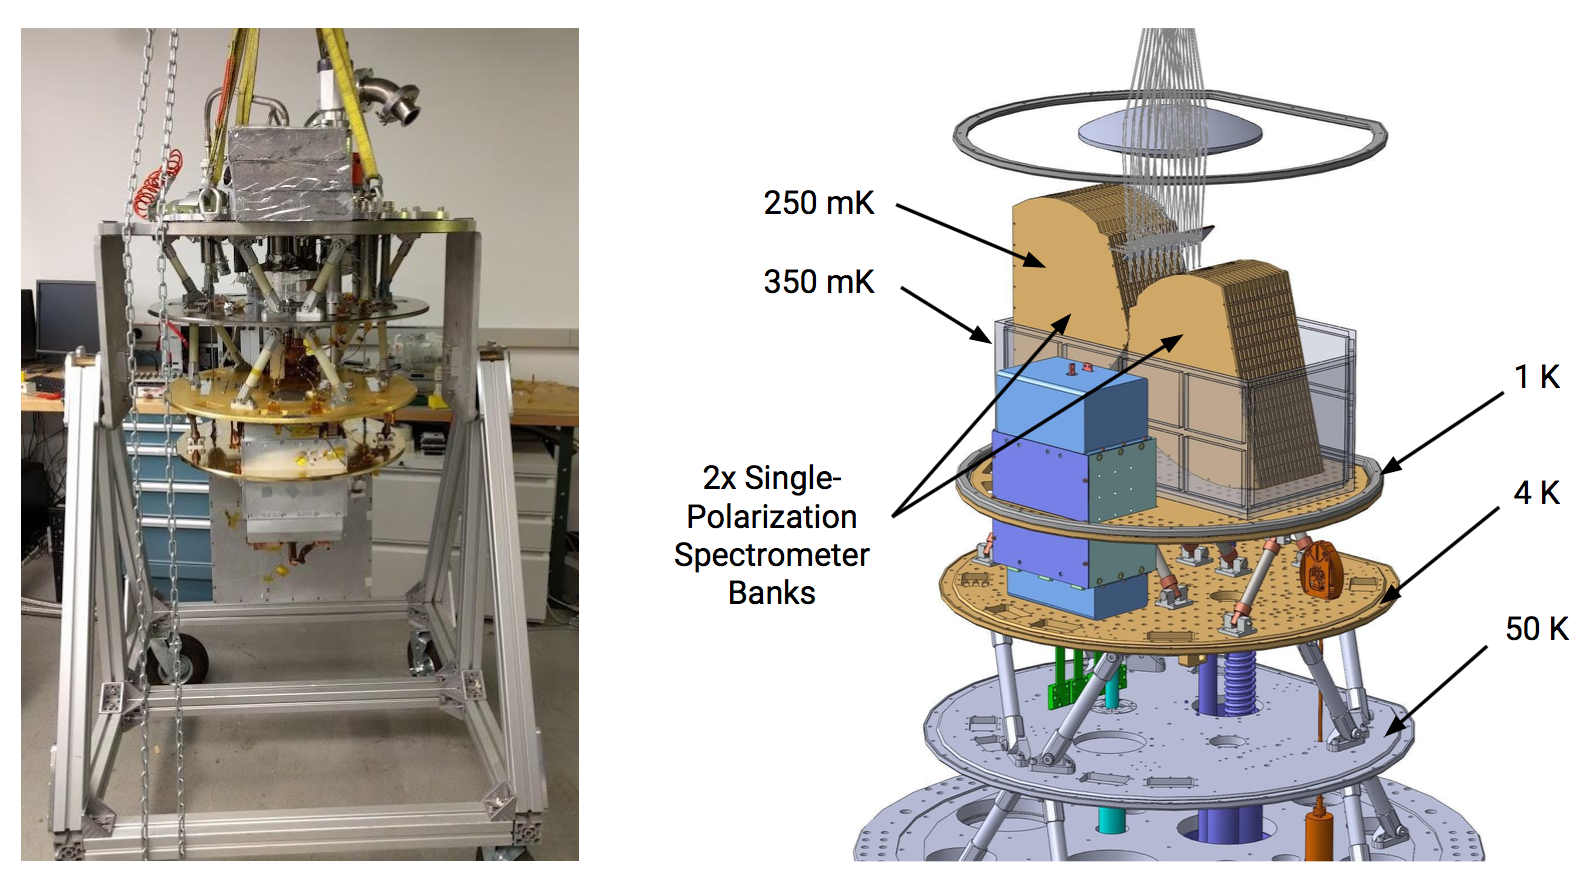
\includegraphics[width=0.85\textwidth]{jon1.png}
\caption[TIME Cryostat -(\cite{Hunacek2016})]{Left: Cryostat on support structure without shields, located in the Caltech Experimental Cosmology Lab. Right: Model of Cryostat showing placement of the spectrometer banks, various cooling stages, and overall support and shock absorptive structure. (\cite{Hunacek2016})}
\label{fig:jon1}
\end{figure}

%===================================================================================================
%===================================================================================================
\section{Optics}

The optical path into which the TIME instrument will be integrated is given in Figure~\ref{fig:optpath}, and contains three primary elements; the telescope, the K-Mirror System (KMS)(see section 4.2), and the TIME cryostat containing the cold optics. The KMS takes input directly from the telescope secondary mirror through an invar flange, which is incident on K1 in the right figure. This is reflected off of the other two aluminum mirrors K2 and K3, which dynamically rotates the image, and is passed to another mirror, F1. F1 serves to bend the optical path between the K-Mirror system and the cryostat so that it will fit within the cabin. In order to ensure that the image and pupil of the telescope reaches the cold optics of the cryostat, three powered mirrors, P1, P2 and K2 form a relay that effectively connects all three optical elements. Once the cryostat is installed in the cabin, the P2 mirror will also be used to correct the optical path between the KMS and the cryostat to ensure proper alignment. This is necessary because of the great weight of the cryostat, and the flexible carbon fiber floor of the cabin which is expected to warp.

\begin{figure}[H]%
    \centering
    \subfloat{{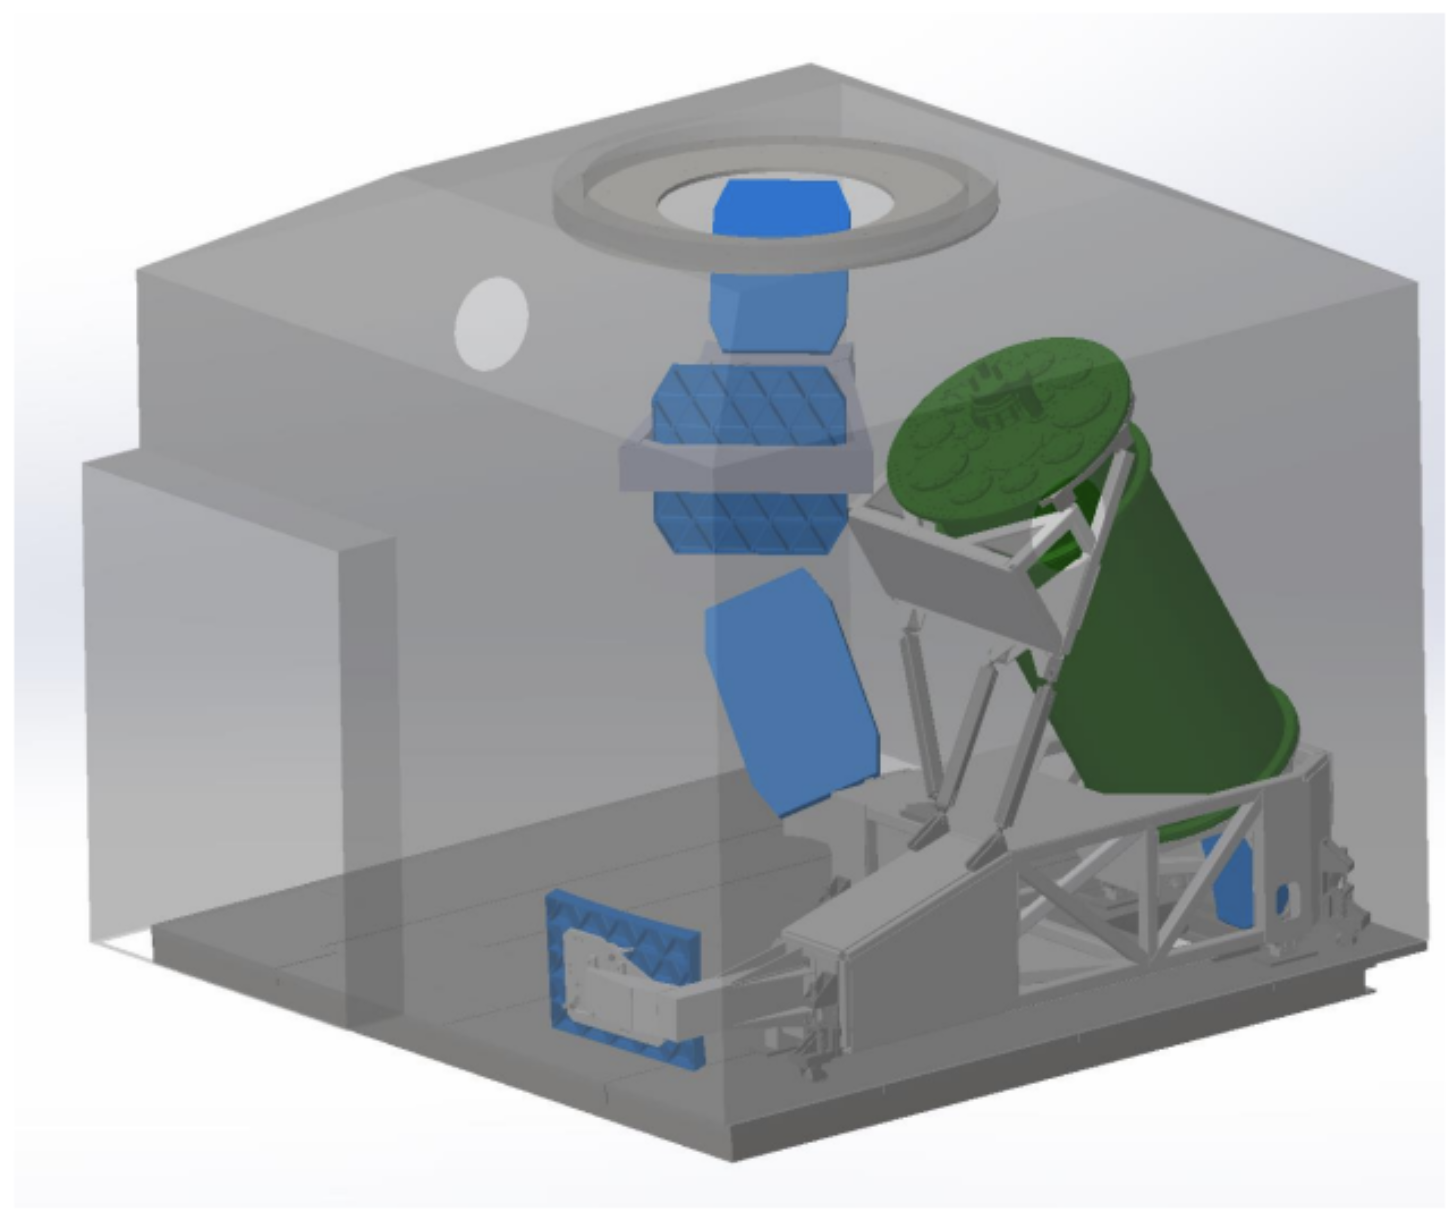
\includegraphics[width=0.45\textwidth]{cadoptpath.png}}}%
    \qquad
    \subfloat{{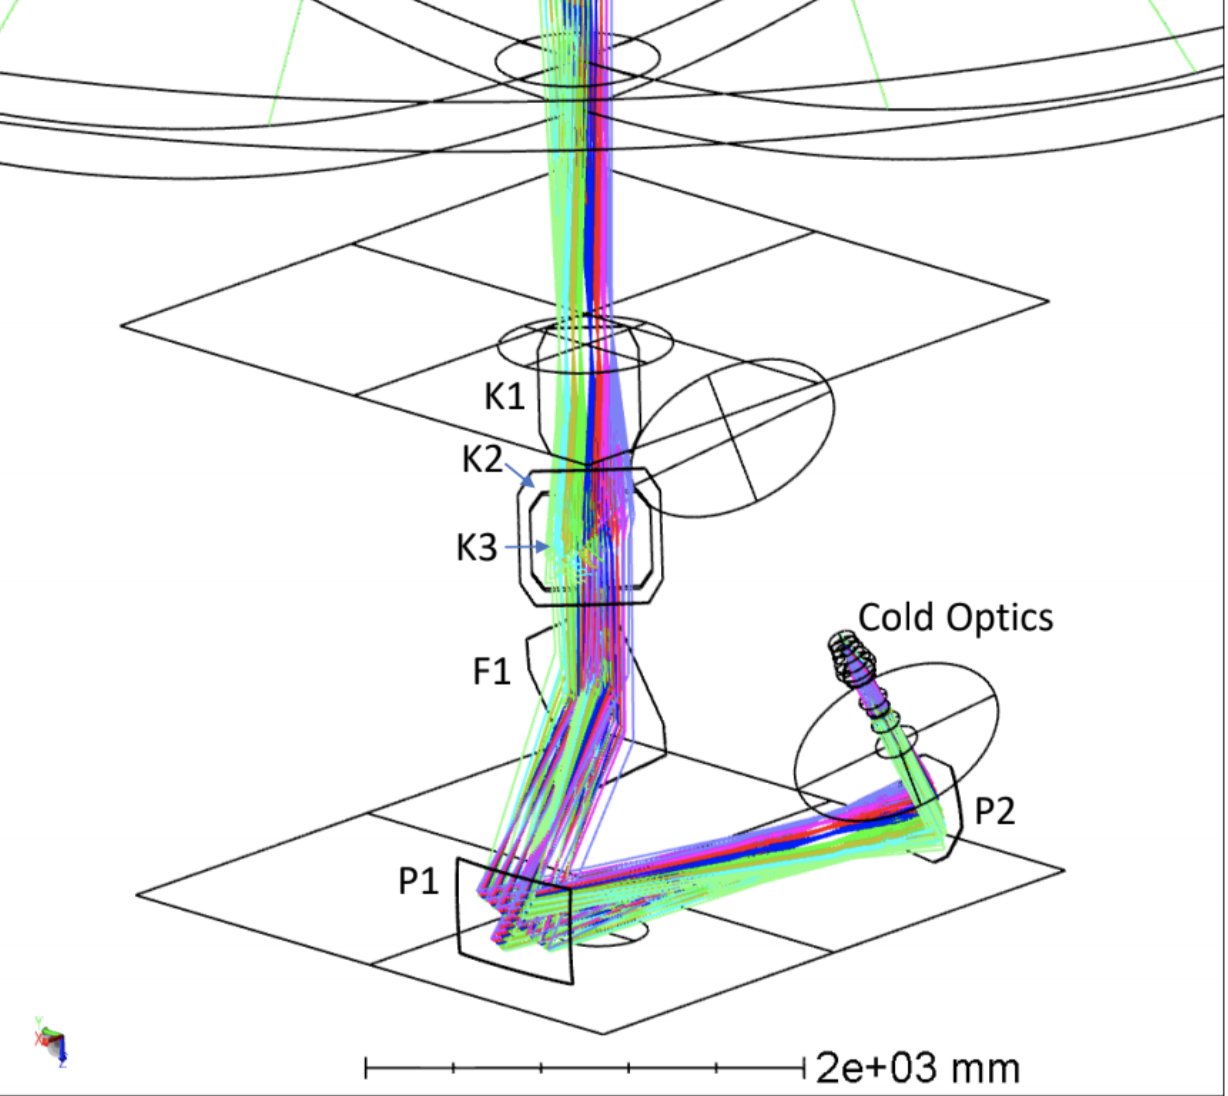
\includegraphics[width=0.45\textwidth]{optpath.png}}}%
    \singlespace
    \caption[TIME Full Optical Path in Telescope Cabin -(Isaac Trumper, UOA, TIME Collab)]{Left: CAD model of telescope cabin interior with optical components K-Mirror System and Cryostat. All blue objects are mirror interfaces. The green object is the cryostat that contains the cold optics. Right: Optical path {\sc Zemax} model of all three optical components, including three mirrors in the K-Mirror System, three focusing mirrors, and the cryostat cold optics. (Isaac Trumper, UOA, TIME Collab)}%
    \label{fig:optpath}%
    \vspace{-0.8cm}
\end{figure}

% \subsection{Telescope Optical Configuration}

% \begin{figure}[H]
% \centering
% \captionsetup{width=0.75\textwidth}
% 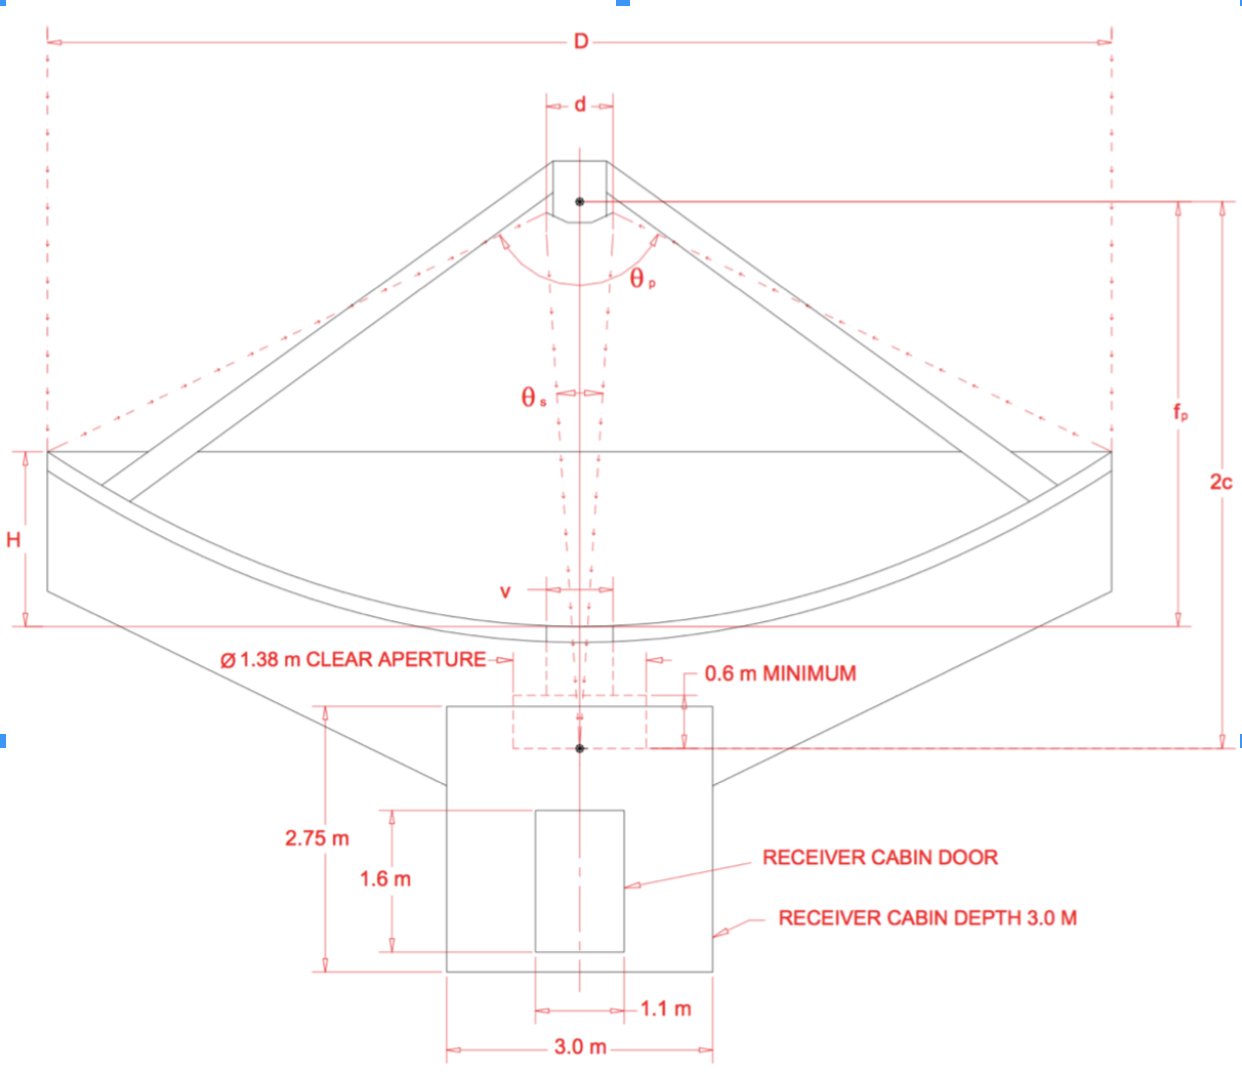
\includegraphics[width=0.75\textwidth]{telopt.png}
% \caption[ALMA Prototype 12m Optical Configuration -(Isaac Trumper, UOA, TIME COllab.)]{Scaled image of ALMA Prototype 12m Antenna Optical Configuration. Values for different scales are given below in Table~\ref{table:telopt} Other optical path elements are located inside the cabin of the telescope (Isaac Trumper, UOA, TIME Collab.).}
% \label{fig:tele}
% \end{figure}

% \begin{center}
% \begin{tabular}{|c|c|}
% \hline
% \multicolumn{2}{|c|}{ALMA Prototype 12m Telescope Optics}\\
% \hline
% \hline
% Primary Aperture (D) & 12.0 m \\
% Focal Length of Primary (\(f_{p}\)) & 4.8 m \\
% (\(f_{p}/D\)) of Primary & 0.40 \\
% Secondary Aperture (d) & 0.74 m \\
% Final f/D & 8.00 \\
% Magnification Factor & 20.0 \\
% Primary Angle of Illumination \(\theta_{p}\) & \(128.02^{\circ}\) \\
% Secondary Angel of Illumination \(\theta_{s}\) & \(7.16^{\circ}\) \\
% Distance Between Primary and Secondary Foci (2c) & 6.177 m \\
% Depth of Primary (H) & 1.875 m \\
% Primary Vertex Hole Clear Aperture (v) & 0.75 m \\

% \hline
% \end{tabular}\label{table:telopt}
% \end{center}

\subsection{K-Mirror Image Rotator}
The telescope at which TIME will be deployed rotates on an Alt-Azimuth mount, which presents unique challenges for the optical path from the primary mirror to the cryostat due to the line scan observation strategy (see section 5). The reason why can be seen in Figure ~\ref{fig:km1}, where the rotation of the earth causes objects on the sky to trace out a circular path with time. The telescope mount provides linear motion, meaning when the line of bolometers is projected onto the sky under this rotation, they show an unnatural overlap or gap when measuring the source with time.
\begin{wrapfigure}{r}{0.5\textwidth}
\vspace{-0.8cm}
  \begin{center}
    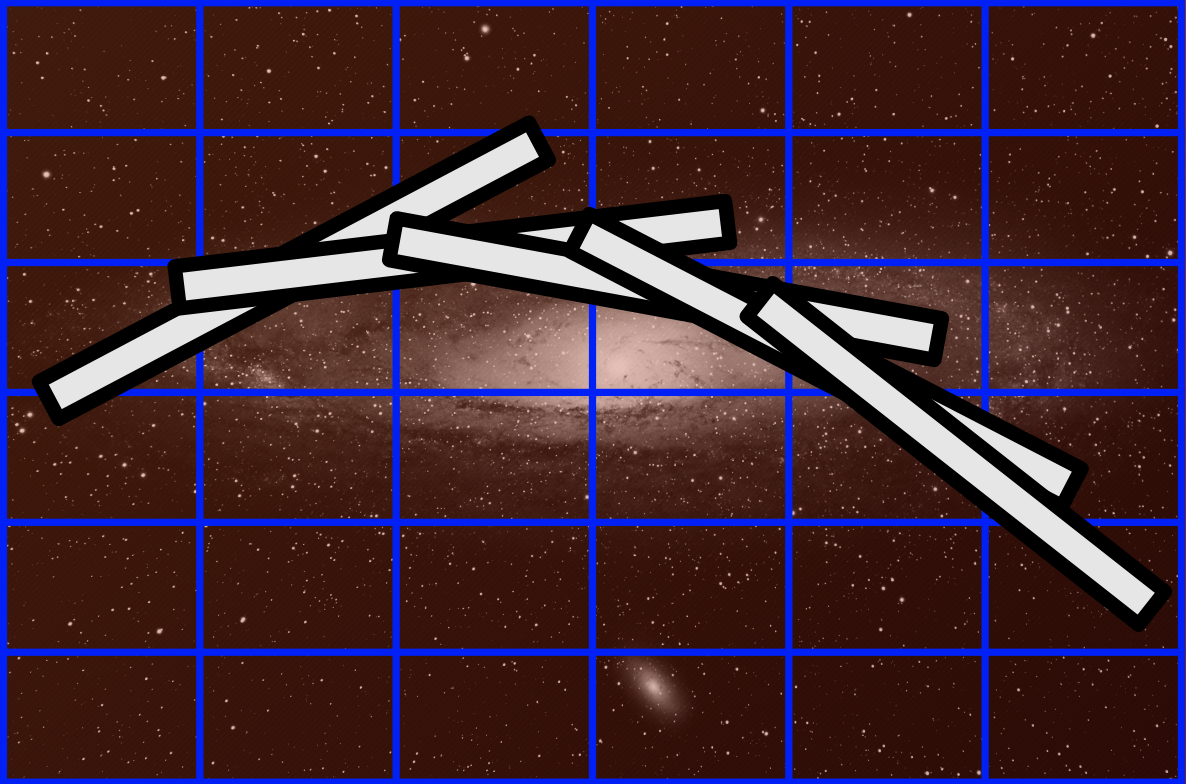
\includegraphics[width=0.48\textwidth]{km1.png}
  \end{center}
  \caption[Diagram of Bolometer De-rotation on Source from Alt-Az Mount.]{The white rectangles are a representation of the bolometer array projected on a galaxy source. As the galaxy naturally moves with time due to the earth's rotation, the line becomes rotated, causing overlapping regions and missing pixels. When the telescope moves to keep itself centered on the source, this problem would become more pronounced. For KSZ measurements, the resulting data would show extremely high thermal measurements in the centers of clusters, and almost none on the outskirts.}
  \label{fig:km1}
\end{wrapfigure}
The solution to this problem that will be implemented for TIME is to introduce an additional element into the optical path, which rotates the image plane before entering the cryostat, and becoming incident on the detectors. Figure~\ref{fig:km23} shows a CAD model of the basic structure for the K-Mirror System (KMS), consisting of two perpendicular mirrors to the rotation axis and one parallel.

The KMS is slaved to the motion of the telescope continuously, whether it is moving itself up to scanning position, tracking during an observation, or even in parked mode. Because of this, the telescope sends TCP/IP packets over an ethernet connection containing the current position and status flags directly to the KMS control computer ({\sc Raspberry Pi 3}). The motor and gearhead moving the system keep track of their position using an absolute encoder, which states the exact position attained by the system relative to the desired. After receiving the telescope data packets, an internal script in the Rasp Pi calculates the exact amount of rotation that is required to correct the image, based on the current position coordinates. This rotation is defined as half the parallactic angle.

\begin{figure}[H]
	\centering
	\subfloat{{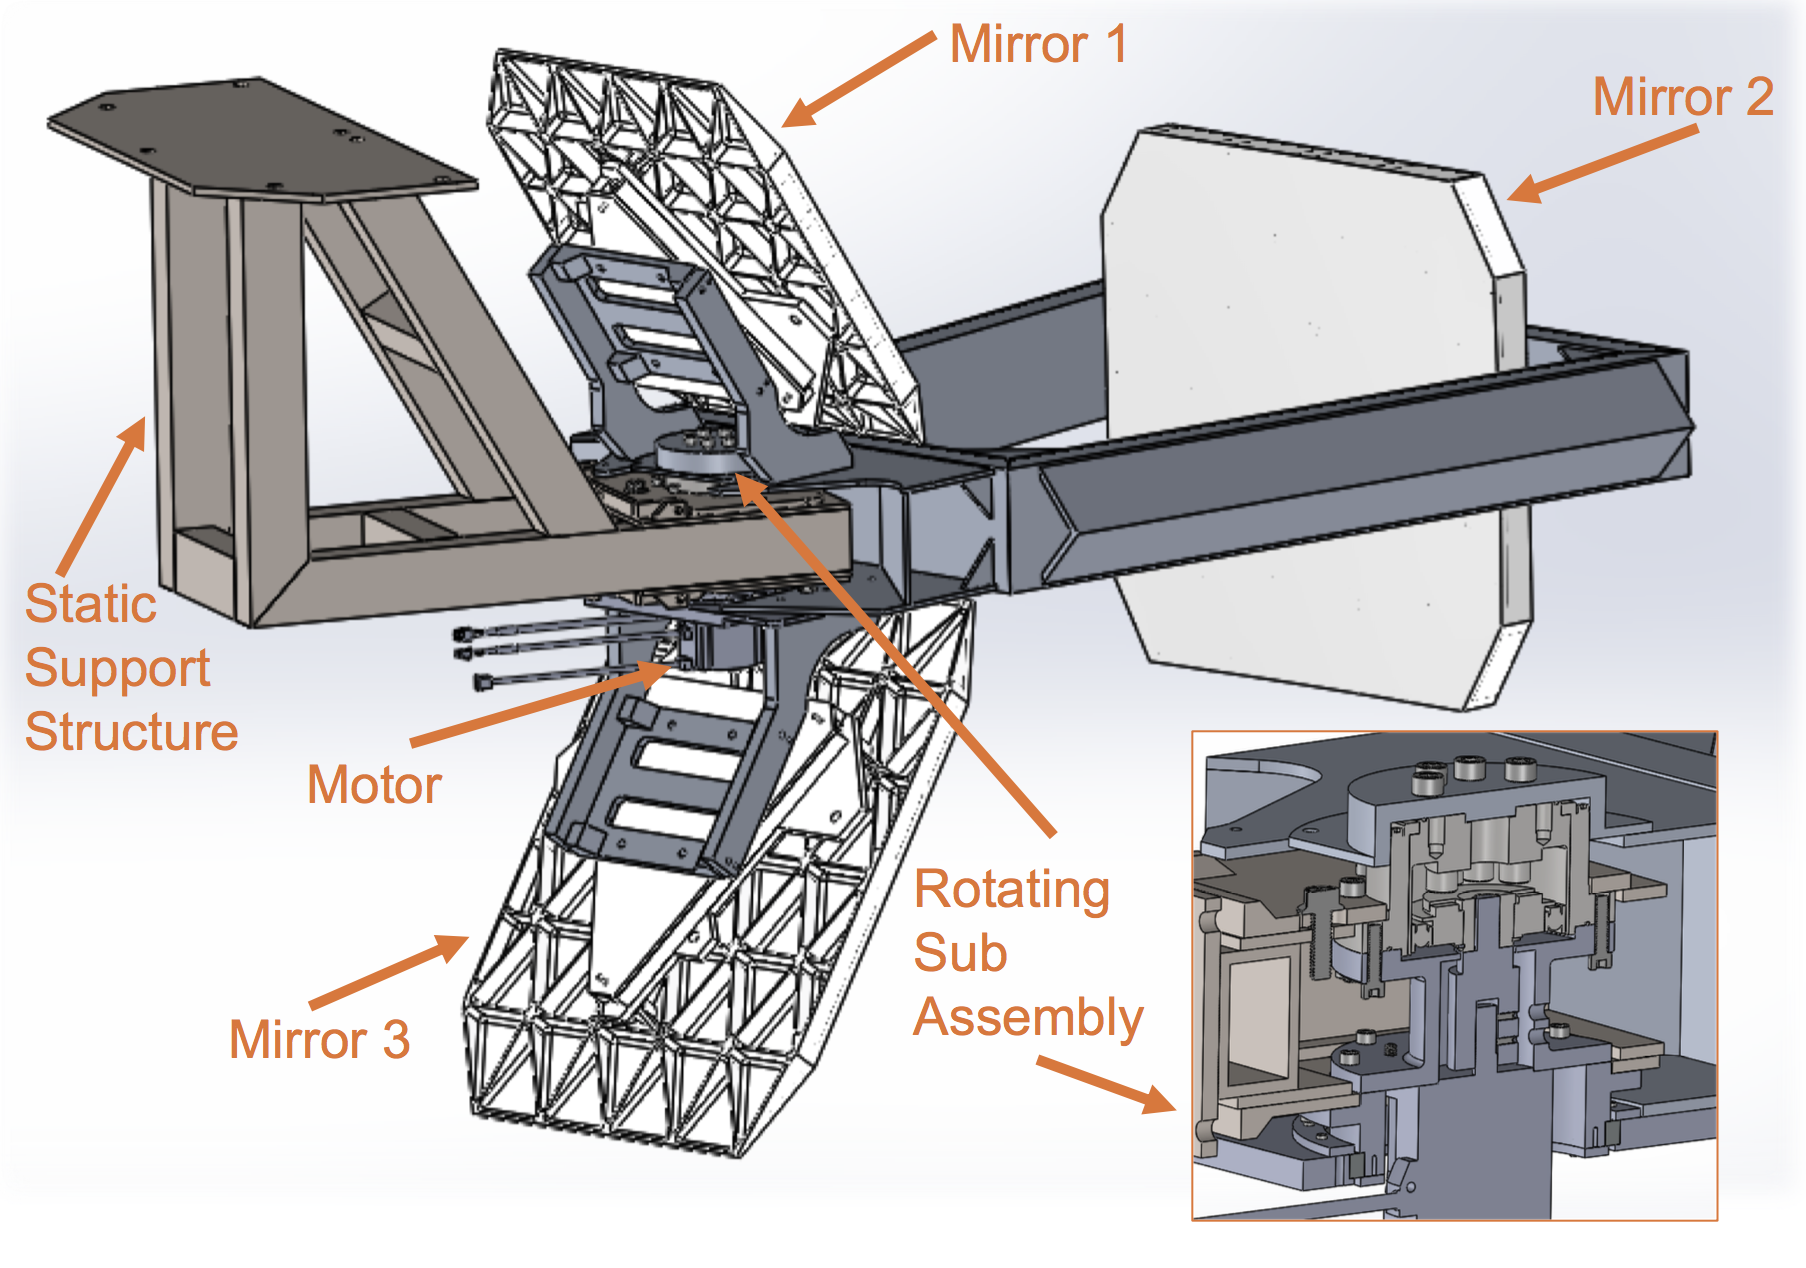
\includegraphics[width=0.45\textwidth]{km2.png} }}%
	\qquad
	\subfloat{{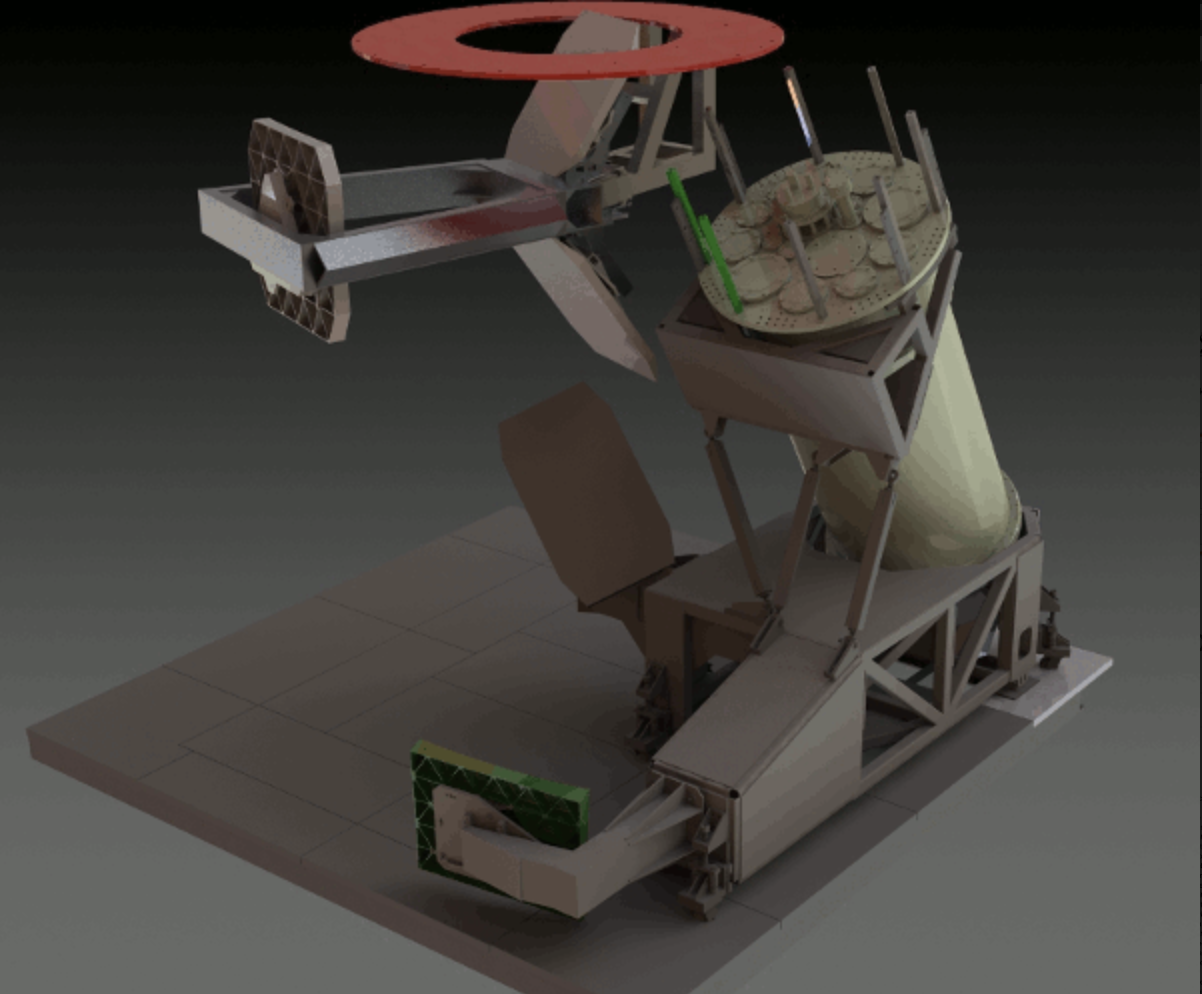
\includegraphics[width=0.45\textwidth]{km3.png} }}%
	\singlespace
	\caption[CAD Model of the K-Mirror Structure.]{Left: The K-Mirror structure consists of three main elements; the support structure made out of 80:20 aluminum, the mirrors, and the motor-gearhead-encoder rotation assembly. Right: The KMS is attached inside the telescope cabin to the flange (red circle) which is the optical input from the secondary mirror. Also shown is the TIME cryostat containing the instrument.}%
	\label{fig:km23}%
\end{figure}

The angle that describes the rotation in the cabin also defines the rotation of the observed source on the celestial sphere, where zero degrees of rotation is achieved when the object is at the local zenith. As the object travels before and behind zenith, the angle of rotation becomes more positive and more negative respectively. The equation which calculates this angle depends on the latitude of the observer, the hour angle (a function of the local sidereal time), and the declination of the object on the sky. The parallactic angle for an object is therefor completely unique for each observing site. Values for the KMS were calculated using position coordinates for Kitt Peak, where it will eventually be deployed. The equation is given below, which was taken from \cite{Meeus1998},
\begin{equation}\label{eq:parangle}
\tan(q) = \frac{\sin{(HA)}}{\tan(LAT)\cos{(DEC)} - \sin{(DEC)}\cos{(HA)}}
\end{equation}
where q is the parallactic angle, HA is the hour angle, LAT is the latitude, and DEC is the object declination. Some correctional factors are also calculated to increase the precision of (q), namely the true obliquity of the ecliptic and the nutation in longitude. Nutation in longitude accounts for the ``wobble" of the earth's axis caused by the moon, with some components having periodic fluctuations on the order of days. Obliquity of the ecliptic refers to the difference between the equator and the ecliptic, and how that distance is variable with time.

Some uniques software challenges exist for the KMS in the event that it travels through zenith, since Equation~\ref{eq:parangle} generates and undefined solution.  
\begin{wrapfigure}{r}{0.5\textwidth}
\vspace{-0.8cm}
  \begin{center}
    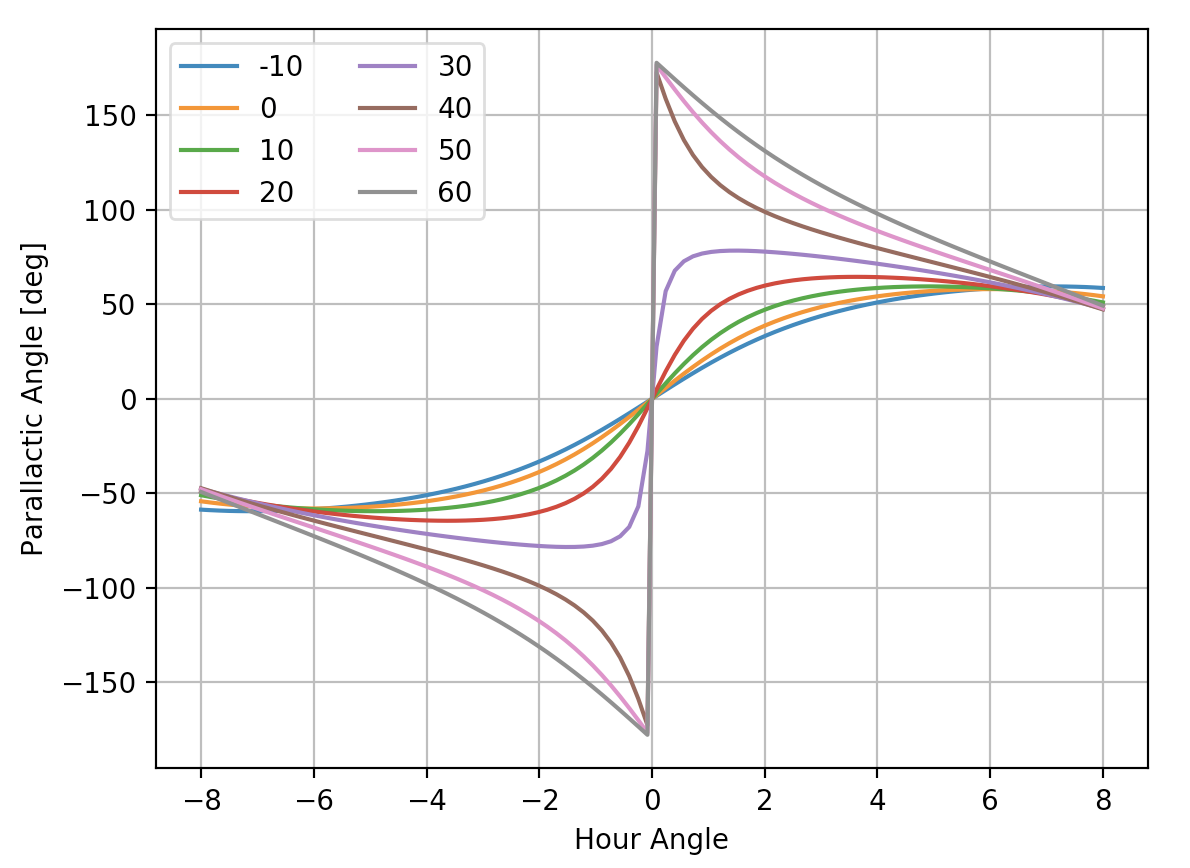
\includegraphics[width=0.55\textwidth]{km6.png}
  \end{center}
  \caption[Parallactic Angle Versus Hour Angle]{The KMS will hit wraps at the observers local zenith. This graph of PA vs. HA shows that this location is roughly +7 and -7 around 0 HA. The speed at which the KMS would move towards zenith depends on the telescopes declination. The values in the legend correspond to different lines of constant declination on the graph, in degrees.}
  \label{fig:km6}
\end{wrapfigure}
The movement of the KMS at this location would be a rapid jump from $- 90^{\circ}$ to $+ 90^{\circ}$, which is not mechanically feasible. The total weight of the system combined with the torque limits of the motor would make a huge jump impossible for the KMS to achieve in a reasonable amount of time, and would result in motor failure. 

Solutions to this problem are three-fold, one set of checks is put in software, another in hardware, and the last is mapping which observing regions contain these problem areas. The easiest is hardware, which involves adding a hard stop limiter that will be tripped if the KMS attempts to move outside of a safe set of ranges. If one of these limit switches is tripped, an error flag will be sent to the command computer, and the system will be stopped. This is meant to be a last resort. In software, a system of checks is implemented to prevent over rotation, and rapid rotation.

The most efficient way of avoiding problems near zenith is to determine positions and times objects in the sky at Kitt Peak will pass through the local meridian. Two different visualizations were made to assist in determining these problem areas. Figure ~\ref{fig:km6} revealed that for a starting observation of local midnight, the KMS could only observe continuously for roughly 6 hours before it would reach local zenith. The left graph of Figure ~\ref{fig:km45} shows for the same period of time, at what coordinates on the sky those zenith positions are located. The right graph is a comparison for the physical location of the second mirror arm in the cabin at zenith. Any location near the cryostat, or next to the left hand wall will also require a wrap of the arm, in addition to the zenith positions. Any position below 25 degrees in declination appeared to be safe at all times of the night. Because of these limitations, the KMS plays an integral role in the determination of an optimal observation strategy.   

\begin{figure}[ht!]
	\centering
	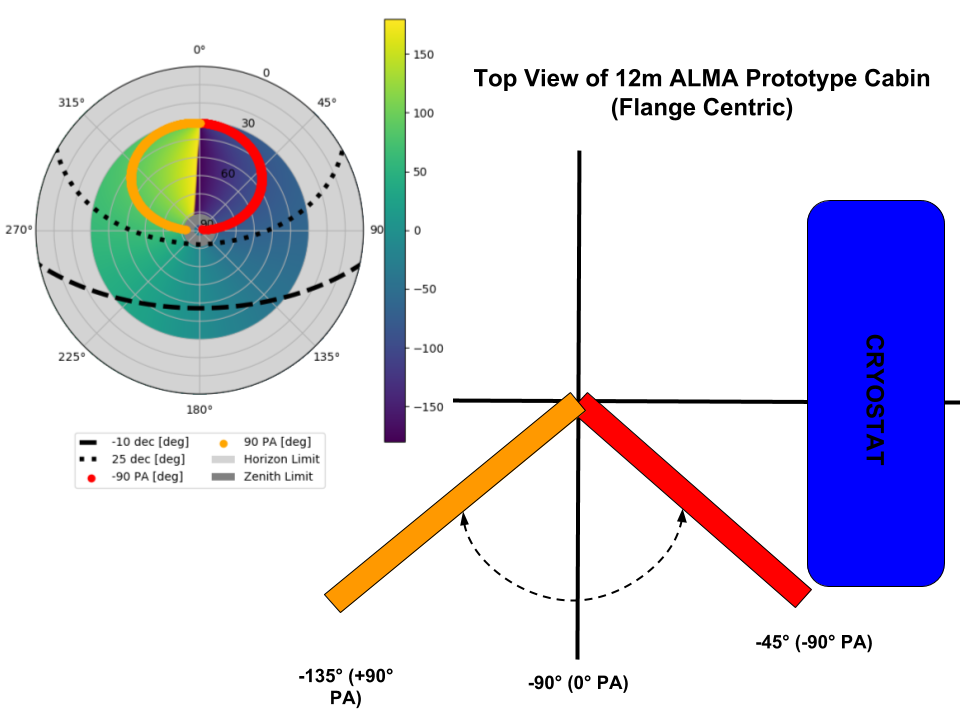
\includegraphics[width=\textwidth]{km45.png}%
	\caption[Parallactic Angle Graphs to Determine Zenith Positions]{Left: Polar graph of all declinations and right ascensions as viewable at Kitt Peak. The parallactic angle is the color scale given in degrees. This plot are the PA's for the sky at midnight. Any region on the sky, as viewed from the telescope, that reaches $-90^{\circ}$ or $+90^{\circ}$ PA would require a wrap of the K-Mirror arm back through $0^{\circ}$ PA, which would involve a minimum $45^{\circ}$ rotation. The dotted and dashed lines correspond to 25 deg dec and -10 deg dec respectively. The region shaded in gray represents a region that is unobservable by the telescope. Right: Top down view of the KMS, with the cryostat added for reference. The colors of the arms correspond to the lines of the same color on the plot.}%
	\label{fig:km45}%
\end{figure}

\newpage
\section{Observation Strategy}

TIME is utilizing grating spectrometers that are capable of rendering not only spectral but also spatial information into a 3 dimensional data cube. This adds the benefit of separating a superposition of signals from different redshifts along the line of sight, but in the same spatial pixel. For research on the CMB and the EOR, this is an especially useful tool as it allows both foreground and background sources to be individually measured. In the case of TIME, this implies the ability to distinguish between the faint dwarf galaxy population of interest and the much brighter foreground galaxies. 

Complementary to the spectrometers, the chosen observing method will have the ability to constrain faint CO and CII line emission at high redshift though intensity mapping. This is a tested technique [\cite{Keating2015},\cite{Keating2016}] accomplished by moving the array of detectors across the sky, and recording the spatial variation in the total surface brightness from all sources in the field of view (FOV), as bolometer arrays are sensitive to the integrated intensity. Traditional measurements of faint galaxies attempt to resolve a single source through interferometry, such as with the Atacama Large Millimeter Array (ALMA), but typically miss the faintest end of the full luminosity function. With intensity mapping, lower limits on the faint end of the function can be determined, using only a single dish, rather than an entire array. Compared to ALMA, which would take roughly 4500 hours to observe a 2.5 degree FOV [\cite{Kovetz2017}], TIME can scan that same area in 1000 hours. The survey parameters for different sources is given in the table below. 

\begin{center}
    \begin{tabular}{|c|c|}
    \hline
     \multicolumn{2}{|c|}{TIME Survey Parameters} \\
     \hline
     \hline
      Atmospheric PWV Monitor Channels & & 10: 183-199 GHz & 6: 305-326 GHz \\
      Instantaneous FOV (ARO 12m) & 14 arcmin x 0.43 arcmin (mid-band) \\
      CII Survey Volume & 153 Mpc x 1.1 Mpc x 1240 Mpc deep \\
      CII Survey Integration Time & 1000 hours \\
      kSZ Peculiar Velocity Sensitivity & $\pm 1000 km/s$ per beam in 10 hours \\
      \hline
    \end{tabular}
\end{center}

TIME will be commissioned at the Arizona Radio Observatory (ARO) at Kitt Peak on the 12 meter ALMA Prototype Antenna in February 2019. Once there it will undergo a series of tests and calibrations, and will eventually start observations. It will be completing constant declination scans of several individual clusters by rastering back and forth across a source. An example scan pattern is shown in Figure~\ref{fig:time2ab}  and~\ref{fig:time2cd} below. The ideal strategy will be to scan two 1.3 degree linear fields over the course of 9 hours for CII/CO, and further dedicated time for kSZ detection in selected galaxy clusters.

\begin{figure}[H]%
    \centering
    \subfloat{{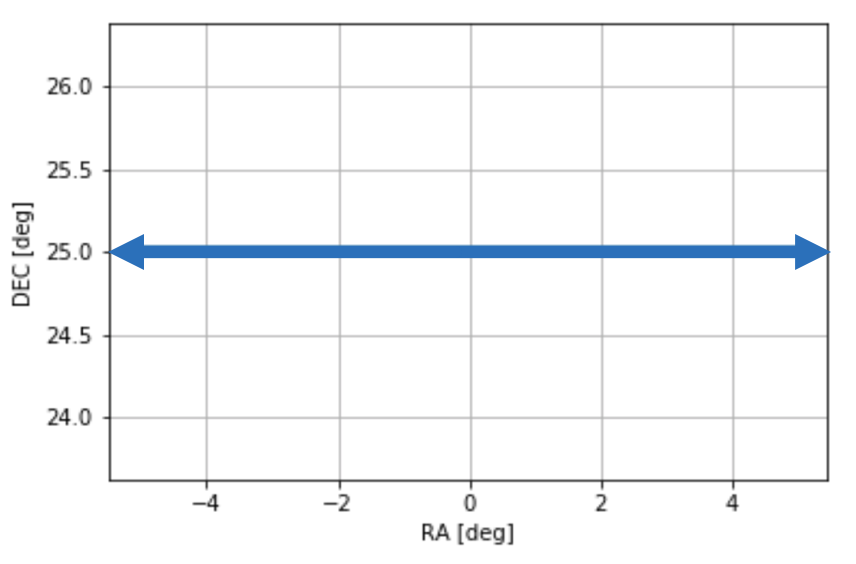
\includegraphics[width=0.45\textwidth]{time2a.png} }}%
    \qquad
    \subfloat{{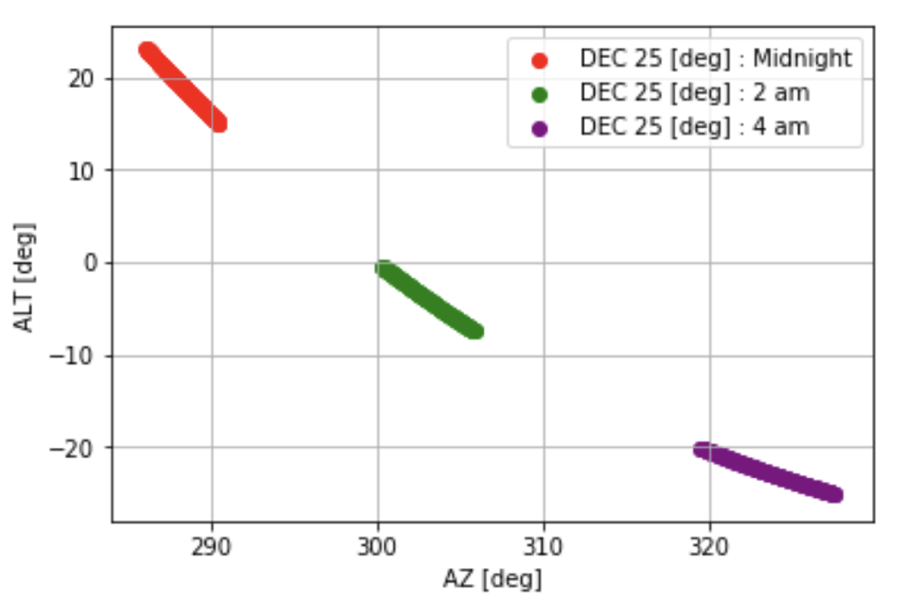
\includegraphics[width=0.45\textwidth]{time2b.png} }}%
    \singlespace
    \caption[TIME Scan Strategy 1]{Left: Arrows indicating motion back and forth across an exaggerated 10 degree field of view, constant in declination. Right: Same scan pattern but given in ALT-AZ coordinates, with different colors showing start of observation at different times for Kitt Peak.}%
    \label{fig:time2ab}%
\end{figure}

\begin{figure}[H]%
    \centering
    \subfloat{{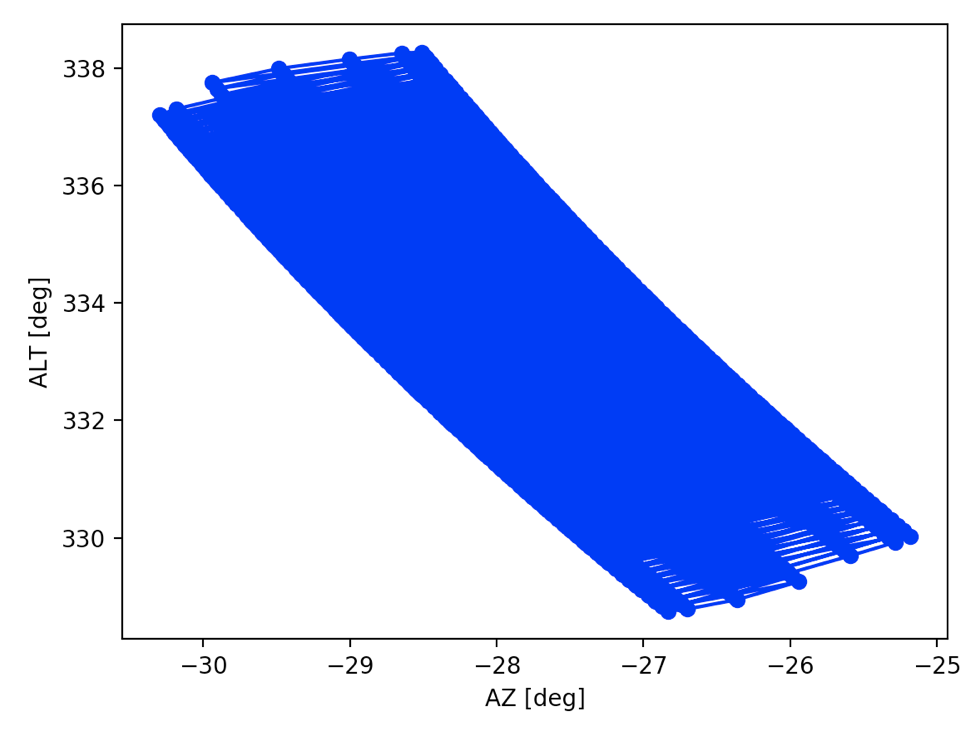
\includegraphics[width=0.45\textwidth]{time2c.png} }}%
    \qquad
    \subfloat{{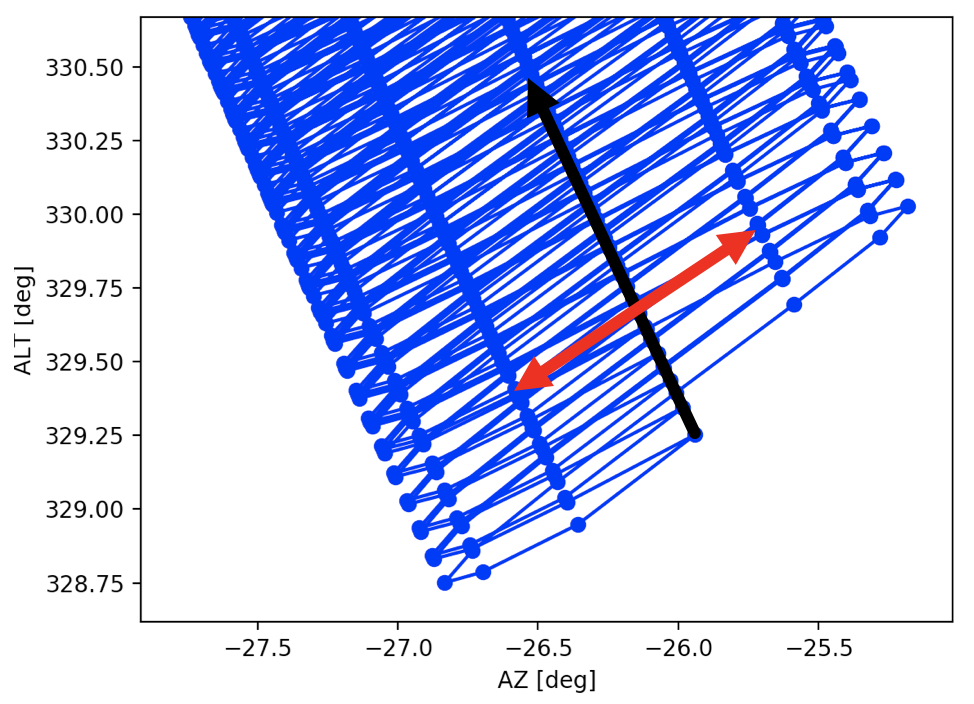
\includegraphics[width=0.45\textwidth]{time2d.png} }}%
    \singlespace
    \caption[TIME Scan Strategy 2]{Left: Closeup of one time of observation in ALT-AZ coordinates, showing how the rastering across the source appears to make a helical motion, due in part to objects moving across the sky while observing. Right: Increased zoom of the left figure. Red arrow shows the motion back and forth across a line of constant declination, while the black line indicates the observed sources path across the sky.}%
    \label{fig:time2cd}%
\end{figure}

\newpage
\section{Data Collation, Visualization, Storage \& Analysis}

\subsection{Graphical User Interface}
For lab testing and on-site live data visualization, a graphical user interface (GUI) was designed in a {\sc Python} script, and initially implemented in a web based framework using {\sc Dash by Plotly}. The GUI acts like a HUB, with input and output to multiple devices which all show statuses on the screen. Currently added functions include viewing the data from the MCE, with both live and archival data, a heatmap of the detector channels, and simulated inputs from the K-mirror and telescope. Figures ~\ref{fig:gui1} and ~\ref{fig:gui2} show the first and second iterations of the GUI. In the first iteration, the MCE was activated by a python script, the incoming data was parsed by another script and fed to the Plotly servers, and then a separate script stored the data in a preferred format. A web browser could then be opened and sent to a local host address where the user could view and interact with the data. This version was abandoned after testing the MCE at the highest data rate of 400 Hz, with 2 seconds of data on the screen at a time, updates every 1 second, and run for 8 hours. At this data rate, the MCE generates 374 frames per second. When looking at the output for only one detector, 374 data points are added to the screen per second, with over 12,000 data points present in every array. When run for an extended time, the lag on screen became visibly noticeable, as it would take longer and longer for the graphs to update, and some frames were even skipped entirely. This was due to the method by which Plotly updated its streaming plots, where it would have to re-draw every data point every time the graphs were refreshed, meaning that after 30 seconds, 11,000 data points were on the screen at a time. For lab testing, it was necessary to have at least 2 minutes of data on the screen at one time.

\begin{figure}[H]
	\centering
	\captionsetup{width=0.85\textwidth}
	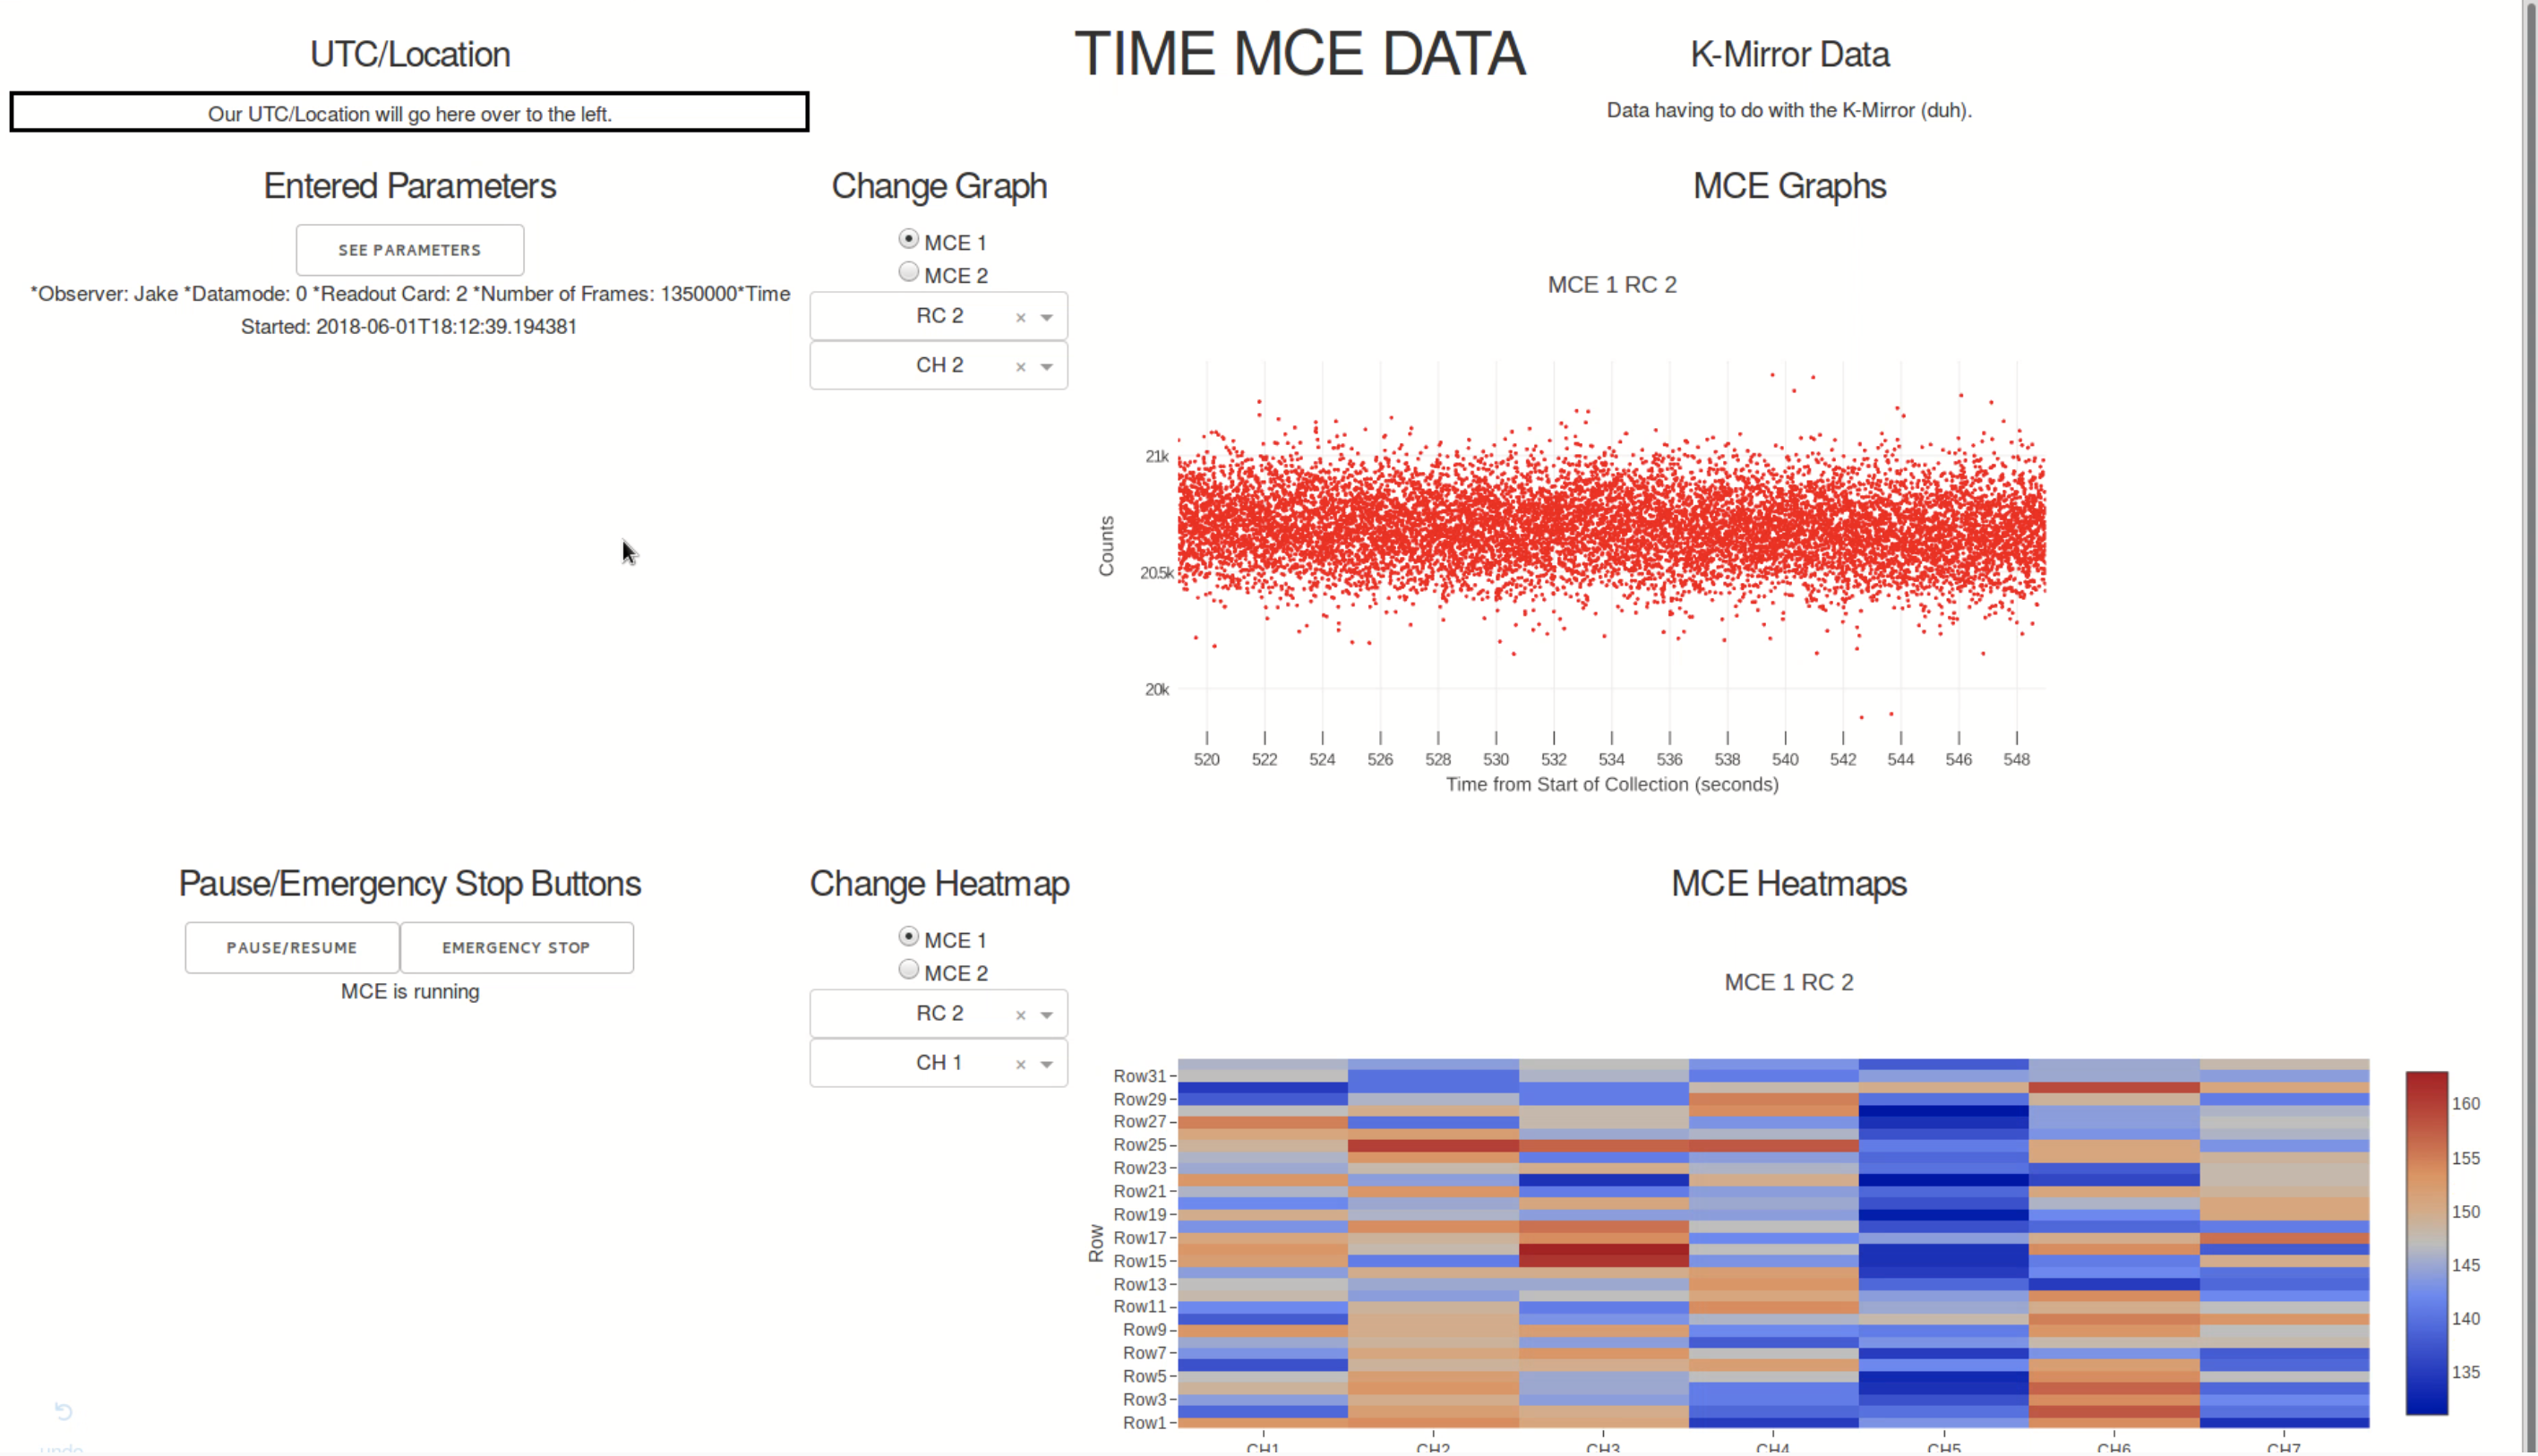
\includegraphics[width=0.85\textwidth]{gui1.png}%
	\caption[GUI Beta 1.0]{This GUI was made through the use of {\sc Dash by Plotly} which handled all data updating and viewing on the screen, as well as activating the MCE and providing an interactive user interface. This version was abandoned for the unreliability of web servers, and severe lag after several minutes.}%
	\label{fig:gui1}%
\end{figure}

\begin{figure}[H]
	\centering
	\captionsetup{width=0.85\textwidth}
	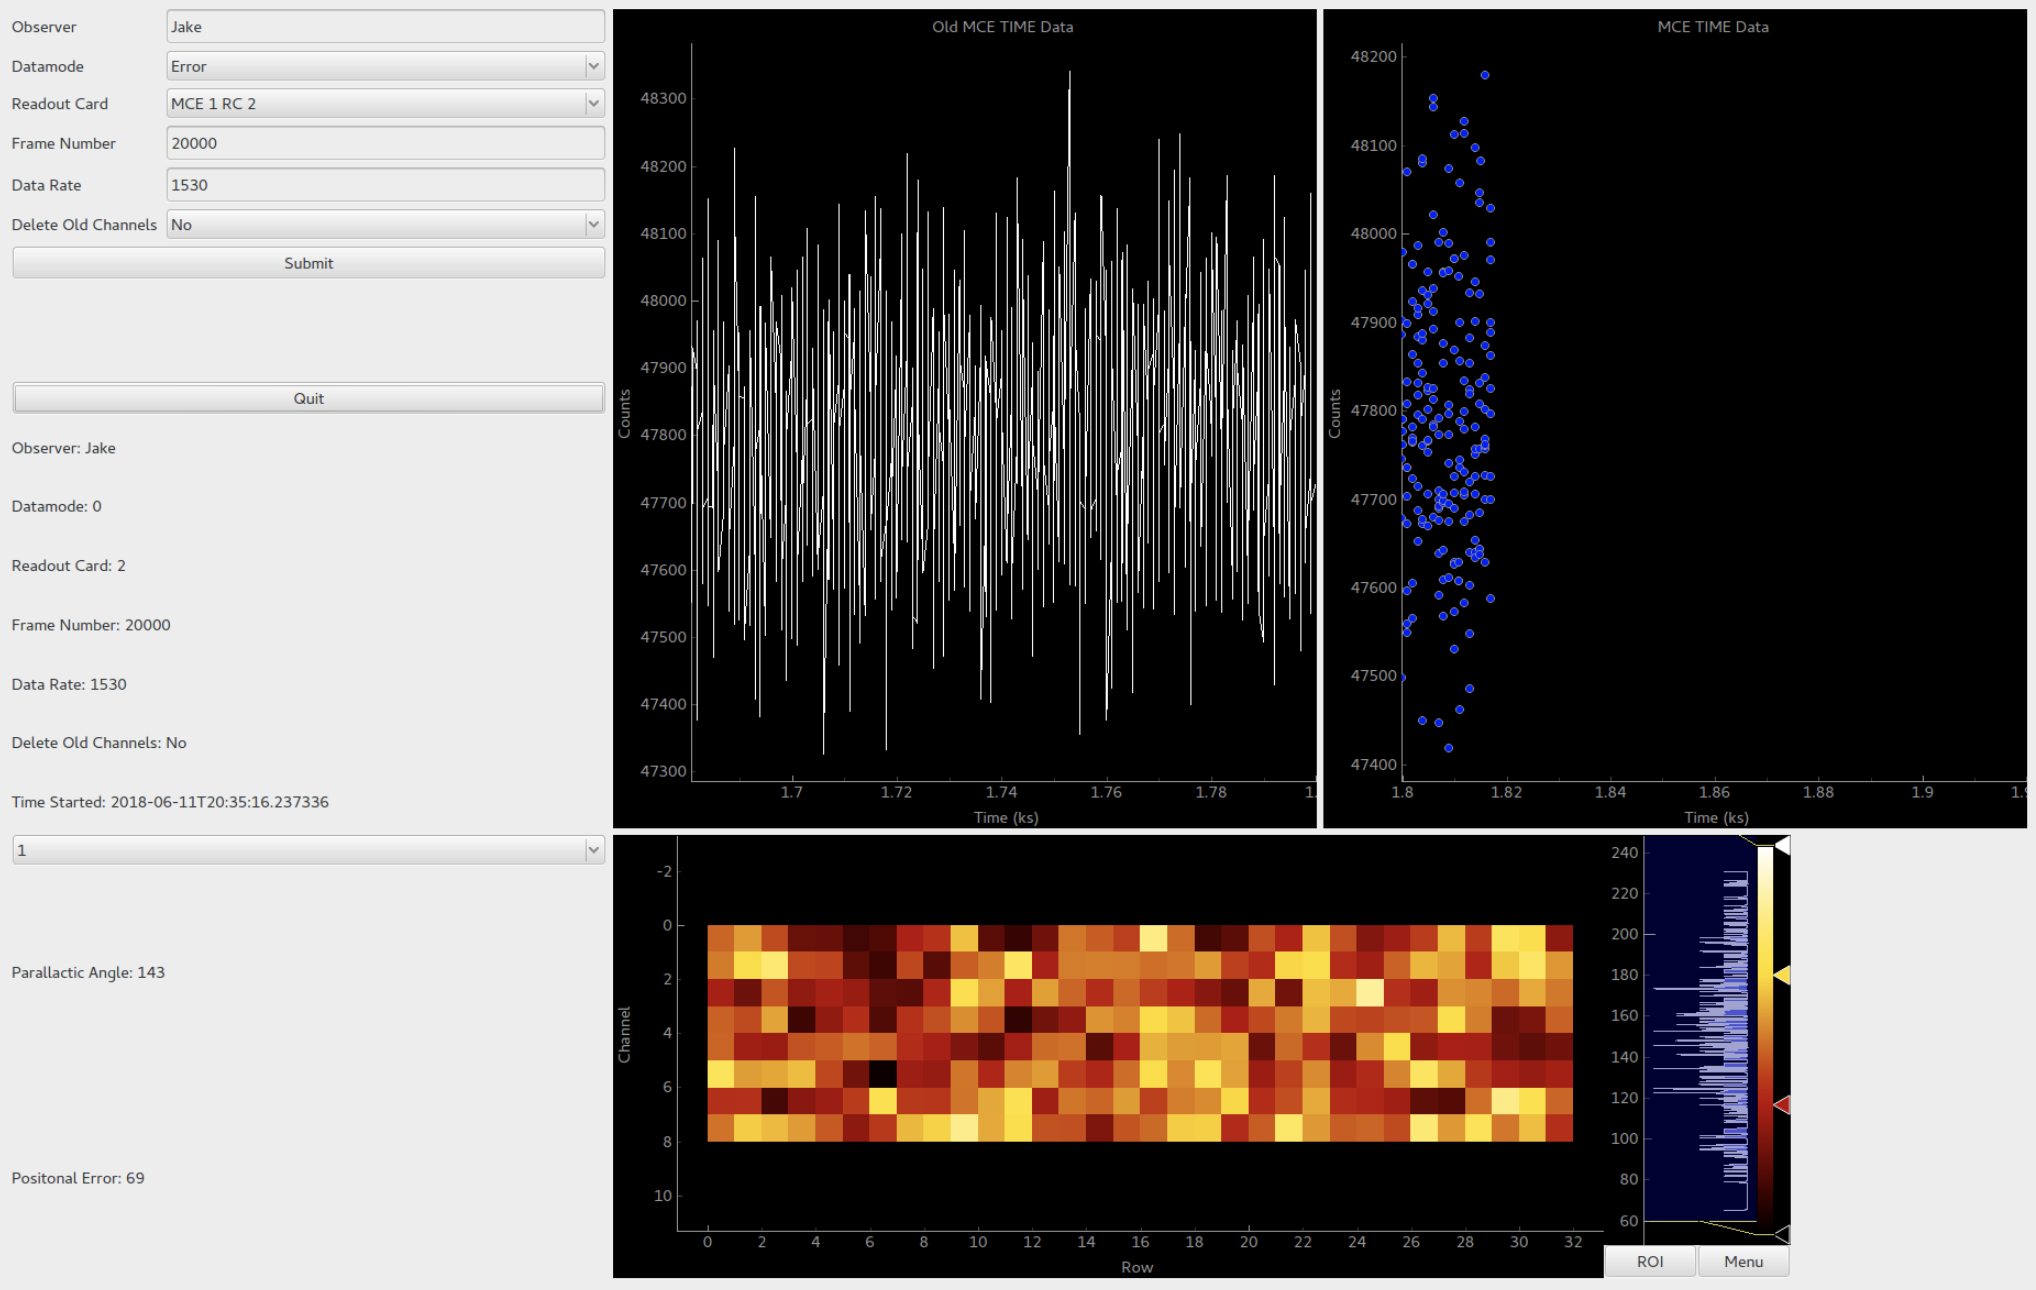
\includegraphics[width=0.85\textwidth]{gui2.png}%
	\caption[GUI Beta 2.0]{Version 2 of the GUI was done using a desktop interface created with {\sc PyQTGraph}. This gui had the advantage of using much less CPU, almost no lag after continuous running, and more versatility for customization.}%
	\label{fig:gui2}%
\end{figure}

The second version of the GUI was created using PyQt4 graphics packages and required a re-write from the html based script employed before. This script only updated the graphs with the newest data, without redrawing the whole figure, and wasn't subject to the unpredictability of web servers. The necessary packages could also simply be downloaded through ``apt-get'' from a standard library and added to the users existing python library. This new system was tested using the same parameters as the first, which revealed only one minor flaw. The parameters for the MCE input by the user, including data rate, would return a frame per second that would not be an integer value. At a data rate of 45, the value was exactly 374 frames per second, but at a data rate of 10, it was 1683.5 frames per second. This meant that every other second, an extra file was created, and missed by the previous check by the software. This was easily corrected for by adding in a check for an extra file that would be parsed and incorporated onscreen in the correct chronological order. After testing the system with 5 minutes of data onscreen at a time for 8 hours, there were no lags to the system. 

Items that must still be incorporated into the GUI are actual interfacing from the K-Mirror and the Telescope. A telescope simulator was created to mimic the observing patterns required for TIME (constant declination scans) which outputs positional information and other metrics necessary for the K-Mirror operation described in detail later. The next step in testing will involve data generation from these simulated sources, transferred over SSH, and then visualized on the remote observing computer. 


\subsubsection{KMS Integration \& Testing}

Two different tests have been run on the software, one which tested exclusively the ability to manipulate the given data and produce corrections in rotation and speed, and the other with a more realistic simulation and use with the motor and encoder. The first test was run with a simulation which mimicked the telescope moving back and forth in a straight line. The top left of Figure ~\ref{fig:km78} shows the absolute position as reported by the simulated telescope, with a change in direction clearly shown halfway through. The error graph shows an average offset of the KMS from the desired position of 14 arcseconds, with a maximum error of 100 arcseconds. The third plot is the reported motor speed, and the last graph is the software attempting to compensate for varying speeds of data packets and updates from the telescope. There are two different types of errors being corrected for here. One is the inability of the KMS to correct for differences in the actual versus desired rotational position, and the other is caused by the variability of the telescope data. In the telescope data transfer is some intrinsic noise caused by the data packets arriving at variable speeds, the updates each having a different values, the imperfect speed of the telescope, and the variable response of the KMS. For example, there are certain circumstances where the telescope may send updates at a rate of 40 packets per second, and have such a slow speed that an update to the position of the KMS is not required at each update, and then an update in position is required at the 29th packet. The transition from stationary to moving is jarring for both the software and mechanical system. 

\begin{figure}[H]
	\centering
	\captionsetup{width=\textwidth}
	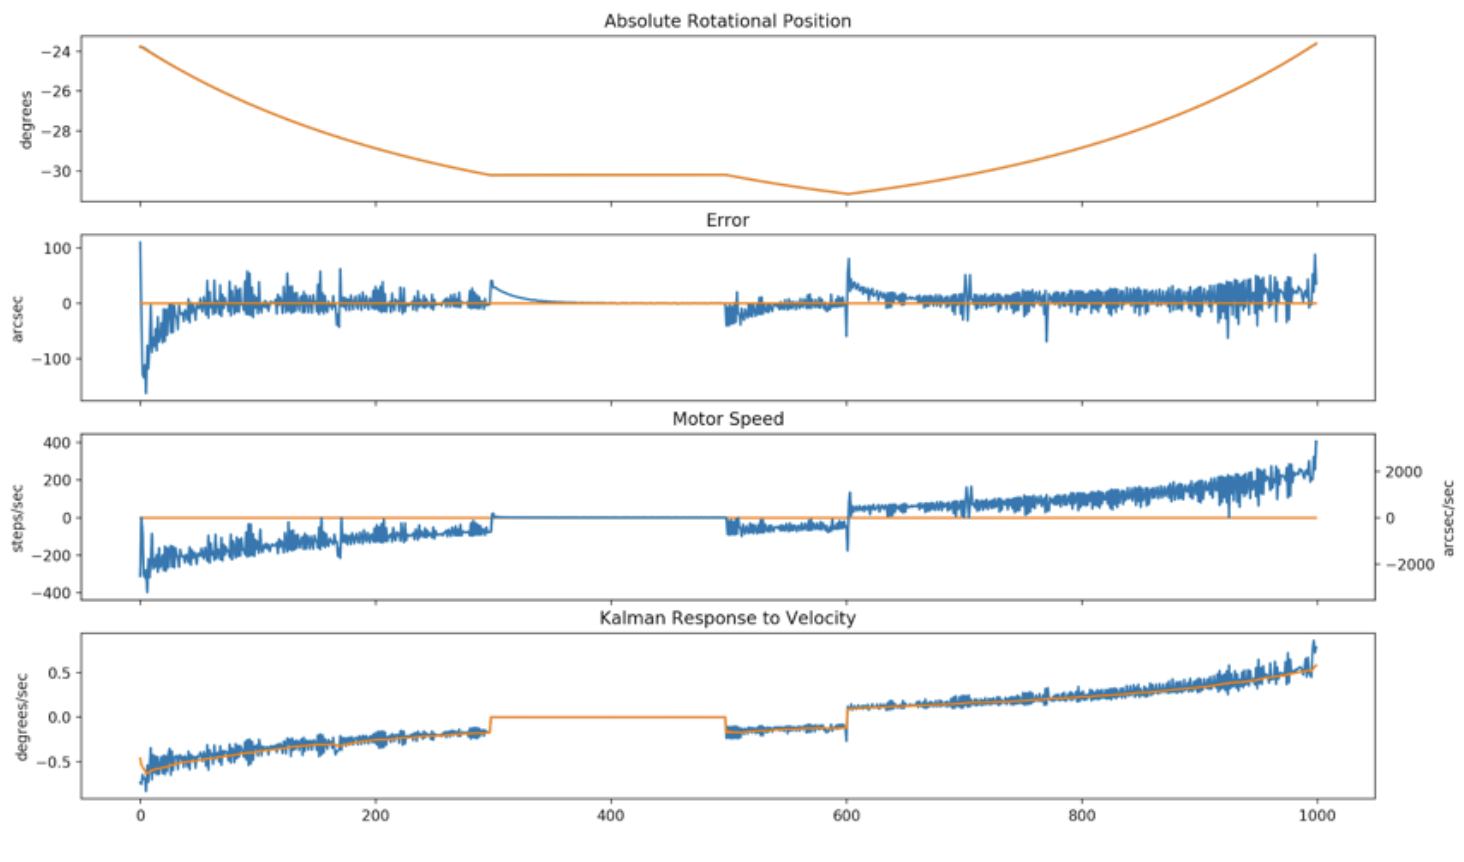
\includegraphics[width=\textwidth]{km7.png}%
	\caption[Simulated KMS Performance, Simple Rastering Scan]{Simulation showing the KMS software response to telescope input at sidereal rate, 20 packets per second data rate, moving back and forth across the same declination. Orange is the information passed from the telescope, and blue is the response by the KMS. From top to bottom it shows the absolute rotational position as given by the telescope, the error between the telescope position and the resulting position of the KMS, the KMS motor speed, and the Kalman Filter changes with a change in velocity from the telescope.}%
	\label{fig:km7}%
\end{figure}

\newpage
\begin{figure}[H]
	\centering
	\captionsetup{width=\textwidth}
	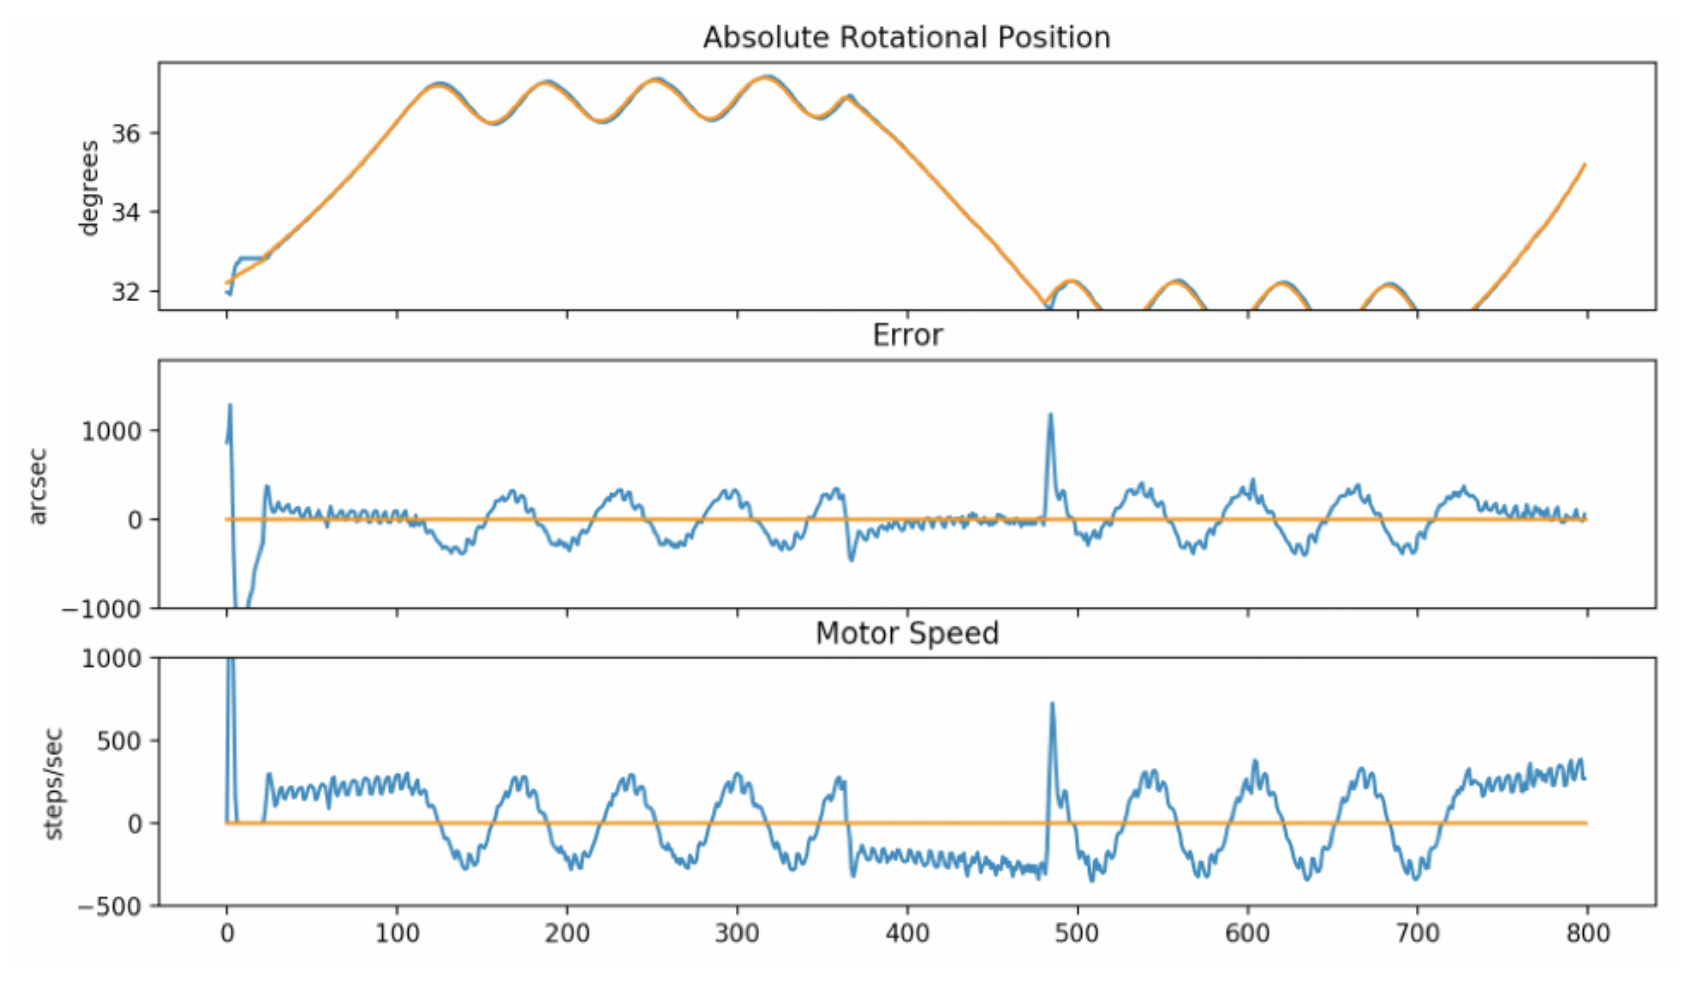
\includegraphics[width=\textwidth]{km8.png}%
	\caption[Simulated KMS Performance, Realistic Box Scan]{Simulation showing the KMS motor, encoder and software response from telescope input at 5'' - $1^{\circ}/s$, 20 packets per second data rate, making a sinusoidal (or imperfect box) scan. Orange is the telescope position, and blue is the KMS response. The graphs have the same meaning as those above. The only difference is that the relative error is much higher for this case, due to the change in velocity around the peaks and troughs of the sinusoid, and the change from slewing to a position (straight line) versus tracking a source (sinusoid).}%
	\label{fig:km8}%
\end{figure}

To address this, a Kalman Filter [CITE REFERENCE HERE] was applied to interpret the telescope data based on data rate, relative velocity changes, and the total change in position required. This algorithm creates an unbiased estimate of the natural ``noise'' of the telescope-K-Mirror system, and then continually corrects the data for this average error, and updates this average error over a period of time. This allowed the motor to more smoothly start and stop, and improved the ability of the software to correct for changes in observational modes. Figure ~\ref{fig:km8} shows this improvement on the actual motor, gearhead and encoder with a more sophisticated telescope simulator. In the first simulation, the telescope speed was set to the sidereal rate, with a box-like pattern of motion set of coordinates provided to the KMS. The second simulation included a ``slewing'' phase, where the telescope was moving at 1 degree per second up to a starting position, and then a ``tracking'' phase at 5 arcseconds per second, where the telescope was moving back and forth across the given coordinates. This scenario produced a line scan akin to TIME, and at roughly the correct observing speeds. This test proved that the software and motor were capable of keeping up with the telescope even at its fastest speed while also reducing error to within tolerances.  Additional testing includes adding the mirror mass models and using the software and motor under a load bearing case, and simulating data transfer from telescope to KMS over an isolated network server. A script designed to simulate telescope socket data transfer has already been written by the University of Arizona and has been successfully integration into the GUI software. 

The KMS software was designed to integrate with the GUI in order to facilitate real-time monitoring of its status. It receives input directly from the telescope, but only sends output to the control computer. This includes several flags for emergencies, like ``emergency stop'', ``standby'', and ``rotating''. There is no way for the control computer to directly communicate with the KMS, and instead will be done by way of the telescope. This reduces the complexity of code necessary for controlling the KMS, reduces the load on the Raspberry Pi 3, and creates less opportunity for software malfunction. In a situation where there is a problem with the KMS, MCE, detectors, or any other connected component to the control computer, an emergency stop button can be pressed on the GUI, which will send a signal to simultaneously stop all other processes (i.e. telescope motion, data acquisition, etc.) Additionally, the current parallactic angle will be output on the screen next to the angle achieved by the KMS, as well as the current speed.

\subsubsection{TIME Software Development}

In order to facilitate the successful completion of the TIME scientific goals, an important consideration is the handling of data and intercommunication between devices.A schematic of the hardware layout and connections is included in Figure ~\ref{fig:km9}, which details the communication pathways for multiple devices, including the telescope, control computer, Multi Channel Electronics (MCE), K-Mirror, and others. The key to successful data acquisition will be synchronous operation of each system, and eventual data collation. 

\begin{figure}[H]
\centering
\captionsetup{width=0.95\textwidth}
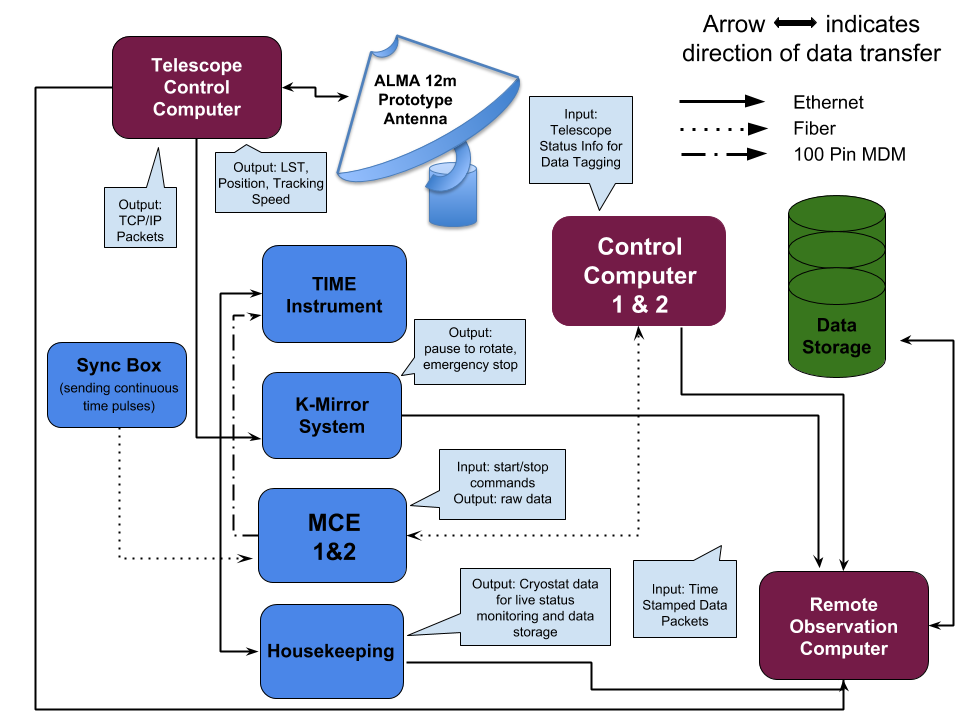
\includegraphics[width=0.95\textwidth]{km9.png}
\caption[TIME Control Flow Diagram]{Communications layout for TIME. Each instrument in blue represents a source of data, some of which will pass through the Control Computer, onto the Remote Observing Computer, and finally into Data Storage. There will be two MCEs each with their own control computer, a telescope computer, and a Raspberry Pi 3 controlling the K-Mirror. Each of those systems will send output to the Remote Observing Computer running the GUI over SSH and SFTP protocols. All data will then be stored in multiple locations, including the remote computer, an external hard drive, and stored in a cloud.}
\label{fig:km9}
\end{figure}
 
 One of the most difficult problems is how to collate the many different ``clocks'' in the schematic into one universal standard time that is placed into the permanent data files. The most sensitive connection is the one between the MCE and telescope, since positional location over a source must correspond directly to a signal received and transmitted from the MCE. In an example scenario of a scan across a cluster for CII detection, if the telescope pointing information were to have some sort of lag relative to the bolometer signal, the final analysis would result in a cluster that appeared to be have a higher fraction of CII present in the outskirts than was predicted by modeling. This could lead to an assumption of physical properties for that cluster that are inaccurate. 
 
The solution to this problem is two-fold. The first requires the MCE to have an independent time source. The MCE currently has a device known as a sync box, which sends 25 MHz 32-bit sequential steps that are encoded into each data frame. When both MCE's are run, the sync box ensures that these stamps are placed on the same frame (i.e. both first frames would have the same sequential number), allowing files to be compared during collation. The second involves a configuration of the hardware which produces Data Valid pulses based on an external trigger. The trigger planned for use with TIME will be an N2X system, which is slaved over a Network Time Protocol (NTP) to UTC time in seconds. NTP is a standard time keeping server that simulates an atomic clock and kept accurate with GPS. The device is then configured to produce the exact same number of pulses in between each UTC second. Since the telescope also understands UTC time, the time at frame generation by the MCE can be compared with location of the telescope at that same time without fear of lag. This implementation has yet to be tested, however the sync box has already been integrated into the system and produces the expected behavior. 

Integration of the other components will simply be a matter of data transfer over the local network available at the telescope, processed through a script on the remote observing computer, and then finally stored in multiple locations. The functionality of the software and a description of this process is provided below. 

\subsection{Storage}

Data storage is a challenge for every scientific mission, and no less so for TIME. With 2 MCEs collecting 50 MHz data, telescope data at 20 packets/second, and numerous other electronics, the sheer volume and speed at which data sets develop requires very specific packaging solutions. 

The best file system is one that can both be flexible about the type of data (int, string, bool, float), and also the way that it can be packaged and recalled. Several formats were considered including Dirfiles, NetCDF, HDF5, FITS, and custom binaries, because they could all be integrated into Python scripts. Dirfiles are the natural file format for the MCE system which work extremely efficiently for time ordered data. However, there are other data types for which it might be an unnatural fit, such as K-Mirror status flags. It also can only be read out all at once and in chronological order, which could be inhibitive to large data sets. FITS files are a natural choice for working with any sort of image array, but TIME bolometers are not a one to one analog for image data. There were no strong objections to using this method, other than it was outdated and not as efficient as other options. Custom binaries would have been useful, but they have very little documentation, and so the benefits and drawbacks were difficult to assess. 

In the end, the NetCDF4 file option was chosen for a number of reasons. It has an easy integration with Python, and is in fact built into the standard {\sc Anaconda} distribution, without the need to separately install any other supporting packages, such as HDF5 integration. It is also heavily documented, and used by a large variety of different fields. However, the most useful attributes include direct rather than sequential data access, and an unlimited file size (within system limitations). The ability to search for data directly removes the problem of files which are too large to parse. As an example, in python, a text file is read in line by line, with the readout time increasing with the number of lines. In a NetCDF4 file, data can be queried based on the parameters or attributes assigned to it. One parameter set by the TIME GUI is the observer. As such, a massive NetCDF file could be queried to only return data for a specific variable, over a set of times for only that observer. The entire file is not retrieved for the user, but is scanned by the software to look for the appropriate data to return. While these are perfect qualities for our system, the size of the file is still ideally kept to a small value, to facilitate easier transfer over ethernet connections. NetCDF allows the user to break up the data across multiple small files, but still read them back as if they were all the same file. So, if the observer happened to be on call for more than one night, all of the data pertaining to that observer would be called from multiple files. 

Lastly but not least is the flexibility of the underlying architecture for data storage. NetCDF operates similar to a python dictionary, where the user can create logical groupings and assign variables and dimensions with specific attributes. For the TIME GUI, MCE data is stored in three groups; gui parameters, raw data, and heatmap data. Each of these groups has their own set of variables and dimensions, with each variable being assigned an attribute. For the gui parameters, there is a variable called ``header'' which was given attributes ``mce frame header info'', and ``updated once per frame file'', and listing what data types and how much file memory it consumed. Other variables, such as heatmap data, could also have attributes stating what units the data were in. The attributes can be called by the user at any time to assist with recollection of what is contained in the variable. More usefully, attributes can also be added to the time ordered data in the form of flags. If the K-Mirror system malfunctions, it is set to send an error flag to the GUI, which can then be added as an attribute to data over the range of time that the error occurred. Later during data analysis, the attributes can be used to filter out contaminated data. 

\subsection{Higher Level Data Analysis Suite}

The software described above works well for situations in the lab for live visualization of the detector arrays. However, additional software is required for commissioning of the instrument, and actual observations. The interface will have three main components. The first is one that automatically generates images for the user once a test or calibration is complete. The other is a data retrieval suite that allows the user to access the desired files and select analysis procedures to run on archived data. Lastly, a small amount of pre-processing subroutines will be run on raw data files after storage. This includes any scripts that will need to be universally applied across each analysis routine. Table ~\ref{table:pipeline} is included below, and lists the steps necessary for calibration and commissioning at the telescope, as well as the types of analysis that will be included in the suite. 

An example of the first case is performing pointing model checks on the telescope before beginning a night of observing. A ``pointing cross'' is created by nodding the telescope through all four cardinal positions, and comparing the reported position to the one requested in software. After the nod is completed, a visualization of the on-sky positions for both reported and requested data is plotted and shown to the user on screen. They then have the option of saving the image into a pre-selected analysis directory. 

The second and 
\begin{wrapfigure}{r}{0.55\textwidth}
\vspace{-0.8cm}
  \begin{center}
    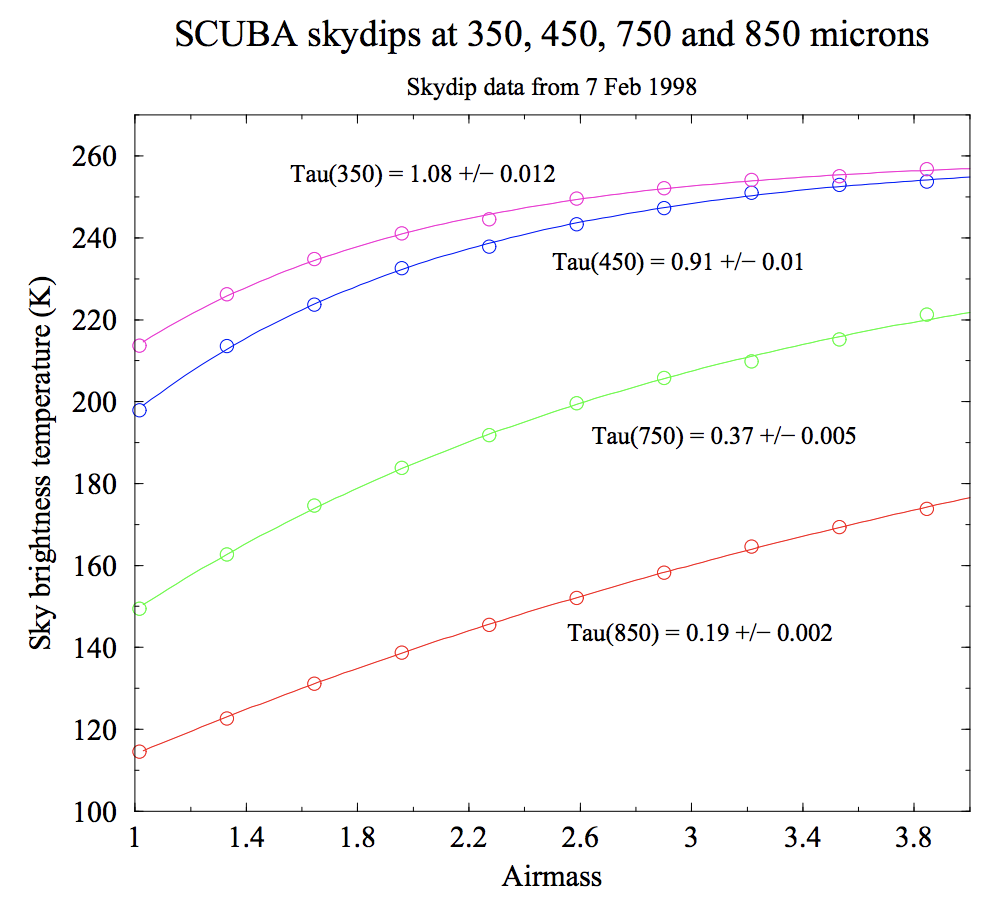
\includegraphics[width=0.5\textwidth]{tau.png}
   \end{center}
\caption[SCUBA Optical Loading Skydips -(\cite{Archibald2002})]{Optical Loading for Various Wavelengths to determine optical depth for the SCUBA instrument. The sky brightness is determined by performing telescope sky dips. The open circles here are the measurements taken at different airmasses (or elevations), and the solid line is the fit to the data which provides the optical depth. The conversion used by SCUBA is given in \cite{Archibald2002} by Equation 2. A similar model will be used by TIME, but with Rayleigh-Jeans temperature approximations. This type of graph will be produced by the Data Analysis Suite.}
\label{fig:tau}
\end{wrapfigure}
third cases are both run on archival data after calibration or observing tests have been completed. The data retrieval suite will have access to a series of directories that are named based on the Julian Date (JD) and type of data (either telescope or detector), and can be queried for other specifics including the observer, specific times, etc. The pre-processing pipeline will be available as a button on the interface that the user activates, and can include processes such as data decimation, removal of corrupted data, application of anti-aliasing filters, high pass filters, and atmospheric removal, to name a few. An example of this process in action is for determining the change in atmospheric loading on the detectors with elevation. The opacity of the atmosphere changes with elevation and effects the brightness of sources viewed through it. Fortunately, it can be characterized by sky dips, where the telescope is moved through various elevations, while the detectors record the sky brightness temperature. To accomplish the actual goal of measuring \(\tau \) , the raw data must be retrieved and then have several conversions to transform it from sky brightness to optical depth. This type of analysis requires a conversion from the voltage returned by the detector, to resistance, and then finally to the bolometer temperature. This temperature can be related back to the Rayleigh-Jeans equivalent temperature, and then used with a basic plane-parallel atmospheric model to determine \(\tau\) . These conversions will be automated, and present a plot of the subsequent analysis after the appropriate data is selected by the user. An example is shown in Figure ~\ref{fig:tau}.

\begin{center}
\begin{tabular}{|c|c|}
\hline
\textbf{Tests} & \textbf{Analysis}\\
\hline
\hline
  \tabitem Pointing Model & \tabitem Detector Noise\\
  \tabitem Beam Model & \tabitem Telescope Noise\\
  \tabitem Optical Loading for various El & \tabitem Raster Maps\\
  \tabitem Internal/Software Data Downsampling & \tabitem El Dips\\
  \tabitem Anti-Aliasing Method & \tabitem Sky Dips\\
  \tabitem Low/High Pass Filter & \tabitem Pointing Cross\\
  \tabitem Filter Deconvolution Technique & \tabitem Telescope Focus\\
  \tabitem Common Mode Atmospheric Template & \tabitem Detector Offsets\\
  \tabitem Load Curves (lab/telescope) & \tabitem Point Source Calibration\\
  \tabitem Atmospheric Conditions (airmass, water vapor, etc.) & \tabitem Beam Mapping/Fitting\\
\hline
\end{tabular}\label{table:pipeline}
\end{center}


\section{In Conclusion}

The TIME instrument will be integral to creating the first large sky survey of the kSZ effect, and improving upon measurements of CII and CO line intensities in galaxies and galaxy clusters. To accomplish this, it will be using a driven scan intensity mapping observing strategy, which has the advantages of quick integrations times, and a low spatial resolution, without the need to resolve individual galaxies. It will also be able to successfully remove atmospheric contamination from the data, and any other systematic noise, by taking multiple measurements of the same patch of sky across its 16 detectors. These improvements have the potential for many scientific insights, briefly summarized again below.

The kSZE will be mapped across multiple redshifts to a high significance, creating the first peculiar velocity maps of large scale structure. This map will be able to trace the gravitational potentials through cosmic time, without any dependence on the redshift being observed. From this we can generate theories about the role of dark matter production in the early universe and how it influenced the development of gravitational perturbations to the space-time metric. Dark matter is currently theorized to contribute 25\% of the matter energy density of the universe, which has been estimated from the anisotropies in the CMB and other methods. With this additional method of visualizing dark-baryonic matter interactions, these values can be corroborated through an independent technique. 

One additional use for observing kSZE is in determining the gas physics at work in the ICM. Since we are essentially measuring the motion, temperature, and possibly feedback and cooling outflows of the gas, a model for the hydrodynamical evolution of cluster gas with redshift can also be created. This is especially useful as a comparator to other cluster measurement techniques that rely heavily on the assumed gas clumping and density. More often these values are taken from local sources that may create some redshift correlated error when used outside the local cluster. This insight into gas dynamics is a shared trait with CII and CO measurements. While kSZE focuses mostly on the ICM, CII and CO can also reach the ISM and IGM (for isolated galaxies). In this case, the usefulness is in studying the transition of galaxies through the Epoch of Reionization and the Epoch of Peak Star Formation. CII can probe the ionized medium, while CO traces the neutral hydrogen reservoirs. The combination can reveal the ionization bubble size and development around primordial galaxies, the physics of the first ionizing sources, show the changing neutral gas reservoirs in galaxies, and allow modeling of changing stellar populations at different epochs. 

It is clear from the discussion above that TIME will have numerous contributions to the field of Cosmology, which is somewhat astounding considering it is all possible from a single experiment. Provided everything goes well, it should be making strides as early as the winter of 2018, with results from data analysis possibly a year after. The writer will be holding their breath in anticipation. 

%%%%%%%%%%%%%%%%%%%%%%%%%%%%%%%%%%%%%%%%%%%%%%%%%%%%%%%%%%%%%%%%%%%%%%%%%%%%%%%%%%
% REFERENCES
\newpage
\renewcommand\bibsection{\section{\refname}}
\bibliographystyle{unsrtnat}
\bibliography{references}

\newpage
\appendix


\end{document}
